\documentclass[utf8,usehyperref,12pt]{G7-32}
\usepackage{amsthm,amsfonts,amsmath,amssymb,amscd}
\usepackage[T2A]{fontenc}
\usepackage[utf8]{inputenc}
\usepackage[english,russian]{babel}
\usepackage{float}
\usepackage{graphicx}
\usepackage{cmap}
\usepackage{color}


\usepackage[all,cmtip]{xy}
\graphicspath{{pictures/}}

\usepackage{subcaption}
\usepackage{cite}

\usepackage{dsfont}
\usepackage{mathrsfs}
%\newtheorem{theoremA}{Теорема}
%\renewcommand*{\thetheoremA}{\Alph{theoremA}}

\TableInChaper
\PicInChaper
\setlength\GostItemGap{2mm}


\NirOrgLongName{\MakeUppercase{ФЕДЕРАЛЬНОЕ АГЕНТСТВО НАУЧНЫХ ОРГАНИЗАЦИЙ\\
ФЕДЕРАЛЬНОЕ ГОСУДАРСТВЕННОЕ БЮДЖЕТНОЕ УЧРЕЖДЕНИЕ НАУКИ \\ ДАГЕСТАНСКИЙ ФЕДЕРАЛЬНЫЙ ИССЛЕДОВАТЕЛЬСКИЙ ЦЕНТР РОССИЙСКОЙ АКАДЕМИИ НАУК}}

\NirBoss{Директор ДФИЦ РАН}{Муртазаев А.К.} %% Заказчик, утверждающий НИР
\NirManager{Врио зав. Отделом математики и информатики ИФ ДФИЦ РАН, кандидат физ.-мат. наук}{Шарапудинов Т.И.}

\NirTown{Махачкала,}
\NirYear{2023}

\NirUdk{УДК \No }
\NirGosNo{Регистрационный \No }

\NirStage{
}{промежуточный, за 2022 г.}{
}

\bibliographystyle{unsrt}

\newtheorem{theorem}{Теорема}[chapter]
\newtheorem*{theorem*}{Теорема}
\newtheorem*{lemma*}{Лемма}
\newtheorem*{abstract}{Аннотация}
\newtheorem{property}{Свойство}
\newtheorem{lemma}{Лемма}[chapter]
\newtheorem{statement}{Утверждение}[chapter]
\newtheorem{definition}{Определение}[chapter]
\newtheorem{example}{Пример}[chapter]
\newtheorem{corollary}{Следствие}[chapter]
\newtheorem*{corollary*}{Следствие}
\newtheorem{remark}{Замечание}[chapter]
\newtheorem*{remark*}{Замечание}
\newtheorem{hypothesis}{Гипотеза}[chapter]

\newtheorem{cond}{Условие}
\newtheorem{theoremA}{Теорема}[chapter]
\newtheorem{lemmaA}{Лемма}[chapter]
\newtheorem{corollaryA}{Следствие}[chapter]

\newtheorem{state}{Предложение}
\newtheorem{proposition}{Предложение}[chapter]
\renewcommand{\thetheoremA}{\thechapter.\Alph{theoremA}}
\renewcommand{\thelemmaA}{\thechapter.\Alph{lemmaA}}
\renewcommand{\thecorollaryA}{\thechapter.\Alph{corollaryA}}
\newcommand{\No}{\textnumero}

\newcommand{\norm}[1]{\|#1\|_{p(\cdot),w}}
\newcommand{\ip}[2]{\langle #1, #2 \rangle}

\DeclareMathOperator*{\esssup}{ess\,sup}
\DeclareMathOperator*{\essinf}{ess\,inf}

\numberwithin{equation}{chapter} %
\renewcommand{\theequation}{\thechapter.\arabic{equation}}

\newenvironment{description}{}{}

\DeclareMathOperator*{\sign}{sign}
\newtheorem{theoremrus}{Теорема}
\newtheorem{lemmarus}{Лемма}
\newtheorem{statementrus}{Утверждение}
\newtheorem{remarkrus}{Замечание}
\newtheorem{corollaryrus}{Следствие}



\def\Ker{\operatorname{Ker}}

\newcommand{\row}[3]{
  \small{#1}&
  \centering{\rule[-2mm]{5cm}{0.2mm}} \newline \centering \footnotesize{{подпись, дата}} &
  #2 \newline \small{{(#3)}} \\ & & \\
}

\usepackage[shortlabels]{enumitem}

%%%%%%%<------------- НАЧАЛО ДОКУМЕНТА
\begin{document}

% \usefont{T2A}{ftm}{m}{} %%% Использование шрифтов Т2 для возможности скопировать текст из PDF-файлов.

\frontmatter %%% <-- это выключает нумерацию ВСЕГО; здесь начинаются ненумерованные главы типа Исполнители, Обозначения и прочее

\NirTitle{\begin{center}
{\large
[НАЗВАНИЕ ТЕМЫ]
}
\\[12pt]
\end{center}
}

\Executors %% Список исполнителей здесь
% %%% это рисует линию размера 3мм и толщиной 0.1 пункт
\begin{longtable}{p{0.35\linewidth}p{0.2\linewidth}p{0.35\linewidth}}
\begin{longtable}{p{0.35\textwidth} p{0.3\textwidth} p{0.33\textwidth}}

    Руководитель НИР, вед. науч. \newline сотр. ОМИ, & & \\
    % \small{д-р физ.-мат. наук} &
    % \centering{\rule[-2mm]{5cm}{0.2mm}} \newline \centering \footnotesize{{подпись, дата}} &
    % Р.И. Кадиев \newline \small{{(раздел 6)}}  \\
    % & & \\
    \row{д-р физ.-мат. наук}{Р.И. Кадиев}{раздел 6}


    Отв. исполнители: & & \\

    \row{Гл. науч. сотр., д-р.ф.-м.н.}{А.-Р. К. Рамазанов}{раздел 3}
    \row{Вед. науч. сотр., д.ф.-м.н.}{А.М. Магомедов}{раздел 7}
    \row{Вед. науч. сотр., д.ф.-м.н.}{М.М. Сиражудинов}{раздел 7}
    \row{Зав. ОМИ, к.ф.-м.н.}{Т.И. Шарапудинов}{общ. ред.}


    Исполнители: & & \\
    
    \row{Ст. науч. сотр., к.ф.-м.н.}{М.Г. Магомед-Касумов}{раздел \ref{MMG}, введение}
    \row{Ст. науч. сотр., к.ф.-м.н.}{М.К. Рамазанов}{раздел 10}
    \row{Ст. науч. сотр., к.ф.-м.н.}{М.А. Магомедов}{раздел 9}
    \row{Ст. науч. сотр., к.ф.-м.н.}{З.Г. Меджидов}{раздел 8}
    \row{Науч. сотр.}{М.С. Султанахмедов}{введение, заключение}
    \row{Науч. сотр.}{Т.Н. Шах-Эмиров}{раздел 4}
    \row{Науч. сотр.}{Р.М. Гаджимирзаев}{раздел 2, реферат, введение}
    \row{Мл. науч. сотр.}{С.Р Магомедов}{раздел 6, заключение}
    \row{Мл. науч. сотр.}{Ш.М. Гаммадов}{разделы 8}
    \small{Нормоконтроль}&
    \centering{\rule[-2mm]{5cm}{0.2mm}} \newline \centering \footnotesize{{подпись, дата}} &
    М.С. Султанахмедов \\ & & \\

\end{longtable}

\end{longtable}

\Referat %Реферат отчёта, не более 1 страницы

Отчет X с., X рис., X таблиц, X источников.

\MakeUppercase{полиномы Якоби -- Соболева, полиномы Мейкснера -- Соболева, ряд Фурье, равномерная сходимость, пространства Соболева и Лебега, условия Макенхоупта, рациональные сплайны, уравнение Бельтрами, задача Римана -- Гильберта, W-метод, уравнение Ито, метод Ванга-Ландау.
}

Объектом исследования являются системы полиномов, ортогональные относительно дискретно-непрерывного скалярного произведения Соболева; интерполяционные рациональные сплайн-функции;
базисность полиномов Лежандра в пространствах Лебега с переменным показателем;
стохастические системы с запаздыванием;
усреднения периодической задачи для уравнения Бельтрами;
интегральные преобразования скалярных и векторных полей;
проверка интервальной раскрашиваемости всех биграфов заданного порядка;
чистые и разбавленные модели Поттса.

В ходе выполнения НИР изучена сходимость рядов Фурье по полиномам Якоби -- Соболева, Мейкснера -- Соболева и исследованы аппроксимативные свойства их частичных сумм в различных функциональных пространствах. Получены динамическое решение интегрального уравнения Вольтерры второго рода в виде коллокационных рациональных сплайн-функций и точные по порядку оценки скорости сходимости приближенных решений. Получено также приближенное решение интегрального уравнения Фредгольма второго рода в случае произвольных сеток узлов.
Получены утверждения, играющие важную роль при изучении базисности системы полиномов Лежандра в пространствах Лебега с переменным показателем.
Предложен и обоснован модифицированный метод регуляризации для анализа различных видов устойчивости стохастических систем, содержащий одновременно компоненты с непрерывным и дискретным временем, и получены достаточные условия моментной устойчивости решений для таких систем.
Изучены вопросы усреднения обобщенного уравнения Бельтрами с локально периодическими коэффициентами и получены оценки погрешности усреднения периодической задачи для обобщенного уравнения Бельтрами в пространствах Соболева и Лебега.
Получены новые формулы обращения интегральных преобразований скалярных и векторных полей, определенных на некоторых семействах ломаных на плоскости.
Разработано программное обеспечение для решения перечислительных проблем дискретной математики, задач компьютерной графики, а также для создания демонстрационного материала по дисциплинам компьютерных наук.
Методом Ванга-Ландау исследована трехвершинная модель Поттса на решетке Кагоме. 
Определены структуры основного состояния и построена фазовая диаграмма. 

Полученные результаты могут найти применение в задачах математической физики, цифровой обработки сигналов, теории управления и в задачах составления расписаний мультипроцессорной системы.


\setcounter{tocdepth}{2} %hide subsections

\tableofcontents

%\NormRefs % Нормативные ссылки
%\Defines % Необходимые определения

\Abbreviations %% Список обозначений и сокращений в тексте
В настоящем отчете о НИР применяют следующие сокращения и обозначения.
\begin{abbreviation}
\item[ДФИЦ] Дагестанский федеральный исследовательский центр
\item[ОМИ] Отдел математики и информатики
\item[РАН] Российская академия наук
\item[ФП] Фазовый переход
\item[ПО] Программное обеспечение
\end{abbreviation}

\Introduction

В последние годы теории ортогональных по Соболеву полиномов посвящено большое число работ. В частности, это связано с тем, что соболевские скалярные произведения и соответствующие им ортогональные системы (и их дифференциальные аналоги) играют важную роль во многих проблемах теории функций, квантовой механики, математической физики, вычислительной математики и т.д. В частности, ряды Фурье по ним обладают важными для приложений свойствами, которые отсутствуют у рядов Фурье по классическим ортогональным системам (см., например, \cite{Ram-Ba-Ra-Pe,Ram-Mar-Xu,Ram-Shar-UMN}).
Например, ряды Фурье по полиномам, ортогональным по Соболеву, представляется более естественным аппаратом, чем ряды Фурье по классическим ортогональным полиномам, для приближенного решения краевых задач, в которых требуется анализ поведения приближенного решения в одной или нескольких точках.
При решении таких задач важную роль играют сходимость и скорость сходимости рядов Фурье. В этом параграфе эти вопросы будут рассмотрены для систем полиномов, ортогональных по Соболeву и порожденных полиномами Якоби (см. п. \ref{Ram-Jac}) и Мейкснера (см. п. \ref{Ram-Mex}).



\mainmatter %% это включает нумерацию глав и секций в документе ниже

\section{Об аппроксимативных свойствах рядов Фурье по полиномам Якоби \texorpdfstring{\linebreak$P_n^{\alpha-r,-r}(x)$}{}, ортогональным по Соболеву}\label{Ram-Jac}
Пусть $-1<\alpha$ -- нецелое, $\rho(x)=(1-x)^\alpha$, $L_\rho^2$ -- пространство Лебега, состоящее из измеримых на $[-1,1]$ функций $f$, для которых
$$
\int_{-1}^{1}f^2(x)\rho(x)dx<\infty.
$$
Для $r\in\mathbb{N}$ через $W^r_{L_\rho^2}$ обозначим пространство функций $f$, непрерывно дифференцируемых $r-1$ раз, причем $f^{(r-1)}$ абсолютно непрерывна на $[-1,1]$, а $f^{(r)}\in L_\rho^2$, $W^r$ -- класс $r$ раз непрерывно дифференцируемых функций $f$, заданных на $[-1,1]$ и для которых $|f^{(r)}|\le 1$.
Для $f,g\in W^r_{L_\rho^2}$ определим скалярное произведение Соболева следующего вида
\begin{equation}\label{Ram-Sob_inner_product}
\langle f,g\rangle_S=\sum_{\nu=0}^{r-1}f^{(\nu)}(-1)g^{(\nu)}(-1)+\int_{-1}^{1}f^{(r)}(x)g^{(r)}(x)\rho(x)dx.
\end{equation}

Рассмотрим систему полиномов
\begin{equation}\label{Ram-Ort_Sob_pol}
	\varphi_n(x)=
	\begin{cases}
		\frac{(x+1)^n}{n!}, & 0\le n\le r-1 \\
		\frac{2^r}{(n+\alpha-r)^{[r]}\sqrt{h_{n-r}^{\alpha,0}}}P_n^{\alpha-r,-r}(x), & r\le n,
	\end{cases}
\end{equation}
где $P_n^{\alpha-r,-r}(x)$ -- полином Якоби степени $n$. В работе~\cite{Ram-SharMN} было показано, что система~\eqref{Ram-Ort_Sob_pol} полна в $W^r_{L_\rho^2}$ и ортонормирована относительно скалярного произведения~\eqref{Ram-Sob_inner_product}. Ряд Фурье по этой системе имеет следующий вид
\begin{equation}\label{Ram-Fourier_series} f(x)=\sum_{k=0}^{r-1}\frac{f^{(k)}(-1)}{k!}(x+1)^k+\sum_{k=r}^{\infty}\frac{2^r\widehat{f_k}P_k^{\alpha-r,-r}(x)}{\sqrt{h_{k-r}^{\alpha,0}}(k+\alpha-r)^{[r]}},
\end{equation}
где
$$
\widehat{f_k}=\langle f,\varphi_k\rangle_S=\int_{-1}^{1}f^{(r)}(t)\frac{P_{k-r}^{\alpha,0}(t)}{\sqrt{h_{k-r}^{\alpha,0}}}(1-t)^\alpha dt, \quad k\ge r.
$$

Через $S^\alpha_{n+2r}(f)=S^\alpha_{n+2r}(f,x)$ обозначим частичную сумму ряда~\eqref{Ram-Fourier_series}:
$$
S^\alpha_{n+2r}(f)=\sum_{k=0}^{r-1}\frac{f^{(k)}(-1)}{k!}(x+1)^k+
\sum_{k=r}^{n+2r}\frac{2^r\widehat{f_k}P_k^{\alpha-r,-r}(x)}{\sqrt{h_{k-r}^{\alpha,0}}(k+\alpha-r)^{[r]}}.
$$
В той же работе были исследованы аппроксимативные свойства сумм $S^\alpha_{n+2r}(f)$ для функций из пространства $W^r$. В частности была доказана следующая (см.~\cite[теорема 4]{Ram-SharMN})

\begin{theoremA}\label{GRM-th-A}
Пусть $-1<\alpha$ -- нецелое, $r\in\mathbb{N}$, $f\in W^r$. Тогда
\begin{multline}\label{Ram-ineq_f-S}
|f(x)-S^\alpha_{n+2r}(f)|\le c(r)\left(\frac{\sqrt{1-x^2}}{n+2r}\right)^r\omega\left(f^{(r)},\frac{\sqrt{1-x^2}}{n+2r}\right)+ \\
c(r)\left[\omega\left(f^{(r)},\frac{1}{n+2r}\right)\frac{I_{r,n}^\alpha(x)}{(n+2r)^r}+\omega\left(f^{(r)},\frac{1}{(n+2r)^2}\right)J_{r,n}^\alpha(x)\right],
\end{multline}
где
\begin{equation}\label{Ram-value_I}
I_{r,n}^\alpha(x)=(1+x)^r\int_{-1}^{1-1/n^2}(1-t)^{\alpha-\frac{r}{2}}(1+t)^{\frac{r}{2}}|K_{n+r}^{\alpha-r,r}(x,t)|dtб,
\end{equation}
\begin{equation}\label{Ram-value_J}
J_{r,n}^\alpha(x)=(1+x)^r\int_{1-1/n^2}^{1}(1-t)^{\alpha}|K_{n+r}^{\alpha-r,r}(x,t)|dt,
\end{equation}
$$
\omega(g,\delta)=\sup_{x,t\in[-1,1], |x-t|\le\delta}|f(x)-f(t)|.
$$
\end{theoremA}


В связи с неравенством~\eqref{Ram-ineq_f-S} возникает задача об оценке величин $I_{r,n}^\alpha(x)$ и $J_{r,n}^\alpha(x)$, определенных равенствами~\eqref{Ram-value_I} и~\eqref{Ram-value_J} соответственно. Основными результатами настоящего пункта являются теоремы~\ref{Ram-theo1} и~\ref{Ram-theo2}, в которых получены оценки сверху для $I_{r,n}^\alpha(x)$, $J_{r,n}^\alpha(x)$ при $x\in(-1,1)$.

В дальнейшем при оценке величин $I_{r,n}^\alpha(x)$, $J_{r,n}^\alpha(x)$ нам понадобятся некоторые преобразования формулы Кристоффеля -- Дарбу, определенной равенством~\eqref{Kris_Dar}. Для этого воспользуемся равенством~\eqref{alpha_1}, из которого находим
$$
P_{n+1}^{\alpha,\beta}(y)=\frac{n+\alpha+1}{n+1}P_{n}^{\alpha,\beta}(y)-\frac{2n+\alpha+\beta+2}{2(n+1)}(1-y)P_{n}^{\alpha+1,\beta}(y).
$$
С учетом этого равенства нетрудно получить оценку для ядра $K_n^{\alpha,\beta}(x,t)$:
$$
|K_n^{\alpha,\beta}(x,t)|\le
c(\alpha,\beta)\frac{n}{|x-t|}\left[(1-t)|P_{n}^{\alpha+1,\beta}(t)P_{n}^{\alpha,\beta}(x)|+
(1-x)|P_{n}^{\alpha+1,\beta}(x)P_{n}^{\alpha,\beta}(t)|\right].
$$
Если воспользоваться равенством~\eqref{beta_1}, то можно получить аналогичную оценку для \linebreak$K_n^{\alpha,\beta}(x,t)$:
$$
|K_n^{\alpha,\beta}(x,t)|\le
c(\alpha,\beta)\frac{n}{|x-t|}\left[(1+t)|P_{n}^{\alpha,\beta+1}(t)P_{n}^{\alpha,\beta}(x)|+
(1+x)|P_{n}^{\alpha,\beta+1}(x)P_{n}^{\alpha,\beta}(t)|\right].
$$

Теперь перейдем к формулировке основных результатов. Имеет место следующая
\begin{theorem}\label{Ram-theo1}
	Пусть $r-1<\alpha$ -- нецелое, $x\in(-1,1)$. Тогда для величины $I_{r,n}^\alpha(x)$ справедливы следующие оценки:
	
	1) если $x\in\left[0,1-\frac{1}{2n^2}\right]$, то
	\begin{equation*}
		I_{r,n}^\alpha(x)\le c(\alpha,r)(1-x)^{\frac{r}{2}}\left[\ln(n\sqrt{1-x}+1)+(1-x)^{-\frac{\alpha}{2}-\frac14}+1\right];
	\end{equation*}
	
	2) если $x\in\left(1-\frac{1}{2n^2},1\right)$, то
	\begin{equation*}
		I_{r,n}^\alpha(x)\le c(\alpha,r)
		\begin{cases}
			1, & \alpha\le r-\frac12, \\
			(1-x)^{\frac{r-\alpha}{2}-\frac14}, & \alpha>r-\frac12;
		\end{cases}
	\end{equation*}
	
	3) если $x\in\left[-1+\frac{1}{2n^2},0\right)$, то
	\begin{equation*}
		I_{r,n}^\alpha(x)\le c(\alpha,r)(1+x)^{\frac{r}{2}}\left(\ln(n\sqrt{1+x}+1)+(1+x)^{-\frac14}+1\right);
	\end{equation*}
	
	4) если $x\in\left(-1,-1+\frac{1}{2n^2}\right)$, то
	\begin{equation*}
		I_{r,n}^\alpha(x)\le c(\alpha,r)(1+x)^{\frac{r}{2}-\frac14}.
	\end{equation*}
\end{theorem}

Перейдем теперь к оценке величины $J_{r,n}^\alpha(x)$, определенной равенством~\eqref{Ram-value_J}. Справедлива следующая

\begin{theorem}\label{Ram-theo2}
	Пусть $r-1<\alpha$ -- нецелое, $x\in(-1,1)$. Тогда для величины $J_{r,n}^\alpha(x)$ справедливы следующие оценки:
	
	1) если $x\in\left(1-\frac{2}{n^2},1\right)$, то
	\begin{equation*}\label{est_for_J1_seg}
		J_{r,n}^\alpha(x)\le \frac{c(\alpha,r)}{n^{2r}},
	\end{equation*}
	
	2) если $x\in\left[0,1-\frac{2}{n^2}\right]$, то
	\begin{equation*}
		J_{r,n}^\alpha(x)\le c(\alpha,r)\frac{(1-x)^{\frac{r-\alpha}{2}-\frac34}}{n^{r+\alpha+\frac32}},
	\end{equation*}
	
	3) если $x\in(-1,0)$, то
	\begin{equation*}
		J_{r,n}^\alpha(x)\le c(\alpha,r)\frac{(1+x)^{\frac{r}{2}-\frac14}}{n^{r+\alpha+\frac32}}.
	\end{equation*}
\end{theorem}

Таким образом, сравнивая оценки для величин $I_{r,n}^\alpha(x)$ и $J_{r,n}^\alpha(x)$, мы можем переформулировать теорему \ref{GRM-th-A} в следующем виде.
\begin{theorem}\label{Ram-theo3}
Пусть $r\in\mathbb{N}$, $r-1<\alpha$ -- нецелое, $f\in W^r$, $x\in(-1,1)$. Тогда
\begin{equation*}
|f(x)-S^\alpha_{n+2r}(f)|\le \frac{c(\alpha,r)}{(n+2r)^r}\omega\left(f^{(r)},\frac{1}{n+2r}\right)\mathcal{I}_{r,n}^\alpha(x),
\end{equation*}
где
$$
\mathcal{I}_{r,n}^\alpha(x)=
\begin{cases}
     (1-x)^{\frac{r}{2}}\left[\ln(n\sqrt{1-x}+1)+(1-x)^{-\frac{\alpha}{2}-\frac14}+1\right], & 0\le x\le 1-\frac{1}{2n^2}; \\
     \begin{cases}
	       1, & \alpha\le r-\frac12, \\
	       (1-x)^{\frac{r-\alpha}{2}-\frac14}, & \alpha>r-\frac12,
     \end{cases} & 1-\frac{1}{2n^2}<x<1;\\
    (1+x)^{\frac{r}{2}}\left(\ln(n\sqrt{1+x}+1)+(1+x)^{-\frac14}+1\right), & -1+\frac{1}{2n^2}\le x<0; \\
    (1+x)^{\frac{r}{2}-\frac14}, & -1<x<-1+\frac{1}{2n^2}.
\end{cases}
$$
\end{theorem}


\chapter{Ряды Фурье по полиномам Мейкснера -- Соболева}\label{Ram-Mex}
\section{Введение}
В литературе можно встретить различные подходы к построению систем полиномов, ортогональных по Соболеву, отличающиеся выбором тех или иных скалярных произведений.
Приведем некоторые виды скалярных произведений, связанные с полиномами Мейкснера.
Например, в \cite{Ram-Ar-Go-Mar,Ram-Kh-Old} рассмотрено скалярное произведение Соболева следующего вида
$$
\langle f,g\rangle_S=\sum_{x=0}^{\infty}f(x)g(x)w(x)+\lambda\sum_{x=0}^{\infty}\Delta f(x)\Delta g(x)w(x),
$$
где $\lambda\ge 0$, $\Delta f(x)=f(x+1)-f(x)$, $w(x)$ -- вес Мейкснера. А в \cite{Ram-Bav1,Ram-Bav2} были рассмотрены частные случаи этого скалярного произведения, а именно, в \cite{Ram-Bav1} вместо второй суммы было рассмотрено одно слагаемое $\lambda f(0)g(0)$, в \cite{Ram-Bav2} -- два слагаемых $Mf(0)g(0)+N\Delta f(0)\Delta g(0)$, $M,N\ge 0$. При этом было показано, что полиномы $\{Q_n(x)\}$, ортогональные относительно этих скалярных произведений, можно определить посредством равенства $Q_n(x)=\sum_{k=0}^{n}c_{k,n}M_k^\alpha(x)$, где $M_k^\alpha(x)$ -- полином Мейкснера степени $k$. Далее, в \cite{Ram-Shar-VMJ,Ram-Shar-Sar} было рассмотрено скалярное произведение следующего вида
\begin{equation}\label{Ram-Sob-inner-Intro}
\langle f,g\rangle_S=\sum_{k=0}^{r-1}\Delta^kf(0)\Delta_\delta^kg(0)+\sum_{x=0}^\infty\Delta^rf(x)\Delta^rg(x)w(x)
\end{equation}
и показано, что полиномы, ортонормированные относительно \eqref{Ram-Sob-inner-Intro}, можно определить посредством равенств
$$
m_{r,n}^{\alpha}(x)=\frac{x^{[n]}}{n!},\ n=\overline{0,r-1},
$$
$$
m_{r,n}^{\alpha}(x)=
\frac{1}{\sqrt{h_{n-r}^\alpha}(r-1)!}\sum_{t=0}^{x-r}(x-1-t)^{[r-1]}M_{n-r}^\alpha(t),\ x\ge r,\ n\ge r,
$$
где $x^{[n]}=x(x-1)\cdots(x-n+1)$.
В дальнейшем нам понадобятся некоторые обозначения. Пусть $1\le p<\infty$, $l_w^p(\Omega)$ -- пространство дискретных функций $f$, заданных на сетке $\Omega=\{0, 1, \ldots\}$ и для которых $\|f\|_{l_{w}^p(\Omega)}^p=\sum_{x\in\Omega}|f(x)|^pw(x)<\infty$, а $W^r_{l_{w}^p(\Omega)}$ -- подпространство в $l_{w}^p(\Omega)$.
В \cite{Ram-Shar-Sar} была доказана следующая

\begin{theoremA}\label{GRM-th-B}
Система полиномов $\{m_{r,n}^\alpha(x)\}$ полна в $W^r_{l_w^2(\Omega)}$.
\end{theoremA}

Другие виды скалярных произведений Соболева, связанные с полиномами Мейкснера, можно найти в \cite{Ram-Mor-Bal,Ram-Co-So-Vil}.
Результаты, полученные в вышеприведенных работах \cite{Ram-Shar-VMJ,Ram-Ar-Go-Mar,Ram-Kh-Old,Ram-Bav1,Ram-Bav2,Ram-Shar-Sar,Ram-Mor-Bal,Ram-Co-So-Vil}, в основном связаны с исследованием распределения нулей полиномов Мейкснера --  Соболева, изучением их алгебраических, асимптотических и дифференциальных свойств. В то же время остаются мало изученными вопросы сходимости ряда Фурье по полиномам Мейкснера -- Соболева и аппроксимативные свойства его частичных сумм. В связи с этим в отчетном году была рассмотрена система полиномов $\{m_{n,N}^{\alpha,r}(x)\}$, ортонормированная по Соболеву и порожденная системой модифицированных полиномов Мейкснера $\{m_{n,N}^{\alpha}(x)\}$.
Показано, что ряд Фурье по этой системе сходится к $f\in W^r_{l^p_{\rho_N}(\Omega_\delta)}$ поточечно на сетке $\Omega_\delta$ при $p\ge2$. А в случае, когда $1\le p<2$ показано, что существуют функция и сетка $\Omega_\delta$, ряд Фурье которой расходится в некоторой точке $x_0\in\Omega_\delta$. Кроме того, исследованы аппроксимативные свойства частичных сумм ряда Фурье по системе $\{m_{n,N}^{0,r}(x)\}$.

\section{Некоторые сведения о полиномах Мейкснера}

Пусть $N>0$, $\delta=1/N$, $\Omega_\delta=\{0,\delta,2\delta,\ldots \}$. Через $M_{n,N}^{\alpha}(x)$ обозначим модифицированные полиномы Мейкснера, которые при $\alpha>-1$ ортогональны на сетке $\Omega_\delta$ относительно веса $\rho_N(x)=e^{-x}\frac{\Gamma(Nx+\alpha+1)}{\Gamma(Nx+1)}(1-e^{-\delta})^{\alpha+1}$. Соответствующие ортонормированные полиномы мы обозначим через $m_{n,N}^{\alpha}(x)=\frac{1}{\sqrt{h_n^\alpha}}M_{n,N}^{\alpha}(x)$, где $h_n^\alpha={\binom{n+\alpha}{n}}e^{n\delta}\Gamma(\alpha+1)$. Приведем некоторые свойства полиномов $M_{n,N}^{\alpha}(x)$, которые можно найти в \cite{Ram-SharBook}:
\begin{itemize}
\item
формула Родрига
\begin{equation}\label{Ram-for-Rod}
M_{n,N}^{\alpha}(x)=\frac{\Gamma(Nx+1)e^{n\delta+x}}{n!\Gamma(Nx+\alpha+1)}
\Delta^n_\delta\left\{\frac{\Gamma(Nx+\alpha+1)}
{\Gamma(Nx-n+1)}e^{-x}\right\};
\end{equation}
\item
явный вид
\begin{equation}\label{Ram-explicit-rep}
M_{n,N}^\alpha(x)={\binom{n+\alpha}{n}}\sum_{k=0}^n{\frac{n^{[k]}(Nx)^{[k]}}{(\alpha+1)_kk!}}\left(1-e^\delta\right)^k;
\end{equation}
\item
равенства
\begin{equation}\label{Ram-deriv}
\Delta_\delta^r M_{n,N}^{\alpha}(x)=(1-e^{\delta})^rM_{n-r,N}^{\alpha+r}(x),
\end{equation}
\begin{equation}\label{Ram-parametr-r}
M^{-l}_{n,N}(x)=\frac{(n-l)!}{n!}(e^\delta-1)^l(-Nx)_lM_{n-l,N}^l(x-l\delta),\ 1\le l\le n;
\end{equation}

\item
формула Кристоффеля--Дарбу
\begin{multline}\label{Ram-Kric-Dar}
K_{n,N}^{\alpha}(x,y)=\sum_{k=0}^n m_{k,N}^{\alpha}(x)m_{k,N}^{\alpha}(y)=\\
\frac{\delta}{(e^{\delta}-1)e^{n\delta}}\frac{(n+1)!}{\Gamma(n+\alpha+1)}\frac{M_{n,N}^\alpha(x)M_{n+1,N}^\alpha(y)-
M_{n+1,N}^\alpha(x)M_{n,N}^\alpha(y)}{x-y},
\end{multline}
\end{itemize}
которую посредством элементарных преобразований можно записать в следующем виде
$$
K_{n,N}^\alpha(x,y)={\frac{\alpha_n}{(\alpha_n+\alpha_{n-1})}}m_{n,N}^{\alpha}(x)m_{n,N}^{\alpha}(y)+
{\frac{\alpha_n\alpha_{n-1}}{\alpha_n+\alpha_{n-1}}}{\frac{\delta}{e^{\frac{\delta}{2}}-e^{-{\frac{\delta}{2}}}}} {\frac{1}{y-x}}\times
$$
$$
\left[m_{n,N}^\alpha(y)\left(m_{n+1,N}^\alpha(x)- m_{n-1,N}^\alpha(x)\right)
-m_{n,N}^\alpha(x)\left(m_{n+1,N}^\alpha(y)-m_{n-1,N}^\alpha(y)
\right)\right],
$$
где $\alpha_n=\sqrt{(n+1)(n+\alpha+1)}$.

Далее, при $\alpha>-1$, $0\le x<\infty$, $\theta_n=4n+2\alpha+2$, $\lambda>0$, $1\le n\le \lambda N$, $s\geq0$ справедливы следующие весовые оценки~\cite{Ram-SharBook}:
\begin{equation*}
e^{-x/2}\left|m_{n,N}^\alpha(x\pm s\delta)\right|\le c(\alpha,\lambda,s)\theta_n^{-\frac{\alpha}{2}}A_n^\alpha(x),
\end{equation*}
\begin{equation*}
A_n^\alpha(x)=\begin{cases}
\theta_n^{\alpha},&  0\le x\le \frac{1}{\theta_n},\\
\theta_n^{\alpha/2-1/4}x^{-\alpha/2-1/4},&     \frac{1}{\theta_n}<x\le {\frac{\theta_n}{2}},\\
\left[\theta_n(\theta_n^{1/3}+|x-\theta_n|)\right]^{-1/4},& {\frac{\theta_n}{2}}<x\leq{\frac{3\theta_n}{2}},\\
e^{-x/4}, & {\frac{3\theta_n}{2}}<x<\infty,
\end{cases}
\end{equation*}
$$
e^{-x/2}\left|m_{n+1,N}^{\alpha}(x)-m_{n-1,N}^{\alpha}(x)\right|\leq
$$
\begin{equation*}
c(\alpha,\lambda)\begin{cases}
\theta_n^{\alpha/2-1},&  0\le x\le \frac{1}{\theta_n},\\
\theta_n^{-3/4}x^{-\alpha/2+1/4},&     \frac{1}{\theta_n}<x\le {\frac{\theta_n}{2}},\\
x^{-\alpha/2}\theta_n^{-3/4}\left[\theta_n^{1/3}+|x-\theta_n|\right]^{1/4},& {\frac{\theta_n}{2}}<x\leq{\frac{3\theta_n}{2}},\\
e^{-x/4}, & {\frac{3\theta_n}{2}}<x<\infty,
\end{cases}
\end{equation*}
где здесь и далее $c(\alpha)$, $c(\alpha, \lambda)$, $c(\alpha, \lambda, s)$ -- положительные числа, зависящие только от указанных параметров, причем различные в разных местах.

В дальнейшем нам также понадобятся следующие утверждения.
\begin{lemma}
Пусть $0\le l$ -- целое, $r\in\mathbb{N}$, $l\le r$. Тогда имеет место равенство:
\begin{equation*}
\Delta^l_\delta\left((Nx)^{[r]}M^r_{n,N}(x-r\delta)\right)=(n-l+r+1)_l(Nx)^{[r-l]}M^{r-l}_{n,N}(x-(r-l)\delta).
\end{equation*}
\end{lemma}

\begin{lemma}[\cite{Ram-MN2019}]
Пусть $-1<\alpha\in\mathbb{R}$, $\theta_n=4n+2\alpha+2$, $\lambda>0$, $N=1/\delta$, $0<\delta\leq1$. Тогда для $1\leq n\leq \lambda N$ имеет место следующая оценка
\begin{equation*}
e^{-x}K_{n,N}^\alpha(x,x)\le c(\alpha,\lambda)
\begin{cases}
n^{1-\alpha}(A_n^\alpha(x))^2, & x\in[0,\frac{\theta_n}{2}]\cup[\frac{3\theta_n}{2},\infty), \\
n^{-\alpha}, & x\in[\frac{\theta_n}{2},\frac{3\theta_n}{2}].
\end{cases}
\end{equation*}
\end{lemma}

\section{Ряд Фурье и аппроксимативные свойства его частичных сумм}

Пусть $\alpha>-1$. Рассмотрим систему полиномов $\{m_{n,N}^{\alpha,r}(x)\}$:
\begin{equation*}
m_{n,N}^{\alpha,r}(x)=\frac{(Nx)^{[n]}}{n!},\ n=\overline{0,r-1},
\end{equation*}
\begin{equation}\label{Ram-Pol-second}
m_{n,N}^{\alpha,r}(x)=
\frac{1}{(r-1)!}\sum\limits_{t\in \Omega_\delta^x}(Nx-1-Nt)^{[r-1]}m_{n-r,N}^\alpha(t),\ x\ge r\delta,\ n\ge r.
\end{equation}
где $x^{[n]}=x(x-1)\cdots(x-n+1)$, $\Omega_\delta^x=\{0, \delta, \ldots, x-r\delta\}$. Заметим, что $m_{n,N}^{\alpha,r}(x)=0$ при $n\ge r$, $x\in\{0, \delta, \ldots, (r-1)\delta\}$. Действительно, из~\eqref{Ram-Pol-second} и~\eqref{Ram-explicit-rep} имеем
$$
m_{n,N}^{\alpha,r}(x)=\frac{1}{\sqrt{h_{n-r}^\alpha}}
{\binom{n-r+\alpha}{n-r}}\sum_{k=0}^{n-r}{\frac{(n-r)^{[k]}\left(1-e^\delta\right)^k}{(\alpha+1)_kk!}}P_{k+r}(x),
$$
где $P_{k+r}(x)=\frac{1}{(r-1)!}\sum\limits_{t\in \Omega_\delta^x}(Nx-1-Nt)^{[r-1]}(Nx)^{[k]}$. Запишем дискретный аналог формулы Тейлора для функции $d(x)=(Nx)^{[k+r]}$:
$$
d(x)=\sum_{k=0}^{r-1}\Delta_\delta^kd(0)\frac{(Nx)^{[k]}}{k!}+\frac{1}{(r-1)!}\sum\limits_{t\in \Omega_\delta^x}(Nx-1-Nt)^{[r-1]}\Delta^r_\delta d(x)=
$$
$$
\sum_{k=0}^{r-1}\Delta_\delta^kd(0)\frac{(Nx)^{[k]}}{k!}+(k+r)^{[r]}P_{k+r}(x)=(k+r)^{[r]}P_{k+r}(x).
$$
Отсюда $P_{k+r}(x)=\frac{d(x)}{(k+r)^{[r]}}=\frac{(Nx)^{[k+r]}}{(k+r)^{[r]}}$. А поскольку $(Nx)^{[k+r]}=0$ для $k\ge0$, $x\in\{0, \delta, \ldots, (r-1)\delta\}$, то $m_{n,N}^{\alpha,r}(x)=0$ при $n\ge r$, $x\in\{0, \delta, \ldots, (r-1)\delta\}$.

Если теперь запишем дискретный аналог формулы Тейлора для полинома $M_{n,N}^{\alpha-r}(x)$ и воспользуемся равенством~\eqref{Ram-deriv}, то получим
$$
M_{n,N}^{\alpha-r}(x)=\sum_{k=0}^{r-1}\Delta_\delta^kM_{n,N}^{\alpha-r}(0)\frac{(Nx)^{[k]}}{k!}+
\frac{(1-e^\delta)^r}{(r-1)!}\sum\limits_{t\in \Omega_\delta^x}(Nx-1-Nt)^{[r-1]}M_{n-r,N}^{\alpha}(x).
$$
Отсюда с учетом~\eqref{Ram-Pol-second} имеем
\begin{equation}\label{Ram-rep-alpha-r}
m_{n,N}^{\alpha,r}(x)= \frac{1}{(1-e^\delta)^r}\frac{1}{\sqrt{h_{n}^{\alpha}}}\left[M_{n,N}^{\alpha-r}(x)-\sum_{k=0}^{r-1}\Delta_\delta^kM_{n,N}^{\alpha-r}(0)\frac{(Nx)^{[k]}}{k!}\right],
\end{equation}
где $\Delta^k_\delta M_{n,N}^{\alpha-r}(0)=(1-e^\delta)^k\frac{\Gamma(n+\alpha-r+1)}{(n-k)!\Gamma(\alpha-r+k+1)}$. Заметим, что $\Delta^k_\delta M_{n,N}^{\alpha-r}(0)=0$ при $\alpha=0$.

Из определения системы $\{m_{n,N}^{\alpha,r}(x)\}$ также вытекает следующее свойство:
\begin{equation}\label{Ram-deriv-for-sys}
\Delta_\delta^\nu m_{n,N}^{\alpha,r}(x)=
\begin{cases}
m_{n-\nu,N}^{\alpha,r-\nu}(x),& 0\le\nu\le r-1, r\le n,\\
m_{n-r,N}^{\alpha}(x),& \nu=r\le n,\\
m_{n-\nu,N}^{\alpha,r-\nu}(x),& \nu\le n<r,\\
0,& n<\nu\le r.
\end{cases}
\end{equation}
Из~\eqref{Ram-deriv-for-sys} следует, что система $\{m_{n,N}^{\alpha,r}(x)\}$ ортонормирована относительно скалярного произведения следующего вида
\begin{equation*}
\langle f,g\rangle_S=\sum_{k=0}^{r-1}\Delta_\delta^kf(0)\Delta_\delta^kg(0)+\sum_{x\in\Omega_\delta}\Delta_\delta^rf(x)\Delta_\delta^rg(x)\rho_N(x).
\end{equation*}

Из теоремы \ref{GRM-th-B} следует, что система полиномов $\{m_{n,N}^{\alpha,r}(x)\}$ полна в пространстве $W^r_{l^2_{\rho_N}(\Omega_\delta)}$. Нетрудно проверить, что ряд Фурье функции $f\in W^r_{l^2_{\rho_N}(\Omega_\delta)}$ по этой системе имеет следующий вид
\begin{equation}\label{Ram-Fourier-series}
f(x)\sim \sum_{k=0}^{r-1}\Delta_\delta^kf(0){\frac(Nx)^{[k]}{k!}}+\sum_{k=r}^\infty c^\alpha_{r,k}(f)m^{\alpha,r}_{k,N}(x),
\end{equation}
где
\begin{equation*}
c^\alpha_{r,k}(f)=\sum_{t\in\Omega_\delta}\Delta_\delta^r f(t)m^\alpha_{k-r,N}(t)\rho_N(t),\ k\ge r.
\end{equation*}
Из неравенства Гельдера следует, что коэффициенты $c^\alpha_{r,k}(f)$ существуют для любой функции $f\in W^r_{l^p_{\rho_N}(\Omega_\delta)}$ при $p\ge 1$. В связи с этим возникает вопрос о сходимости ряда Фурье~\eqref{Ram-Fourier-series} к функции $f\in W^r_{l^p_{\rho_N}(\Omega_\delta)}$. Справедлива следующая
\begin{theorem}\label{Ram-theoMex1}
Пусть $\alpha>-1$, $1\le p<\infty$. Тогда, если $f\in W^r_{l^p_{\rho_N}(\Omega_\delta)}$, то при $p\ge2$ ряд~\eqref{Ram-Fourier-series} сходится поточечно к $f$ на $\Omega_\delta$. Если же $1\le p<2$, то существуют сетка $\Omega_\delta$ и функция $f\in W^r_{l^p_{\rho_N}(\Omega_\delta)}$, ряд Фурье которой расходится в некоторой точке $x_0\in \Omega_\delta$.
\end{theorem}

Далее, через $S_{n+r,N}^{\alpha,r}(f,x)$ обозначим частичную сумму ряда~\eqref{Ram-Fourier-series}:
\begin{equation}\label{Ram-Part-sum}
S_{n+r,N}^{\alpha,r}(f,x)=\sum_{k=0}^{r-1}\Delta_\delta^kf(0)\frac{(Nx)^{[k]}}{k!}+\sum_{k=r}^{n+r} c^\alpha_{r,k}(f)m^{\alpha,r}_{k,N}(x).
\end{equation}
Из~\eqref{Ram-Part-sum} следует, что для $S_{n+r,N}^{\alpha,r}(x)$ имеют место равенства
\begin{equation*}
S_{n+r,N}^{\alpha,r}(f,x)=f(x), \quad x\in\{0, \delta, \ldots, (r-1)\delta\}.
\end{equation*}
Кроме того, если $f(x)=p_{n+r}(x)$ -- алгебраический полином степени не выше $n+r$, то
\begin{equation*}
S_{n+r,N}^{\alpha,r}(p_{n+r},x)\equiv p_{n+r}(x).
\end{equation*}

Рассмотрим теперь вопрос об аппроксимативных свойствах частичных сумм \\$S_{n+r,N}^{\alpha,r}(f,x)$ при $\alpha=0$. В этом случае из~\eqref{Ram-rep-alpha-r} и~\eqref{Ram-parametr-r} следует, что для $m_{n+r,N}^{0,r}(x)$ имеет место равенство
$$
m_{n+r,N}^{0,r}(x)=\frac{(Nx)^{[r]}}{\sqrt{(n+r)^{[r]}}}m_{n,N}^r(x-r\delta).
$$
Тогда~\eqref{Ram-Part-sum} можно записать в виде
\begin{equation*}
S_{n+r,N}^{0,r}(f,x)=\sum_{k=0}^{r-1}\Delta_\delta^kf(0){\frac{(Nx)^{[k]}}{k!}}+(Nx)^{[r]}\sum_{k=r}^{n+r} c^0_{r,k}(f)\frac{m^{r}_{k-r,N}(x-r\delta)}{\sqrt{k^{[r]}}}.
\end{equation*}

Далее, через $q_{n+r}(x)$ алгебраический полином степени $n+r,$ для которого
$
\Delta^i_\delta f(0)=\Delta^i_\delta q_{n+r}(0)\ (i=\overline{0, r-1}).
$
Тогда
$$
\left|f(x)-S_{n+r,N}^{0,r}(f,x)\right|\leq\left|f(x)-q_{n+r}(x)\right|+\left|S_{n+r,N}^{0,r}(q_{n+r}-f,x)\right|.
$$
Отсюда для $x\in\Omega_{r,\delta}=\{r\delta, (r+1)\delta, \ldots\}$
$$
e^{-{\frac{x}{2}}}x^{-{\frac{r}{2}}+{\frac{1}{4}}}\left|f(x)-S_{n+r,N}^{0,r}(f,x)\right|\leq e^{-{\frac{x}{2}}}x^{-{\frac{r}{2}}+{\frac{1}{4}}}\left|f(x)-q_{n+r}(x)\right|+
$$
\begin{equation}\label{Ram-gadz-eq15}
e^{-{\frac{x}{2}}}x^{-{\frac{r}{2}}+{\frac{1}{4}}}\left|S_{n+r,N}^{0,r}(q_{n+r}-f,x)\right|.
\end{equation}
Так как $\sum\limits_{k=0}^{r-1}\Delta_\delta^k(q_{n+r}(0)-f(0))\frac{(Nx)^{[k]}}{k!}=0$, то
$$
S_{n+r,N}^{0,r}(q_{n+r}-f,x)=
(Nx)^{[r]}\sum_{k=r}^{n+r}c_{r,k}^0(q_{n+r}-f) \frac{m^{r}_{k-r,N}(x-r\delta)}{\sqrt{k^{[r]}}}=
$$
$$
(Nx)^{[r]}\sum_{k=r}^{n+r}\frac{m^{r}_{k-r,N}(x-r\delta)}{\sqrt{k^{[r]}}}
\sum_{t\in\Omega_{\delta}}\Delta_\delta^r(q_{n+r}(t)-f(t))e^{-t}(1-e^{-\delta})m_{k-r,N}^0(t).
$$
К внутренней сумме применим преобразование Абеля (попутно воспользуемся равенствами \eqref{Ram-for-Rod}, \eqref{Ram-parametr-r}) и получим
$$
\sum_{t\in\Omega_{\delta}}\Delta_\delta^r(q_{n+r}(t)-f(t))e^{-t}(1-e^{-\delta})m_{k-r,N}^0(t)=
$$
$$
(-1)^r(1-e^{-\delta})\sum_{t\in\Omega_{\delta}}(q_{n+r}(t+r\delta)-f(t+r\delta))\frac{\sqrt{e^{(k-r)\delta}}}{(k-r)!}
\Delta_\delta^k\left\{\frac{\Gamma(Nt+1)e^{-t}}{\Gamma(Nt-k+r+1)}\right\}=
$$
$$
(-1)^r\frac{1-e^{-\delta}}{\sqrt{e^{(k-r)\delta}}}\sum_{t\in\Omega_{r,\delta}}(q_{n+r}(t)-f(t))\frac{\Gamma(Nt-r+1)}{\Gamma(Nt+1)}e^{-t}M_{k,N}^{-r}(t)=
$$
$$
\frac{(e^{\delta}-1)^{r+1}}{e^\delta}\sum_{t\in\Omega_{r,\delta}}(q_{n+r}(t)-f(t))e^{-t}\sqrt{k^{[r]}}m_{k-r,N}^{r}(t-r\delta).
$$
Тогда
$$
S_{n+r,N}^{0,r}(q_{n+r}-f,x)=\frac{(e^{\delta}-1)^{r+1}}{e^\delta}(Nx)^{[r]}\sum_{t\in\Omega_{r,\delta}}(q_{n+r}(t)-f(t))e^{-t}K_{n,N}^r(t-r\delta,x-r\delta).
$$
Отсюда и из \eqref{Ram-gadz-eq15} выводим
\begin{multline}\label{Ram-gadz-eq16}
e^{-{\frac{x}{2}}}x^{-{\frac{r}{2}}+{\frac{1}{4}}}\left|f(x)-S_{n+r,N}^{0,r}(f,x)\right|\leq e^{-{\frac{x}{2}}}x^{-{\frac{r}{2}}+{\frac{1}{4}}}\left|f(x)-q_{n+r}(x)\right|+\\
\frac{(e^{\delta}-1)^{r+1}}{e^\delta}e^{-{\frac{x}{2}}}x^{-{\frac{r}{2}}+{\frac{1}{4}}}(Nx)^{[r]}\sum_{t\in\Omega_{r,\delta}}(q_{n+r}(t)-f(t))e^{-t}K_{n,N}^r(t-r\delta,x-r\delta).
\end{multline}

Положим
\begin{equation}\label{Ram-gadz-eq17}
E_{k}^r(f,\delta)=\inf_{q_{k}}\sup_{x\in\Omega_{r,\delta}} e^{-{\frac{x}{2}}}x^{-{\frac{r}{2}}+{\frac{1}{4}}}\left|f(x)-q_{k}(x)\right|,
\end{equation}
где нижняя грань берется по всем алгебраическим полиномам $q_{k}(x)$ степени $k,$ для которых $\Delta_\delta^i f(0)=\Delta_\delta^i q_{k}(0)\ (i=\overline{0, r-1}).$
Тогда из \eqref{Ram-gadz-eq16} и \eqref{Ram-gadz-eq17} получаем
\begin{equation}\label{Ram-LebIne}
e^{-{\frac{x}{2}}}x^{-{\frac{r}{2}}+{\frac{1}{4}}}\left|f(x)-S_{n+r,N}^{0,r}(f,x)\right|\leq E_{n+r}^r(f,\delta)(1+\lambda_{n,N}^{r}(x)),
\end{equation}
где
$$
\lambda_{n,N}^{r}(x)=\frac{(e^{\delta}-1)^{r+1}}{e^\delta}e^{-{\frac{x}{2}}}x^{-{\frac{r}{2}}+{\frac{1}{4}}}(Nx)^{[r]}
\sum_{t\in\Omega_{r,\delta}}e^{-{\frac{t}{2}}}t^{{\frac{r}{2}}-{\frac{1}{4}}}
\left|K_{n,N}^r(t-r\delta,x-r\delta)\right|.
$$
В связи с неравенством \eqref{Ram-LebIne} возникает задача об оценке величины $\lambda_{n,N}^{r}(x)$ на $[r\delta,\infty)$. Пусть $\nu=4n+2r+2$. Введем обозначения:
$X_1=\left[r\delta, \frac{3}{\nu}\right]$,
$X_2=\left(\frac{3}{\nu}, \frac{\nu}{2}\right]$,
$X_3=\left(\frac{\nu}{2}, \frac{3\nu}{2}\right]$,
$X_4=\left(\frac{3\nu}{2}, \infty\right)$.
Справедлива следующая
\begin{theorem}\label{Ram-theoMex2}
Пусть $r\in\mathbb{N}$, $\lambda> 0$, $n\leq\lambda N.$ Тогда имеют место следующие оценки:\\
1) если $x\in X_1\cup X_2$, то
$$
\lambda_{n,N}^{r}(x)\leq c(\lambda, r)\ln (n+1);
$$
2) если $x\in X_3$, то
$$
\lambda_{n,N}^{r}(x)\leq c(\lambda,r)\left[\ln(n+1)+\left(\frac{\nu}{\nu^{\frac{1}{3}}+|x-\nu|}\right)^{\frac{1}{4}}\right];
$$
3) если $x\in X_4$, то
$$
\lambda_{n,N}^{r}(x)\leq c(\lambda,r)n^{-{\frac{r}{2}}+{\frac{7}{4}}}x^{{\frac{r}{2}}+{\frac{1}{4}}}e^{-\frac{x}{4}}.
$$
\end{theorem}





	





 \chapter{Cистемы функций, ортогональные относительно дискретно-непрерывных скалярных произведений типа Соболева}



\section*{Введение}
\textcolor{red}{Обозначим через $W^r_{L^p_\rho}=W^r_{L^p_\rho}[a,b]$ пространство Соболева, состоящее из $r-1$ непрерывно дифференцируемых на $[a,b]$ функций $f$, таких что $f^{(r-1)}$ абсолютно непрерывна и $f^{(r)} \in L^p_\rho[a,b]$, где $L^p_\rho=L^p_\rho[a,b]$ --- весовое пространство Лебега: $L^p_\rho[a,b] = \{ f: \int_a^b |f(x)|^p\rho(x)dx \}$. При $p=2$ в пространстве $W^r_{L^p_\rho}$ можно ввести скалярное произведение:
\begin{equation}\label{mmg-sob-prod}
	\langle f, g \rangle = \sum_{k=0}^{r-1}f^{(k)}(a)g^{(k)}(a)+\int_a^b f^{(r)}(x)g^{(r)}(x)\rho(x)dx.
\end{equation}
Указанное скалярное произведение принято называть дискретно-непрерывным скалярным произведением типа Соболева.}

\textcolor{red}{Норму в пространстве $W^r_{L^p_\rho}$ определим следующим образом:
\begin{equation}\label{mmg-sob-norm-def}
	\|f\|_{W^r_{L^p_\rho}} = \Bigl[
	\sum_{k=0}^{r-1}|f^{(k)}(a)|^p + \int_a^b |f^{(r)}(t)|^p \rho(t)dt
	\Bigr]^{1/p}.
\end{equation}}

\textcolor{red}{Скалярное произведение типа Соболева характеризуется тем, что оно включает в себя производные перемножаемых функций. Достаточно общий вид скалярного произведения типа Соболева может быть выражен формулой
\begin{equation}\label{mmg-inner-prod-sob-common}
	\langle f,g \rangle = \sum_{k=0}^{m}\int\limits_{\mathbb{R}}f^{(k)}(x)g^{(k)}(x)d\mu_k,
\end{equation}
где $d\mu_k$ --- борелевские меры. Подробный обзор результатов, полученных для систем полиномов, ортогональных относительно различных соболевских скалярных произведений вида \eqref{mmg-inner-prod-sob-common}, можно найти в обзорной работе \cite{mmg-MarcellanXu2015}.}

\textcolor{red}{Как правило, рассматриваются следующие виды соболевских скалярных произведений \eqref{mmg-inner-prod-sob-common}:
\begin{itemize}
	\item
	непрерывные (все меры $\mu_k$, $k \ge 0$, абсолютно непрерывны),
	\item
	дискретные ($\mu_0$ абсолютна непрерывна, а $\mu_k$, $k \ge 1$, --- дискретны),
	\item
	дискретно-непрерывные ($\mu_m$ абсолютна непрерывна, а $\mu_k$, $k < m$, --- дискретны).	
\end{itemize}}

\textcolor{red}{Исследованиям вопросов сходимости рядов Фурье по полиномам, ортогональным относительно непрерывного скалярного произведения, посвящены, например, работы \cite{mmg-MarcellanJacobiSobolev,mmg-CiaurriJacobiSobolev,mmg-CiaurriCoherentPairs,mmg-Fejzullahu2010,mmg-Fejzullahu2013}. В \cite{mmg-MarcellanJacobiSobolev,mmg-CiaurriJacobiSobolev} рассматривается случай, когда $d\mu_k(x)=w_{\alpha+k,\beta+k}(x)dx$, где $w_{\alpha+k,\beta+k}(x)=(1-x)^{\alpha+k}(1+x)^{\beta+k}$ --- веса Якоби. В работе \cite{mmg-CiaurriCoherentPairs} исследуется случай $m=1$, причем меры $\mu_0$ и $\mu_1$ образуют так называемую когерентную пару (см. \cite{mmg-IserlesKoch1991,mmg-MarcellanXu2015}). В \cite{mmg-Fejzullahu2010} получены необходимые условия сходимости по норме ряда Фурье для полиномов, ортогональных относительно \eqref{mmg-inner-prod-sob-common} при $m=1$ и $d\mu_0(x)=d\mu_1(x)=(1-x^2)^{\alpha-1/2}dx$.}

\textcolor{red}{В случае дискретных скалярных произведений сходимость соответствующих рядов Фурье исследовалась в работах \cite{mmg-Marcellan2002,mmg-Rocha2003,mmg-OsilenkerFourier2012,mmg-OsilenkerLinearMethods2015,mmg-Fejzullahu2009,mmg-CiaurriSigma2018}. В работах \cite{mmg-Marcellan2002,mmg-Rocha2003} рассмотрены вопросы поточечной и равномерной сходимости рядов Фурье в случае скалярного произведения вида:
\begin{equation*}
	\langle f,g \rangle = \int_{-1}^{1}f(x)g(x)d\mu(x)+
	\sum_{k=1}^K\sum_{i=0}^{N_k} M_{k,i}f^{(i)}(a_k)g^{(i)}(a_k),
\end{equation*}
где $d\mu(x)$ --- мера Якоби. В \cite{mmg-OsilenkerFourier2012,mmg-OsilenkerLinearMethods2015,mmg-Fejzullahu2009,mmg-CiaurriSigma2018} рассмотрен частный случай приведенного выше скалярного произведения ($K=2$, $N_1=N_2=1$, $a_1=-1$, $a_2=1$) и исследована сходимость рядов Фурье и их линейных средних по соответствующим ортогональным полиномам.}

\textcolor{red}{Ряды Фурье в дискретно-непрерывном случае довольно подробно исследовались в работах Шарапудинова И.И. (см. \cite{mmg-SharapudinovUMN,mmg-SharapudinovIzvRan2019} и приведенные там списки литературы). В них рассматривается скалярное произведение вида \eqref{mmg-sob-prod}.
В \cite{mmg-SharapudinovUMN,mmg-SharapudinovIzvRan2019,mmg-MMG2019,mmg-Gadzhimirzaev2019} исследованы вопросы поточечной и равномерной сходимости рядов Фурье по системам, ортогональным относительно \eqref{mmg-sob-prod} и ассоциированным с такими классическими системами, как система полиномов Якоби, Лагерра, система функций Хаара, Уолша, Лагерра и система косинусов. При некоторых значениях параметров, фигурирующих в определениях классических систем, изучены аппроксимативные свойства рядов Фурье по указанным системам.}

В настоящем пункте остановимся более подробно на некоторых результатах, связанных со скалярным произведением \eqref{mmg-sob-prod} в случае $\rho(x)=\rho(\alpha,\beta; x)=(1-x)^\alpha(1+x)^\beta$.

Пусть $\mathcal{P}^{\alpha,\beta}=\{ \hat{P}_n^{\alpha,\beta} \}_{n=0}^\infty$ --- система полиномов, ортонормированных на отрезке $[-1,1]$ с весом Якоби $\rho(\alpha,\beta; x)$ (система полиномов Якоби). Введем в рассмотрение новую систему функций $\mathcal{P}^{\alpha,\beta}_r$, $r \ge 1$, с помощью равенств:
\begin{gather}
	\label{mmg-sob-def1}
	P_{r,k}^{\alpha,\beta}(x) =\frac{(x+1)^k}{k!}, \quad k=0,1,\ldots, r-1,\\
	\label{mmg-sob-def2}
	P_{r,k}^{\alpha,\beta}(x) =\frac{1}{(r-1)!}\int\limits_{-1}^x(x-t)^{r-1}\hat{P}_{k-r}^{\alpha,\beta}(t)dt, \quad k=r,r+1,\ldots.
\end{gather}
Можно показать, что таким образом определенная система будет ортонормирована относительно \eqref{mmg-sob-prod} при $\rho(x)=\rho(\alpha,\beta; x)$ \cite[с.~231]{mmg-Shii-izvran2018}. Систему $\mathcal{P}_r^{\alpha,\beta}$ будем называть системой полиномов, ортогональной в смысле Соболева и ассоциированной с полиномами Якоби $P_n^{\alpha,\beta}$.
Ряд Фурье функции $f \in W^r_{L^2_{\rho(\alpha,\beta)}}[-1,1]$ по системе $\mathcal{P}_r^{\alpha,\beta}$ и частичная сумма этого ряда имеют следующий вид \cite[с.~227]{mmg-Shii-izvran2018}:
\begin{gather}
	\label{mmg-sob-fourier-series}
	f(x) \sim \sum_{k=0}^{r-1} f^{(k)}(-1)\frac{(x+1)^k}{k!}+ \sum_{k=r}^\infty c^{\alpha,\beta}_{r,k}(f) P_{r,k}^{\alpha,\beta}(x),\\
	\label{mmg-sob-part-sum}
	S^{\alpha,\beta}_{r,n}(f,x) = \sum_{k=0}^{r-1} f^{(k)}(-1)\frac{(x+1)^k}{k!}+ \sum_{k=r}^n c^{\alpha,\beta}_{r,k}(f) P_{r,k}^{\alpha,\beta}(x), \quad n \ge r,
\end{gather}
где $c^{\alpha,\beta}_{r,k}(f)=\int_{-1}^1 f^{(r)}(t)\hat{P}_{k-r}^{\alpha,\beta}(t)\rho(\alpha,\beta; t)dt$.

Одно из замечательных свойств соболевского ряда Фурье \eqref{mmg-sob-fourier-series} состоит в том, что его частичная сумма \eqref{mmg-sob-part-sum} при $n \ge r$ совпадает $r$-кратно с исходной функцией $f(x)$ в точке $x=-1$ \cite[с. 228]{mmg-Shii-izvran2018}:
\begin{equation}\label{mmg-sob-part-sum-coins}
	(S^{\alpha,\beta}_{r,n})^{(\nu)}(f,-1)=f^{(\nu)}(-1), \quad 0\le\nu\le r-1.
\end{equation}
Это очень важное свойство, которое в сочетании с хорошими аппроксимативными свойствами сумм Фурье \eqref{mmg-sob-part-sum}
делает их весьма эффективным инструментом приближённого решения краевых задач для обыкновенных дифференциальных уравнений спектральными методами. Заметим при этом, что суммы Фурье по классическим ортогональным полиномам таким свойством не обладают.

\section{Вспомогательные сведения}
%Рассмотрим некоторые свойства частичных сумм \eqref{mmg-sob-part-sum}.
Из \eqref{mmg-sob-def1}, \eqref{mmg-sob-def2} вытекает соотношение
\begin{equation}\label{mmg-Prk-deriv-prop}
	(P^{\alpha,\beta}_{r,k}(x))^{(\nu)} =
	\begin{cases}
		P^{\alpha,\beta}_{r-\nu,k-\nu}(x), &\nu \le \min\{k,r\},\\
		(P^{\alpha,\beta}_{k-r})^{(\nu-r)}(x), &r < \nu \le k,\\
		0, &\nu > k,
	\end{cases}
\end{equation}
где полагаем $P^{\alpha,\beta}_{0,k}(x)=P^{\alpha,\beta}_{k}(x)$, $r \ge 0$.

Как отмечалось во введении, коэффициенты ряда Фурье по системе $\mathcal{P}^{\alpha,\beta}_r$ имеют вид \cite[с. 10]{mmg-SharapudinovIzvRan2019}:
\begin{equation}\label{mmg-crk}
	c^{\alpha,\beta}_{r,k}(f)=
	\begin{cases}
		f^{(k)}(-1), &k < r,\\
		\int_{-1}^1 f^{(r)}(t)\hat{P}_{k-r}^{\alpha,\beta}(t)\rho(t;\alpha,\beta)dt, &k \ge r.
	\end{cases}
\end{equation}

Отсюда нетрудно показать, что коэффициенты $c^{\alpha,\beta}_{r,k}(f)$ при различных $r$ связаны равенством
\begin{equation}\label{mmg-crk-deriv}
	c^{\alpha,\beta}_{r,k}(f)=c^{\alpha,\beta}_{r-\nu,k-\nu}(f^{(\nu)}), \quad 0 \le \nu \le \min\{r,k\}.
\end{equation}

Из соотношений \eqref{mmg-Prk-deriv-prop} и \eqref{mmg-crk-deriv} получаем:
\begin{equation*}
	(S^{\alpha,\beta}_{r,n})^{(\nu)}(f,x)=
	\sum_{k=0}^{n}c^{\alpha,\beta}_{r,k}(f)(P^{\alpha,\beta}_{r,k})^{(\nu)}(x)=
	\sum_{k=\nu}^{n}c^{\alpha,\beta}_{r-\nu,k-\nu}(f^{(\nu)})P^{\alpha,\beta}_{r-\nu,k-\nu}(x).
\end{equation*}
Последнее выражение представляет собой частичную сумму порядка $n-\nu$ ряда Фурье функции $f^{(\nu)}$ по системе $\mathcal{P}^{\alpha,\beta}_{r-\nu}$. Таким образом, имеет место равенство
\begin{equation}\label{mmg-Srn-deriv}
	(S^{\alpha,\beta}_{r,n})^{(\nu)}(f,x)=
	S^{\alpha,\beta}_{r-\nu,n-\nu}(f^{(\nu)},x), \quad 0 \le \nu \le \min\{r,n\},
\end{equation}
при этом считаем, что $S^{\alpha,\beta}_{0,n}(f)=S^{\alpha,\beta}_n(f)$ --- частичная сумма ряда Фурье по полиномам Якоби $\hat{P}^{\alpha,\beta}_n$.

Поскольку $P^{\alpha,\beta}_{r,k}(x)$ --- полином степени $k$, то $S^{\alpha,\beta}_{r,n}(f,x)$ будет полиномом степени $n$. Кроме того, $S^{\alpha,\beta}_{r,m}(f,x)$, $m \ge n$, оставляет на месте полиномы степени $n$:
\begin{equation}\label{mmg-Srk-proj}
	S^{\alpha,\beta}_{r,m}(p_n,x)=p_n(x), \quad m \ge n,
\end{equation}
где $p_n(x)$ --- полином степени $n$, что нетрудно показать индукцией по $r$. В самом деле, для $r=0$ соотношение \eqref{mmg-Srk-proj}, очевидно, выполнено. Шаг индукции доказывается с помощью следующего соотношения, которое вытекает из \eqref{mmg-Srn-deriv} и \eqref{mmg-sob-part-sum-coins}:
\begin{equation}\label{mmg-Srn-int-1}
	S^{\alpha,\beta}_{r,m}(f,x)=f(-1)+\int_{-1}^x S^{\alpha,\beta}_{r-1,m-1}(f',t)dt, \quad r \ge 1.
\end{equation}

Далее, из \eqref{mmg-sob-part-sum} можно получить следующее интегральное представление для частичных сумм $S^{\alpha,\beta}_{r,n}(f,x)$ при $r=1$:
\begin{equation}\label{mmg-S1n-int-repr}
	S^{\alpha,\beta}_{1,1+n}(f,x) = f(-1)+\int_{-1}^{1}f'(t)\rho(\alpha, \beta; t)K^{\alpha,\beta}_{1,1+n}(x,t)dt,
\end{equation}
где
\begin{equation*}
	K^{\alpha,\beta}_{1,1+n}(x,t)=\sum_{k=1}^{n+1}\hat{P}^{\alpha,\beta}_{k-1}(t)P^{\alpha,\beta}_{1,k}(x).
\end{equation*}
С помощью формулы \eqref{mmg-sob-def2} для ядра $K^{\alpha,\beta}_{1,1+n}(x,t)$ можно получить соотношение:
\begin{equation}\label{mmg-K1n-Kn-repr}
	K^{\alpha,\beta}_{1,1+n}(x,t)=\sum_{k=1}^{n+1}\hat{P}^{\alpha,\beta}_{k-1}(t)\int_{-1}^{x}\hat{P}^{\alpha,\beta}_{k-1}(u)du=\int_{-1}^{x}K^{\alpha,\beta}_n(t,u)du,
\end{equation}
где $K^{\alpha,\beta}_n(t,u)=\sum_{k=0}^{n}\hat{P}^{\alpha,\beta}_{k}(t)\hat{P}^{\alpha,\beta}_{k}(u)$.

\section{Пространство Соболева}
В этом разделе будут рассмотрены некоторые свойства пространств Соболева $W^r_{L^1_{\rho(\alpha, \beta)}}$, $\rho(\alpha, \beta; x)=(1-x)^\alpha(1+x)^\beta$.

\begin{lemma}\label{mmg-complete-W1L1rho}
	Пространство Соболева $W^r_{L^1_{\rho(\alpha, \beta)}}$ является полным при $-1 < \alpha, \beta \le 0$.
\end{lemma}

Пространство $W^r_{L^1_\rho}=W^r_{L^1_{\rho(\alpha, \beta)}}$ перестает быть полным при $\max\{\alpha,\beta\} > 0$. Покажем это для случая $r=1$. Пусть для определенности $\alpha>0$. Рассмотрим последовательность функций
\begin{equation*}
	f_n(x)=
	\begin{cases}
		0, &-1 \le x \le 0,\\
		-\ln (1-x), &0<x<1-\frac{1}{n},\\
		\ln n + n(x-(1-\frac{1}{n})), &1-\frac{1}{n} \le x \le 1.
	\end{cases}
\end{equation*}
Легко видеть, что $f_n(x)$ --- абсолютные непрерывные на $[-1,1]$ функции, производные которых
\begin{equation*}
	f_n'(x)=
	\begin{cases}
		0, &-1 \le x < 0,\\
		\frac{1}{1-x}, &0<x<1-\frac{1}{n},\\
		n, &1-\frac{1}{n} \le x \le 1,
	\end{cases}
\end{equation*}
принадлежат $L^1_{\rho}$. Следовательно, $f_n(x) \in W^1_{L^1_{\rho}}$.
Нетрудно также убедиться в том, что $\|f_n'-g\|_{L^1_\rho} \to 0$, где
\begin{equation*}
	g(x)=
	\begin{cases}
		0, &-1 \le x < 0,\\
		\frac{1}{1-x}, &0<x<1.
	\end{cases}	
\end{equation*}
Отсюда в силу равенства $\|f_n-f_m\|_{W^1_{L^1_{\rho}}} = \|f_n'-f_m'\|_{L^1_\rho}$ вытекает фундаментальность последовательности $\{f_n\}$ в $W^1_{L^1_{\rho}}$. Покажем теперь, что указанная последовательность не имеет предела в $W^1_{L^1_{\rho}}$. Предположим противное, что существует функция $f \in W^1_{L^1_{\rho}}$, такая что $\|f_n-f\|_{W^1_{L^1_{\rho}}} \to 0$. Тогда, пользуясь определением нормы, получаем $\|f'_n-f'\|_{L^1_{\rho}} \to 0$, откуда в силу единственности предела следует равенство $f'(x)=g(x)$ почти всюду. Но такого быть не может, поскольку $f' \in L^1$, а $g \in L^1_\rho \setminus L^1$.

\begin{lemma}\label{mmg-pol-dense}
	Множество полиномов всюду плотно в пространстве $W^1_{L^1_{\rho(\alpha,\beta)}}$, $\alpha, \beta > -1$.
\end{lemma}




\section{Сходимость в равномерной метрике и метрике пространств Соболева}
Из результатов, полученных в общем случае для систем вида \eqref{mmg-sob-def1}, \eqref{mmg-sob-def2} \cite[с. 38, теорема 2]{mmg-SharapudinovUMN}, следует, что при $-1 < \alpha, \beta < 1$ ряд Фурье \eqref{mmg-sob-fourier-series} сходится равномерно на $[-1,1]$ к функциям $f \in W^r_{L^2_{\rho(\alpha,\beta)}}[-1,1]$ \cite[с. 68, следствие 5]{mmg-SharapudinovUMN}.
Возникает естественный вопрос о том, сохранится ли свойство равномерной сходимости рядов Фурье \eqref{mmg-sob-fourier-series} для функций $f(x)\in W^r_{L^p_{\rho(\alpha,\beta)}}[-1,1]$, когда $1 \le p < 2$.
В статье \cite{mmg-Shii-izvran2018}, опираясь на результаты Макенхоупта, получены условия равномерной сходимости рядов Фурье по соболевской системе $\mathcal{P}^{-\frac12,-\frac12}_r=\{\hat{P}^{-\frac12,-\frac12}_{r,k}\}_{k=0}^\infty$, порождённой системой полиномов Чебышева первого рода $\{\hat{P}^{-\frac12,-\frac12}_{k}\}$.
\begin{theoremA}\label{mmg-st-sob-cheb-uniconv}
	Пусть $A, B \in \mathbb{R}$, $p>1$ таковы, что
	\begin{equation}\label{mmg-}
		\left|\frac{A+1}{p}-\frac{1}{4}\right|<\frac{1}{4},\quad
		\left|\frac{B+1}{p}-\frac{1}{4}\right|<\frac{1}{4}.
	\end{equation}
	Тогда если $f\in W^r_{L_{\rho(A,B)}^p}[-1,1]$, $r \ge 1$, то ряд Фурье функции $f$ по системе $\mathcal{P}^{-\frac12,-\frac12}_r$ равномерно на $[-1,1]$ сходится к $f(x)$.
\end{theoremA}
Из этой теоремы непосредственно выводится следствие.
\begin{corollaryA}
	Если $f \in W^r_{L_{\rho(-\frac{1}{2},-\frac{1}{2})}^p}[-1,1]$, $p>1$, то ряд Фурье функции $f$ по системе $\mathcal{P}^{-\frac12,-\frac12}_r$ равномерно на $[-1,1]$ сходится к $f(x)$.
\end{corollaryA}
Заметим, что ряд Фурье по системе $\mathcal{P}^{-\frac12,-\frac12}_r$ может быть построен для любой функции $f \in W^r_{L_{\rho(-\frac{1}{2},-\frac{1}{2})}^1}[-1,1]$. Однако приведённое выше следствие справедливо только для функций $W^r_{L_{\rho(-\frac{1}{2},-\frac{1}{2})}^p}[-1,1]$ при $p>1$. Интерес представляет вопрос о том, будет ли справедливо утверждение следствия для более общего случая, когда $f \in W^r_{L_{\rho(-\frac{1}{2},-\frac{1}{2})}^1}[-1,1]$. Положительный ответ на этот вопрос получен в \cite[теорема 6]{mmg-Shii-izvran2018}.
\begin{theoremA}
	Если $f \in W^r_{L_{\rho(-\frac{1}{2},-\frac{1}{2})}^1}[-1,1]$, то ряд Фурье функции $f$ по системе $\mathcal{P}^{-\frac12,-\frac12}_r$ равномерно на $[-1,1]$ сходится к $f(x)$.
\end{theoremA}

Аналог теоремы \ref{mmg-st-sob-cheb-uniconv} доказан также для системы соболевских функций $\mathcal{P}_r^{\alpha,0}=\{P_{r,k}^{\alpha,0}\}_{k=0}^\infty$, порождённых полиномами Якоби $P_k^{\alpha,0}(x)$ при $-1<\alpha\le\frac{1}{2}$, $\alpha$ --- дробное \cite[с. 10, следствие 1]{mmg-Shii-matzam2017}.
\begin{theoremA}\label{mmg-st-sob-jac-0-uniconv}
	Пусть
	$-1<\alpha\le\frac{1}{2}$, $A,B\in\mathbb{R}$, $p>1$ таковы, что
	\begin{equation*}
		\left|\frac{A+1}{p}-\frac{\alpha+1}{2}\right|<
		\min\left\{\frac{1}{4},\frac{\alpha+1}{2}\right\}, \quad
		\left|\frac{B+1}{p}-\frac{1}{2}\right|<\frac{1}{4}.
	\end{equation*}
	Тогда если $f\in W^r_{L_{\rho(A,B)}^p}[-1,1]$, $r \ge 1$, то ряд Фурье функции $f$ по системе $\mathcal{P}_r^{\alpha,\beta}$ равномерно на $[-1,1]$ сходится к $f(x)$.
\end{theoremA}

Одним из результатов данного раздела является обобщение теорем \ref{mmg-st-sob-cheb-uniconv}, \ref{mmg-st-sob-jac-0-uniconv}.
\begin{theorem}\label{mmg-sob-uni-conv-muck}
	Пусть $-1 < \alpha,\beta$, $A,B \in \mathbb{R}$, $p>1$, таковы, что
	\begin{gather}
		\label{mmg-muck-A}
		\left|\frac{A+1}{p}-\frac{\alpha+1}{2}\right|<
		\min\left\{\frac{1}{4},\frac{\alpha+1}{2}\right\},\\
		\label{mmg-muck-B}
		\left|\frac{B+1}{p}-\frac{\beta+1}{2}\right|<\min\left\{\frac{1}{4},\frac{\beta+1}{2}\right\},\\
		\label{mmg-Lpw-in-L1-cond}
		\frac{A+1}{p} < 1, \quad \frac{B+1}{p} < 1.
	\end{gather}
	Тогда если $f\in W^r_{L_{\rho(A,B)}^p}[-1,1]$, $r \ge 1$, то ряд Фурье функции $f$ по системе $\mathcal{P}_r^{\alpha,\beta}$ равномерно на $[-1,1]$ сходится к $f(x)$.
\end{theorem}
На самом деле указанную теорему можно несколько усилить.
\begin{theorem}\label{mmg-sob-conv-muck}
	Пусть $\alpha,\beta > -1$, $A,B \in \mathbb{R}$, $p>1$. Для каждой функции $f\in W^r_{L_{\rho(A,B)}^p}[-1,1]$, $r \ge 1$, ряд Фурье по системе $\mathcal{P}_r^{\alpha,\beta}$ сходится к $f(x)$ по норме пространства $W^r_{L_{\rho(A,B)}^p}[-1,1]$ тогда и только тогда, когда
	\begin{gather}
		\label{mmg-muck-A1}
		\left|\frac{A+1}{p}-\frac{\alpha+1}{2}\right|<
		\min\left\{\frac{1}{4},\frac{\alpha+1}{2}\right\},\\
		\label{mmg-muck-B1}
		\left|\frac{B+1}{p}-\frac{\beta+1}{2}\right|<\min\left\{\frac{1}{4},\frac{\beta+1}{2}\right\}.
	\end{gather}
\end{theorem}

При условиях \eqref{mmg-Lpw-in-L1-cond} норма $W^r_{L_{\rho(A,B)}^p}[-1,1]$ сильнее равномерной нормы, поэтому теорема \ref{mmg-sob-uni-conv-muck} вытекает из теоремы \ref{mmg-sob-conv-muck}.

Для $A=\alpha$, $B=\beta$ аналог теоремы \ref{mmg-sob-conv-muck} получен в работе \cite{mmg-Diaz-Gonzalez2020} (см. теорему 5). В ней получены достаточные условия сходимости в пространстве $W^{\alpha,\beta}_{\overline{w},p}$, $w=(w_0,\ldots,w_{r-1}) \in \mathbb{R}^r$, рядов Фурье по системе полиномов, ортогональных относительно более общего скалярного произведения
\begin{equation*}
	\langle f, g \rangle = \sum_{k=0}^{r-1} f^{(k)}(\omega_k)g^{(k)}(\omega_k)+\int_{-1}^{1}f^{(r)}(t)g^{(r)}(t)\rho(\alpha,\beta;t)dt.
\end{equation*}



Как и в случае системы $\mathcal{P}^{-\frac12,-\frac12}_r$, для построения ряда Фурье по системе $\mathcal{P}_r^{\alpha,\beta}$ необходимо и достаточно, чтобы $f\in W^r_{L_{\rho(\alpha,\beta)}^1}[-1,1]$. Теорема \ref{mmg-sob-uni-conv-muck} справедлива только при $p>1$. Основным результатом настоящего раздела является следующая теорема.

\begin{theorem}\label{mmg-sob-uni-conv-L1}
	Если $f \in W^r_{L^1_{\rho(\alpha,\beta)}}$, $r \ge 1$, $-1<\alpha,\beta \le 0$, то ряд Фурье функции $f$ по системе полиномов $\mathcal{P}_r^{\alpha,\beta}$ равномерно на $[-1,1]$ сходится к $f$.
\end{theorem}

Данная теорема носит окончательный характер в том смысле, что при заданных $\alpha, \beta$ нельзя расширить множество рассматриваемых функций (ряд Фурье по $\mathcal{P}_r^{\alpha,\beta}$ не определяется для функций $f \notin  W^r_{L^1_{\rho(\alpha,\beta)}}$).

Доказательство теоремы \ref{mmg-sob-uni-conv-L1} основано на теореме \ref{mmg-st-S1n-norm-est}. Теорема \ref{mmg-st-S1n-norm-est} доказывается с помощью леммы \ref{mmg-st-K1n-bounded}. В доказательстве леммы \ref{mmg-st-K1n-bounded} используется следующее утверждение, которое вытекает из лемм, доказанных в работе А.\,В. Зорщикова \cite[леммы 2 и 3]{mmg-Zorschikov1967}.
\begin{lemma}\label{mmg-st-Zor}
	Пусть $-1 < \alpha,\beta \le 0$, $x \in [-1,1]$. Тогда существует такая постоянная $c(\alpha,\beta)$, зависящая только от $\alpha,\beta$, что для любых $n$  и любых $-1 \le a \le b \le 1$ выполняется неравенство
	\begin{equation*}
		\Bigl| \int_a^b \rho(\alpha,\beta;u)K_n^{\alpha,\beta}(t,u)du \Bigr| \le c(\alpha,\beta).
	\end{equation*}
\end{lemma}

\begin{lemma}\label{mmg-st-K1n-bounded}
	Справедлива оценка
	\begin{equation}\
		|K^{\alpha,\beta}_{1,1+n}(x,t)| \le c(\alpha, \beta), \quad -1 < \alpha, \beta \le 0, x,t \in [-1,1], n \ge 0.
	\end{equation}
\end{lemma}
\begin{theorem}\label{mmg-st-S1n-norm-est}
	Для частичных сумм рядов Фурье по системе полиномов $\mathcal{P}_1^{\alpha,\beta}$ при $-1< \alpha, \beta \le 0$ имеет место неравенство:
	\begin{equation}\label{mmg-S1n-bound}
		\|S^{\alpha,\beta}_{1,n}\|_{W^1_{L^1_{\rho(\alpha,\beta)}} \to C} \le c(\alpha,\beta),
	\end{equation}
	где $c(\alpha,\beta)$ --- константа, не зависящая от $n$.
\end{theorem}










\chapter{Рациональные сплайн-функции и их приложения}

\section{Динамическое решение интегрального уравнения Вольтерры в виде
рациональных сплайн-функций}
%\begin{abstract}
%
%Приближенное решение интегрального уравнения Вольтерры второго рода
%представлено в виде коллокационных рациональных сплайн-функций на последовательных отрезках,
%исчерпывающих всю область решения. Получены также оценки скорости сходимости
%приближенных решений к точному в равномерной метрике через модуль непрерывности решения и его
%производных первого и второго порядков.
%\end{abstract}

\subsection{Введение}

Возросший в последние годы интерес к дальнейшему исследованию интегральных уравнений
Вольтерры, в частности, связан с поиском более эффективных методов решения задач
математической физики, с востребованностью решения задач, описывающих модели
биологии, экологии, экономики, а также с потребностью приложений интегральных уравнений
к решению задач по моделированию развивающихся динамических систем (см., напр., \cite{ark-3}
и цитированные там источники). Эти задачи показывают также специфику
уравнений Вольтерры, которая не позволяет получить полное их решение методами
исследований более общих интегральных уравнений Фредгольма, и востребованность новых методов
приближенного решения уравнений Вольтерры.

В данном пункте рассматривается вопрос приближенного решения интегрального уравнения
 Вольтерры
\begin{equation}\label{ark-eq-1}
y(x)-\lambda \int_a^x K(x,t)y(t) dt=\varphi(x),\quad x\in[a,b],
\end{equation}
с непрерывным на треугольнике $a\leqslant t\leqslant x\leqslant b$ ядром $K(x,t)$
и непрерывной на отрезке $[a,b]$ правой частью $\varphi(x)$. Именно, для натурального
$N\geqslant 2$ берется сетка произвольных узлов $\Delta:a=x_0<x_1<\dots <x_N=b$,  и
в качестве приближенного решения уравнения \eqref{ark-eq-1} на отрезках вида $[a,x_n]$,
$n=1,2,\dots,N$, строятся коллокационные рациональные сплайн-функции с параметром.

Отметим, что вопросы приближенного решения интегральных уравнений с помощью полиномиальных
сплайнов рассматривались в \cite{ark-4,ark-5,ark-6,ark-7} и других работах. Но известно
(\cite{ark-7}, \cite{ark-8}), что классические полиномиальные сплайны для непрерывных функций
по произвольным сеткам узлов с бесконечно малыми диаметрами могут не сходиться.
В отличие от них сплайн-функции по рациональным интерполянтам (\cite{ark-9}) для любой непрерывной
на данном отрезке функции по любой последовательности сеток узлов с бесконечно малыми диаметрами
равномерно сходятся. В подобной <<безусловной>> сходимости сплайн-функций существенную роль
играет выбор полюсов рациональных интерполянтов, на основе которых строятся сплайн-функции.
При этом интерполянты содержат также параметр, соответствующий выбор которого
влияет на скорость сходимости. Представлен также достаточно эффективный способ нахождения
соответствующего дискретного решения.


\subsection{Основные результаты}
Для данной сетки произвольных узлов $\Delta: a=x_0<x_1<\dots <x_N=b$ $(N\geqslant 2)$
рассмотрим последовательно отрезки вида $[a,x_n]$, $n=1,2,\dots,N$, и промежуточные
сетки узлов $\Delta_n: a=x_0<x_1<\dots<x_n$.

Обозначим $h_i=x_i-x_{i-1}$, $i=1,2,\dots,N$, и относительно произвольного параметра
$\mu>0$ определим набор чисел $g=\{g_1,g_2,\dots,g_{N-1}\}$ таких, что при $i=1,2,\dots,N-1$
имеем
\begin{equation}\label{ark-eq-1.1}
g_i=\begin{cases}
x_{i+1}+\mu h_{i+1} \quad\text{ при }\quad h_{i+1}\leqslant h_i,\\
x_{i-1}-\mu h_i \quad \text{ при }\quad h_{i+1}> h_i.
\end{cases}
\end{equation}

Положим также $G_n=\{g_1,g_2,\dots,g_{n-1}\}$, $n=2,3,\dots,N$.
Всюду ниже $y(x)$ считается точным непрерывным решением интегрального уравнения \eqref{ark-1}.

При $n=2,3,\dots,N$ для троек узлов $x_{i-1}<x_i<x_{i+1}$, $i=1,2,\dots,n-1$,
построим рациональные интерполянты вида
\begin{equation}\label{ark-eq-1.2}
R_i(x,y)=R_i(x,y,[a,x_n])=\alpha_i+\beta_i(x-x_i)+\gamma_i \frac 1{x-g_i},
\end{equation}
которые однозначно определяются условиями $R_i(x_j,y)=y(x_j)$ при $j=i-1,i,i+1$.

Функцию $R_i(x,y, [a,x_n])$ при $x\in[x_{i-1},x_{i+1}]$,
$i=1,2,\dots,n-1$, используя интерполяционные условия,  можно представить также в виде
\begin{equation}\label{ark-eq-1.3}
R_i(x,y,[a,x_n])=a_i(x) y(x_{i-1})+b_i(x) y(x_i)+c_i(x) y(x_{i+1}),
\end{equation}
$$
a_i(x)=\frac{(x-x_i)(x-x_{i+1})(x_{i-1}-g_i)}{(x_{i-1}-x_i)(x_{i-1}-x_{i+1})(x-g_i)},\quad
b_i(x)=\frac{(x-x_{i-1})(x-x_{i+1})(x_i-g_i)}{(x_i-x_{i-1})(x_i-x_{i+1})(x-g_i)},
$$
$$
c_i(x)=\frac{(x-x_{i-1})(x-x_i)(x_{i+1}-g_i)}{(x_{i+1}-x_{i-1})(x_{i+1}-x_i)(x-g_i)}.
$$

При этом $a_i(x)+b_i(x)+c_i(x)=1$ для $x\in[x_{i-1}, x_{i+1}]$, а с учетом расположения узлов
и полюса $g_i$ при $x\in [x_{i-1}, x_i]$ получим неравенства $a_i(x)\geqslant 0$,
$b_i(x)\geqslant 0$, $c_i(x)\leqslant 0$, при $x\in[x_i, x_{i+1}]$ -- неравенства
$a_i(x)\leqslant 0$, $b_i(x)\geqslant 0$, $c_i(x)\geqslant 0$.

Учитывая эти неравенства, в случае $h_{i+1}\leqslant h_i$ последовательно имеем:
$$
|a_i(x)|=\frac{|x-x_i|}{x_i-x_{i-1}}\cdot \frac{x_{i+1}-x}{g_i-x}\cdot
 \frac{g_i-x_{i-1}}{x_{i+1}-x_{i-1}}\leqslant 1,\quad \text{если}\quad x\in [x_{i-1},x_{i+1}];
$$
$$
|c_i(x)|=\mu \frac{x-x_{i-1}}{x_{i+1}-x_{i-1}}\cdot \frac{x_i-x}{g_i-x}
\leqslant \mu,\quad \text{если}\quad x\in [x_{i-1},x_i];
$$
$$
|c_i(x)|=\mu \frac{x-x_{i-1}}{g_i-x}\cdot \frac{x-x_i}{x_{i+1}-x_{i-1}}
\leqslant 1,\quad \text{если}\quad x\in [x_i,x_{i+1}];
$$
$$
|b_i(x)|=b_i(x)=1-a_i(x)-c_i(x)\leqslant 1-c_i(x)\leqslant 1+\mu,
\quad \text{если}\quad x\in [x_{i-1},x_i];
$$
$$
|b_i(x)|=b_i(x)=1-a_i(x)-c_i(x)\leqslant 1-a_i(x)\leqslant 2,
\quad \text{если}\quad x\in [x_i,x_{i+1}].
$$

Значит, если $x\in[x_{i-1}, x_i]$, то $0\leqslant a_i(x)\leqslant 1$,
$0\leqslant b_i(x)\leqslant 1+\mu$,  $-\mu\leqslant c_i(x)\leqslant 0$.

Если же $x\in[x_i, x_{i+1}]$, то $-1\leqslant a_i(x)\leqslant 0$,
$ 0\leqslant b_i(x)\leqslant 2$, $0\leqslant c_i(x)\leqslant 1$.

В случае $h_{i+1}>h_i$ аналогично получим неравенства $0\leqslant a_i(x)\leqslant 1$,
$0\leqslant b_i(x)\leqslant 2$,   $-1\leqslant c_i(x)\leqslant 0$, если $x\in[x_{i-1}, x_i]$,
и неравенства $-\mu\leqslant a_i(x)\leqslant 0$, $0\leqslant b_i(x)\leqslant 1+\mu$,
$0\leqslant c_i(x)\leqslant 1$, если $x\in[x_i,x_{i+1}]$.

Из полученных неравенств, в частности, при $x\in[x_{i-1}, x_{i+1}]$ для $i=1,2,\dots,n-1$ и
$\mu>0$ вытекают единые оценки
\begin{equation}\label{ark-eq-1.5}
|a_i(x)|\leqslant 1+\mu,\quad 0\leqslant b_i(x)\leqslant \max\{2,1+\mu\},
\quad |c_i(x)|\leqslant 1+\mu.
\end{equation}

Положим также
\begin{equation}\label{ark-eq-1.6}
\begin{array}{l}
 R_0(x,y,[a,x_n])=R_1(x,y,[a,x_n]),\quad n=1,2,\dots, N-1,\\
 R_n(x,y,[a,x_n])=R_{n-1}(x,y,[a,x_n]),\quad n=2,3,\dots, N.
\end{array}
\end{equation}

Равенства \eqref{ark-eq-1.6} играют роль краевых условий, с учетом которых
 для $r=1,2$ построим рациональную сплайн-функцию
$R_{n,r}(x,y,[a,x_n])=R_{n,r}(x,y,\Delta_n, G_n, \mu)$
на отрезке $[a,x_n]$, $n=1,2,\dots,N$, такую, что
при $x\in[x_{i-1},x_i]$, $i=1,2,\dots,n$, выполняется равенство
\begin{equation}\label{ark-eq-1.7}
R_{n,r}(x,y,[a,x_n])=R_i(x,y,[a,x_n])A_{i,r}(x)+R_{i-1}(x,y,[a,x_n])B_{i,r}(x),
\end{equation}
где
$$
A_{i,r}(x)=\frac{(x-x_{i-1})^r}{(x-x_{i-1})^r+(x_i-x)^r},\quad B_{i,r}(x)=1-A_{i,r}(x).
$$

Как следует из \cite{ark-9}, $R_{n,r}(x,y,[a,x_n])$ является гладкой функцией класса $C^r_{[a,b]}$.
В \cite{ark-11} показано, что если $f \in C^2_{[a,b]}$, то для $k=0,1,2$ соответственно
$R_{n,2}^{(k)}(x,f,[a,b])$ сходятся равномерно к $f^{(k)}(x)$ на $[a,b]$ при
$\|\Delta\|=\max\{h_i:i=1,2,\dots,N\}\to 0$.

Отметим также, что из \eqref{ark-eq-1.7}, \eqref{ark-eq-1.6} и \eqref{ark-eq-1.2} имеем
\begin{equation}\label{ark-eq-1.8}
R_{n,r}(x_n,y,[a,x_n])=R_{n-1}(x_n,y,[a,x_n])=y(x_n).
\end{equation}

Важным является вопрос об оценке скорости сходимости приближенных решений интегрального
уравнения \eqref{ark-eq-1} к точному его решению из данного класса гладкости.

Для решения этой задачи применяются приводимые далее аппроксимативные свойства
трехточечных рациональных интерполянтов $R_i(x,f)=R_i(x, f,[a,b])$ вида \eqref{ark-eq-1.2}
для функций $f(x)$, определенных на отрезке $[a,b]$, и данной сетки узлов
$\Delta: a=x_0<x_1<\dots<x_N=b$ $(N\geqslant 2)$. Будем пользоваться также
обозначениями
 $\rho_\Delta=\max\{h_i /h_j:\,|i-j|=1, 1\leqslant i, j\leqslant N\}$,
\newline $\omega(\delta, f)=\omega(\delta, f,[a,b])=\sup\{|f(x+h)-f(x)|:
0\leqslant h\leqslant \delta;\, x, x+h\in[a,b]\}$,
\newline $\|f\|_{[a,b]}=\sup\{|f(x)|: x\in[a,b]\}$.

Как показано в \cite{ark-10}, если $f\in C_{[a,b]}$, то при $x\in[x_{i-1}, x_{i+1}]$,
$i=1,2,\dots,N-1$, выполняется неравенство
\begin{equation}\label{ark-eq-1.9}
|f(x)-R_i(x,f)|\leqslant (2+\max\{1,\mu\})\omega(\|\Delta\|, f).
\end{equation}

Следует отметить, что
справедливость неравенства \eqref{ark-eq-1.9} для любой функции $f\in C_{[a,b]}$ и каждой сетки
произвольных узлов на отрезке $[a,b]$ обеспечивает рациональным сплайн-функциям вида
\eqref{ark-eq-1.7}  безусловную сходимость на всем классе функций $C_{[a,b]}$, а именно
без дополнительных ограничений на сетки узлов, кроме
стремления к нулю максимального расстояния между соседними узлами (в отличие от
классических полиномиальных сплайнов).

Если же $f\in C^1_{[a,b]}$, то при $x\in[x_{i-1}, x_{i+1}]$, $i=1,2,\dots,N-1$,
имеем

\begin{equation}\label{ark-eq-1.10}
|f(x)-R_i(x,f)|\leqslant
\left(4+\frac 2\mu\right)\|\Delta\|\omega(\|\Delta\|, f^\prime).
\end{equation}

В \cite{ark-11} установлено, что если $f\in C^2_{[a,b]}$, то при $x\in[x_{i-1},x_{i+1}]$,
$i=1,2,\dots,N-1$, выполняется неравенство
$$
|f(x)-R_i(x,f)|\leqslant  \left(\omega(x_{i+1}-x_{i-1}, f^{\prime\prime})+
\frac 1{4\mu} \rho_\Delta \|f^{\prime\prime}\|_{[x_{i-1},x_{i+1}]}\right)
\max\{h_i^2, h_{i+1}^2\}\leqslant
$$
\begin{equation}\label{ark-eq-1.11}
\leqslant \left(2\omega(\|\Delta\|, f^{\prime\prime})+\frac 1{4\mu}\rho_\Delta \|f^{\prime\prime}\|_{[a,b]}\right)
\|\Delta\|^2.
\end{equation}


Для данного интегрального уравнения \eqref{ark-eq-1}  с непрерывной на отрезке $[a,b]$ правой частью
и непрерывного на треугольнике $a\leqslant t \leqslant x \leqslant b$ ядра $K(x,t)$
будем строить параллельно дискретное решение и гладкие решения в виде рациональных сплайн-функций.

Введем дискретную функцию $Y(x)$ с искомыми значениями $y_0, y_1, \dots, y_N$
в соответствующих узлах данной сетки $\Delta_N: a=x_0<x_1<\dots<x_N=b$ $(N\geqslant 2)$
и всюду далее будем считать, что функция
 $R_{n,r}(x, Y, [a, x_n])= R_{n,r}(x, Y, \Delta_n, G_n, \mu)$ для $n=1,2,\dots,N$ и $r=1,2$
получается из выражения рациональной сплайн-функции $R_{n,r}(x,y,[a,x_n])$,
определенной равенством \eqref{ark-eq-1.7}, если там вместо решения $y(x)$ подставить дискретную функцию
$Y(x)$.

Значит, при $x\in[x_{i-1},x_i]$, $i=1,2,\dots,n$, будет выполняться равенство
\begin{equation}\label{ark-eq-2.1}
R_{n,r}(x,Y,[a,x_n])=R_i(x,Y,[a,x_n])A_{i,r}(x)+R_{i-1}(x,Y,[a,x_n]) B_{i,r}(x),
\end{equation}
а также в соответствии с \eqref{ark-eq-1.6} и \eqref{ark-eq-1.8} получим равенства
\begin{equation}\label{ark-eq-2.2}
\begin{array}{l}
 R_{1,r}(x,Y,[a,x_1])=R_1(x,Y,[a,x_1]),\quad R_1(x_1,Y,[a,x_1])=y_1,\\
 R_{n,r}(x,Y,[a,x_n])=R_{n-1}(x,Y,[a,x_n]),\\
R_{n,r}(x_n,Y,[a,x_n])=R_{n-1}(x_n,Y,[a,x_n])=y_n,\quad n=2,3,\dots,N.
\end{array}
\end{equation}

Положим $y_0=\varphi(x_0)=\varphi(a)$ и составим систему алгебраических уравнений относительно
$y_1, y_2, \dots, y_N$ вида
\begin{equation}\label{ark-eq-2.3}
y_n-\lambda \int_a^{x_n} K(x_n,t) R_{n,r}(t,Y,[a,x_n])dt=\varphi(x_n),\quad n=1,2,\dots,N.
\end{equation}

Следующая теорема дает условия однозначной разрешимости системы \eqref{ark-eq-2.3}.
\begin{theorem} \label{ark-theo1}
Если для данных значений параметров $\mu>0$ и $\lambda$ и ядра $K(x,t)$ выполняется
неравенство
\begin{equation}\label{ark-eq-2.4}
|\lambda| M(K)< \frac 1{3(1+\mu)},
\end{equation}
где
$$
M(K)=\sup\left\{\int_a^x |K(x,t)|dt: x\in [a,b]\right\},
$$
то система уравнений \eqref{ark-eq-2.3} имеет единственное решение $(y_1,y_2,\dots,y_N)$.
\end{theorem}


Как следует из теоремы \ref{ark-theo1}, если $y_0=\varphi(x_0)$ и для данных значений параметров
$\mu>0$, $\lambda$ и ядра $K(x,t)$ выполняется условие \eqref{ark-eq-2.4}, то дискретная функция
$Y(x)$ со значениями $y_0, y_1, \dots, y_N$ в соответствующих узлах сетки
$\Delta: a=x_0<x_1<\dots <x_N=b$ $(N\geqslant 2)$ однозначно определяется.

Более того, в качестве динамического решения интегрального уравнения \eqref{ark-eq-1} на
расширяющихся отрезках вида $[a,x_n]$, $n=1,2,\dots,N$, можно взять рациональные
сплайн-функции
$$
R_{n,r}(x,Y,[a,x_n])=R_{n,r}(x,Y,\Delta_n, G_n,\mu)
$$
из класса $C^r_{[a,x_n]}$ $(r=1,2)$, для которых при $x\in[x_{i-1},x_i]$, $i=1,2,\dots,n$,
выполняется равенство
\begin{equation}\label{ark-eq-2.8}
R_{n,r}(x,Y,[a,x_n])=R_i(x,Y,[a,x_n])A_{i,r}(x)+R_{i-1}(x,Y,[a,x_n])B_{i,r}(x).
\end{equation}


Как и выше, будем предполагать, что правая часть $\varphi(x)$ уравнения \eqref{ark-eq-1} и ядро
$K(x,t)$ являются непрерывными функциями соответственно на отрезке $[a,b]$ и на треугольнике
$a\leqslant t\leqslant x\leqslant b$.

Для данной сетки из произвольных узлов $\Delta_N: a=x_0<x_1<\dots <x_N=b$ $(N\geqslant 2)$
будем также придерживаться принятых выше обозначений, в соответствии с которыми рациональные
сплайн-функции $R_{n,r}(x,Y,[a,x_n])=R_{n,r}(x,Y,\Delta_n, G_n,\mu)$, $n=1,2,\dots,N$,
из класса $C^r_{[a,x_n]}$ $(r=1,2)$ определяются равенствами \eqref{ark-eq-2.8}.

Следующее утверждение дает оценку скорости сходимости приближенных решений
$R_{n,r}(x,Y,[a,x_n])$ интегрального уравнения \eqref{ark-eq-1} к его точному решению $y(x)$ на
отрезках вида $[a,x_n]$, $n=1,2,\dots,N$, которые расширяясь исчерпывают
всю область определения $[a,b]$ этого решения $y(x)$.

Оценка получена в терминах величины
\begin{equation}\label{ark-eq-3.1}
E_N(y)=\max\{\|y-R_j(\cdot, y, [a,b])\|_{[x_{j-1},x_{j+1}]}:j=1,2,\dots,N-1\},
\end{equation}
что позволяет оценить скорость сходимости приближенных решений к точному решению
$y(x)$ с учетом его гладкостных свойств. Для этого, как показано далее, можно воспользоваться
аппроксимативными свойствами трехточечных рациональных интерполянтов $R_j(x,y,[a,b])$
вида \eqref{ark-eq-1.2} с соответствующим выбором параметра $\mu>0$.

\begin{theorem} \label{ark-theo2}
Если для данных значений параметров $\mu>0$ и $\lambda$ и ядра $K(x,t)$ выполняется
условие
\begin{equation}\label{ark-eq-3.2}
|\lambda| M(K)< \frac 1{4(1+\mu)},
\end{equation}
то для непрерывного решения $y(x)$ уравнения \eqref{ark-eq-1} и при $r=1,2$ для
рациональных сплайн-функций $R_{n,r}(x,Y,[a,x_n])=R_{n,r}(x,Y,\Delta_n, G_n,\mu)$,
$n=1,2,\dots,N$, из \eqref{ark-eq-2.8} при $x\in[a,x_n]$ имеем
\begin{equation}\label{ark-eq-3.3}
|y(x)-R_{n,r}(x, Y,[a,x_n])|\leqslant  \frac 1{1-4(1+\mu)|\lambda|M(K)}E_N(y).
\end{equation}
\end{theorem}


\subsection{Заключение}
В случае равномерных сеток узлов $\Delta: a=x_0<x_1<\dots<x_N=b$ $(N\geqslant 2)$ для любого
значения $\mu>0$ вполне аналогично неравенствам \eqref{ark-eq-1.5} при $x\in[x_{i-1}, x_{i+1}]$
для $i=1,2,\dots,n-1$ получаются оценки
$$
|a_i(x)|\leqslant 1,\quad |b_i(x)|\leqslant 2,\quad |c_i(x)|\leqslant 1.
$$

Поэтому для равномерных сеток узлов $\Delta$ заключение
теоремы \ref{ark-theo1} остается справедливым, если в ней условие
на $|\lambda|M(K)$  заменить на неравенство $|\lambda|M(K)<1/3$.

Что касается теоремы \ref{ark-theo2}, в ней в случае равномерных сеток
узлов $\Delta$ условие на $|\lambda|M(K)$  можно заменить
на неравенство $|\lambda|M(K)<1/4$, а правую часть неравенства из
ее заключения -- на выражение $1/(1-4|\lambda|M(K))E_N(y)$.

Отсюда для равномерных сеток узлов и из теоремы \ref{ark-theo2} в общем случае с учетом
 неравенств \eqref{ark-eq-1.9}--\eqref{ark-eq-1.11}
непосредственно вытекают оценки скорости сходимости приближенных гладких решений
$R_{n,r}(x,Y,[a,x_n])$ к точному решению $y(x)$ интегрального уравнения \eqref{ark-eq-1}.
Эти оценки выражаются через модуль непрерывности решения $\omega(\|\Delta\|,y)$ в случае
непрерывности $y(x)$, а в случае существования гладких решений $y(x)$ --
через модули непрерывности производных
  $\omega(\|\Delta\|,y^\prime)$ и $\omega(\|\Delta\|,y^{\prime\prime})$
с соответствующим выбором параметра $\mu>0$.

К примеру, если уравнение \eqref{ark-eq-1} допускает решение $y(x)$ с непрерывной
второй производной  $y^{\prime\prime}(x)$
на отрезке $[a,b]$, то, как следует из \eqref{ark-eq-1.11}, в случае равномерных сеток узлов
$\Delta: a=x_0<x_1<\dots<x_N=b$ $(N\geqslant 2)$ с $x_i-x_{i-1}=h$ $(i=1,2,\dots,N)$ при
выполнении условия $|\lambda|M(K)<1/4$ и выборе параметра $\mu=1/(4h)$
справедливо неравенство
$$
\|y-R_{n,r}(\cdot,Y,[a,x_n])\|_{[a,x_n]}\leqslant \frac 1{1-4|\lambda|M(K)}
\left(2\omega(h,y^{\prime\prime},[a,x_n])+h\|y^{\prime\prime}\|_{[a,x_n]}\right) h^2
$$
для $r=1,2$ и каждого $n=2,3,\dots,N$.



\section{Решение интегральных уравнений Фредгольма методом
коллокационных рациональных сплайн-функций}

%\begin{abstract}
%Для произвольных сеток узлов получено приближенное решение интегрального
% уравнения Фредгольма второго рода в виде коллокационной рациональной
%сплайн-функции.
%
%Представлены оценки скорости равномерной сходимости приближенных решений
%к точному решению из класса гладкости $C^r$ для $r=0,1,2$.
%\end{abstract}

\subsection{Введение}
Многие непрерывно текущие процессы физического характера, химических реакций,
экологии и др., как хорошо известно, моделируются с привлечением
интегральных уравнений.
Учитывая, что к таким уравнениям точные методы решения не всегда применимы,
актуальным
остается вопрос об эффективных приближенных методах их решения. При этом
в случае наличия
элементов
неопределенности в изучаемых процессах востребованы уравнения с параметрами,
а если
предлагается приближенное решение, то желательно, чтобы это решение также
содержало некоторые управляемые параметры.

В данном пункте изучается вопрос приближенного решения интегрального уравнения
Фредгольма второго рода
\begin{equation}\label{ark2-eq-1}
y(x)-\lambda \int_a^b K(x,t)y(t)dt=\varphi(x),\quad x\in[a,b],
\end{equation}
с помощью сплайн-функций относительно рациональных интерполянтов с параметрами.

Правую часть $\varphi(x)$ и ядро $K(x,t)$ полагаем непрерывными функциями соответственно
на отрезке $[a,b]$ и прямоугольнике $[a,b]\times[a,b]$, а величину $\lambda$ -- действительным
параметром, и при этом считаем, что уравнение \eqref{ark2-eq-1} имеет единственное решение $y(x)$, непрерывное
на отрезке $[a,b]$.

Схема приближенного решения интегральных уравнений вида \eqref{ark2-eq-1} с помощью кубических сплайнов
в общих чертах описана в \cite{ark-4} (гл. II, п.2.8).

В \cite{ark-7} (гл.VI, п.3) с помощью периодических кубических и параболических сплайнов
в случае равномерных сеток узлов дано приближенное решение уравнений вида \eqref{ark2-eq-1}
и изучена скорость сходимости приближенных решений к точному.

Оценка погрешности приближенного решения уравнений вида \eqref{ark2-eq-1} периодическими полиномиальными
сплайнами по равномерным сеткам узлов в интегральных метриках исследована в
\cite{ark-12} (гл. 5, п.5.1).

Как известно \cite{ark-4}, \cite{ark-7}, классические полиномиальные сплайны непрерывных функций
в случае последовательностей произвольных сеток узлов с диаметрами, стремящимися к нулю,
могут не сходиться.

Известно также \cite{ark-9}, что последовательность сплайн-функций относительно рациональных
 трехточечных интерполянтов для любой непрерывной на данном отрезке функции в случае
любой последовательности сеток узлов с диаметрами, стремящимися к нулю, сходится равномерно
 на этом отрезке.

В данном пункте рассматриваются произвольные узлы, точнее, предлагается приближенное
решение интегральных уравнений вида \eqref{ark2-eq-1}, имеющих единственное решение, с помощью
 рациональных сплайн-функций в случае произвольных сеток узлов и получена оценка
 скорости сходимости приближенного решения к точному в зависимости от гладкостных
 свойств точного решения.

Отметим, что интегральные уравнения имеют многочисленные приложения самого разного
характера. В связи, в частности, с этим разработаны различные методы их решения, некоторые
из которых приведены также в \cite{ark-1,ark-2,ark-3}.


\subsection{Обозначения и вспомогательные утверждения}

Для сетки произвольных узлов $\Delta: a=x_0<x_1<\dots<x_N=b$ $(N\geqslant 2)$ положим
$h_i=x_i-x_{i-1},$ $i=1,2,\dots,N,$ и с параметром  $\mu>0$ построим набор чисел
$g=\{g_1,g_2, \dots,g_{N-1}\}$ таких, что
\begin{equation}\label{ark2-eq-2}
g_i=\begin{cases}
x_{i+1}+\mu h_{i+1}, \,\text{ если }\, h_{i+1}\leqslant h_i,\\
x_{i-1}-\mu h_i, \,\text{ при }\, h_{i+1}> h_i, \quad i=1,2,\dots,N-1.
\end{cases}
\end{equation}

Для функции $f(x)$, определенной на сетке узлов $\Delta$,
при $i=1,2,\dots,N-1$
рассмотрим рациональные интерполянты
\begin{equation}\label{ark2-eq-3}
R_i(x)=R_i(x,f)=\alpha_i+\beta_i(x-x_i)+\gamma_i\frac 1{x-g_i}
\end{equation}
такие, что $R_i(x_j)=f(x_j)$ для $j=i-1,i,i+1$. Из этих условий с использованием
 разделенных разностей имеем
$$
\begin{array}{lcl}
\alpha_i=f(x_i)-f(x_{i-1}, x_i, x_{i+1})(x_{i-1}-g_i)(x_{i+1}-g_i),\\
\beta_i=f(x_{i-1}, x_{i+1})+f(x_{i-1}, x_i, x_{i+1})(x_i-g_i),\\
\gamma_i=f(x_{i-1}, x_i, x_{i+1})(x_{i-1}-g_i)(x_i-g_i)(x_{i+1}-g_i).
\end{array}
$$

Будем считать также, что $R_0(x,f)\equiv R_1(x,f)$, $R_N(x,f)\equiv R_{N-1}(x,f)$.

Всюду ниже для натурального $r$ при $i=1,2,\dots,N$ обозначим
$$
A_{i,r}(x)=\frac{(x-x_{i-1})^r}{(x-x_{i-1})^r+(x_i-x)^r},\quad B_{i,r}(x)=1-A_{i,r}(x)
$$
 и рассмотрим рациональные  сплайн-функции
$R_{N,r}(x,f)=R_{N,r}(x,f,\Delta,g,\mu)$ такие, что при $x\in [x_{i-1}, x_i]$,
 $i=1,2,\dots,N$, выполняется равенство
\begin{equation}\label{ark2-eq-4}
R_{N,r}(x,f)=R_i(x,f)A_{i,r}(x)+R_{i-1}(x,f)B_{i,r}(x).
\end{equation}

Как следует из \cite{ark-9}, $R_{N,r}(x,f)$ представляет собой гладкую функцию
 класса $C^r_{[a,b]}$. При этом из \eqref{ark2-eq-4} имеем
\begin{equation}\label{ark2-eq-5}
R_{N,r}(x_i,f)=R_i(x_i,f)=f(x_i),\quad i=0,1,\dots,N.
\end{equation}

В \cite{ark-10} показано, что для любой непрерывной на данном отрезке $[a,b]$ функции $f(x)$,
произвольной сетки узлов $\Delta: a=x_0<x_1<\dots<x_N=b$ $(N\geqslant 2)$, любого
$\mu>0$ и соответствующей интерполяционной сплайн-функции
$R_{N,r}(x,f)=R_{N,r}(x,f,\Delta,g,\mu)$ для всех $x\in[a,b]$ выполняется неравенство
\begin{equation}\label{ark2-eq-6}
|f(x)-R_{N,r}(x,f)|\leqslant (3+\mu)\omega(\|\Delta\|,f),
\end{equation}
где $\|\Delta\|=\max\{h_i|i=1,2,\dots,N\}$ и, как обычно,
$$
\omega(\delta, f)=\sup\{|f(x+h)-f(x)|: |h|\leqslant \delta; x,x+h\in [a,b]\}
$$
означает равномерный модуль непрерывности функции $f(x)$ на данном отрезке $[a,b]$.

Заметим, что рациональные интерполянты $R_i(x,f)$ из \eqref{ark2-eq-3} для всех $x\in[x_{i-1},x_{i+1}]$
$(i=1,2,\dots,N-1)$ допускают в силу интерполяционности следующее представление:
\begin{equation}\label{ark2-eq-7}
R_i(x,f)=a_i(x)f(x_{i-1})+b_i(x)f(x_i)+c_i(x)f(x_{i+1}),
\end{equation}
в котором
$$
a_i(x)=\frac{(x-x_i)(x-x_{i+1})(x_{i-1}-g_i)}
{(x_{i-1}-x_i)(x_{i-1}-x_{i+1})(x-g_i)},
\quad
b_i(x)=\frac{(x-x_{i-1})(x-x_{i+1})(x_i-g_i)}
{(x_i-x_{i-1})(x_i-x_{i+1})(x-g_i)},
$$
$$
c_i(x)=\frac{(x-x_{i-1})(x-x_i)(x_{i+1}-g_i)}
{(x_{i+1}-x_{i-1})(x_{i+1}-x_i)(x-g_i)},
$$
причем $a_i(x)+b_i(x)+c_i(x)=1$.
Далее будут использоваться также неравенства
\begin{equation}\label{ark2-eq-8}
|a_i(x)|<1+\mu, \quad |b_i(x)|<2(1+\mu),\quad |c_i(x)|<1+\mu,
\end{equation}
которые справедливы при $\mu>0$ для $x\in[x_{i-1},x_{i+1}]$, $i=1,2,\dots,N-1$.

Эти неравенства проще получаются, если воспользоваться другими представлениями
для коэффициентов $a_i(x)$ и $b_i(x)$  , которые получаются (\cite{ark-10}) из \eqref{ark2-eq-3}.
Так, в случае $h_{i+1}\leqslant h_i$ последовательно имеем:
$$
|a_i(x)|=\left\vert \frac{x-x_i}{x_{i-1}-x_i}+\frac{(x-x_{i-1})(x-x_i)(x_{i+1}-g_i)}
{(x_{i-1}-x_i)(x_{i-1}-x_{i+1})(x-g_i)}\right\vert=
$$
$$
=\frac{|x-x_i|}{x_i-x_{i-1}}
\left[1-\frac{(x-x_{i-1})(g_i-x_{i+1})}{(x_{i+1}-x_{i-1})(g_i-x)}\right]\leqslant 1<1+\mu;
$$
$$
|b_i(x)|=\left\vert \frac{x-x_{i-1}}{x_i-x_{i-1}}+\frac{(x-x_{i-1})(x-x_i)(x_{i+1}-g_i)}
{(x_i-x_{i-1})(x_i-x_{i+1})(x-g_i)}\right\vert=
\frac{x-x_{i-1}}{x_i-x_{i-1}}\cdot\frac{|g_i-x-\mu(x-x_i)|}{g_i-x}=
$$
$$
=(1+\mu)\frac{(x-x_{i-1})(x_{i+1}-x)}{(x_i-x_{i-1})(g_i-x)}<2(1+\mu);
$$
$$
|c_i(x)|=\mu
\frac{(x-x_{i-1})|x-x_i|}{(x_{i+1}-x_{i-1})(g_i-x)},
$$
отсюда
$$
|c_i(x)|=\mu\frac{x-x_{i-1}}{x_{i+1}-x_{i-1}}\cdot \frac{x-x_i}{g_i-x}\leqslant 1<1+\mu,
$$
если $x\in[x_i, x_{i+1}]$, и
$$
|c_i(x)|=\mu\frac{x-x_{i-1}}{x_{i+1}-x_{i-1}}\cdot \frac{x_i-x}{g_i-x}\leqslant \mu<1+\mu,
$$
если $x\in[x_{i-1}, x_i]$.

Случай, когда $h_{i+1}>h_i$, рассматривается вполне аналогично. Неравенства
\eqref{ark2-eq-8} доказаны.


\subsection{Основные результаты}

Пусть интегральное уравнение \eqref{ark2-eq-1} для данных $\lambda$, непрерывной
на $[a,b]$ правой части $\varphi(x)$ и непрерывном на прямоугольнике $[a,b]\times [a,b]$
ядре $K(x,t)$ имеет единственное решение $y(x)$, непрерывное на $[a,b]$.

Рассмотрим дискретную функцию $Y(x)$, определенную на данной сетке с произвольными узлами
$\Delta: a=x_0<x_1<\dots<x_N=b$ $(N\geqslant 2)$, со значениями
$Y(x_i)=y_i$ для $i=0,1,\dots,N$.

Для этой функции $Y(x)$, параметра $\mu>0$ и набора полюсов $g=\{g_1,g_2,\dots,g_{N-1}\}$
в соответствии со значениями \eqref{ark2-eq-2} построим рациональные интерполянты $R_i(x,Y)$ вида \eqref{ark2-eq-3}
и соответствующую им сплайн-функцию
$R_{N,r}(x,Y)=R_{N,r}(x,Y,\Delta,g,\mu)$ типа \eqref{ark2-eq-4} для значений $r=1,2$.

Как следует из \eqref{ark2-eq-5} и конструкции рациональной сплайн-функции $R_{N,r}(x,Y)$,
будут выполняться равенства
\begin{equation}\label{ark2-eq-9}
R_{N,r}(x_i,Y)=R_i(x_i,Y)=y_i,\quad i=0,1,\dots,N.
\end{equation}

Составим систему линейных алгебраических уравнений относительно неизвестных
$y_0,y_1,\dots,y_N$ с помощью следующих условий коллокации узлов сетки:
\begin{equation}\label{ark2-eq-10}
R_{N,r}(x_i,Y)-\lambda \int_a^b K(x_i,t)R_{N,r}(t,Y)dt=\varphi(x_i),
\end{equation}
$i=0,1,\dots,N$.

Тогда имеет место

\begin{theorem}\label{teor1}
Если для данных значений $\lambda$ и $\mu>0$ и ядра $K(x,t)$ выполняется неравенство
\begin{equation}\label{ark2-eq-11}
|\lambda| \sup_{a\leqslant x\leqslant b} \,\int_a^b |K(x,t)|dt<\frac 1{8(1+\mu)},
\end{equation}
то системой \eqref{ark2-eq-10} однозначно определяется коллокационная рациональная сплайн- функция
$R_{N,r}(x,Y)=R_{N,r}(x,Y,\Delta,g,\mu)$ $(N\geqslant 2; r=1,2)$ вида \eqref{ark2-eq-4}.
 \end{theorem}

В условиях теоремы \ref{teor1} имеет место также

\begin{theorem}\label{teor2}
Если для данных значений $\lambda$ и $\mu>0$ и ядра $K(x,t)$ выполняется неравенство \eqref{ark2-eq-11},
то для непрерывного решения $y(x)$ интегрального уравнения \eqref{ark2-eq-1} и коллокационной
рациональной сплайн-функции $R_{N,r}(x,Y)$ $(N\geqslant 2; r=1,2)$, определяемой системой \eqref{ark2-eq-10},
при любом $x\in[a,b]$ выполняется неравенство
$$
|y(x)-R_{N,r}(x,Y)|\leqslant (10+8\mu)(3+\mu)\omega(\|\Delta\|,y).
$$
\end{theorem}

\subsection{Заключение}

 Отметим, что из неравенства (18) можно получить также оценки скорости сходимости
приближенных решений $R_{N,r}(x,Y)$ интегрального уравнения \eqref{ark2-eq-1} к его точному решению $y(x)$
класса $C^r_{[a,b]}$ в случаях $r=1$ и $r=2$.

Действительно, по теореме~1.1 из \cite{ark-10} для решения $y(x)$ из класса $C^1_{[a,b]}$ и
его интерполяционной рациональной сплайн-функции $R_{N,1}(x,y)$ вида \eqref{ark2-eq-4} получим
$$
|y(x)-R_{N,1}(x,y)|\leqslant
\left(4+\frac 2\mu\right)\|\Delta\|\omega(\|\Delta\|,y^\prime),\quad x\in[a,b].
$$

Если же решение $y(x)$ принадлежит классу $C^2_{[a,b]}$, то для
его интерполяционной рациональной сплайн-функции $R_{N,2}(x,y)$ вида \eqref{ark2-eq-4}
по теореме~1 из \cite{ark-11} при
$\rho_\Delta=\max\{h_ih_j^{-1}|\,|i-j|=1, 1\leqslant i,j\leqslant N\}$ имеем
$$
|y(x)-R_{N,2}(x,y)|\leqslant \|\Delta\|^2\left(2\omega(\|\Delta\|,y^{\prime\prime})+
\frac1{4\mu} \rho_\Delta \|y^{\prime\prime}\|\right),\quad x\in[a,b].
$$

Подставляя правые части последних двух неравенств в правую часть неравенства (18), получим
соответствующие оценки равномерной сходимости на отрезке $[a,b]$ коллокационных сплайн-функций
$R_{N,r} (x,Y)$ к решению $y(x)$ в случаях $r=1$ и $r=2$.




\section{Гладкая интерполяция локальными полиномиальными сплайнами}
%\begin{abstract}
%
%По дискретной функции, заданной в узлах произвольной сетки из данного отрезка
%$[a,b]$ числовой оси, построены локальные полиномиальные  интерполяционные
%сплайны пятой степени.
%
%Для произвольных сеток узлов доказано, что построенные интерполяционные
%сплайны имеют на отрезке $[a,b]$ непрерывные производные до второго порядка
%включительно.
%В случае непрерывных на отрезке $[a,b]$ функций и равномерных сеток узлов дана
%оценка равномерной сходимости построенных локальных сплайнов к функции
%на этом отрезке через равномерный модуль непрерывности функции.
%
%Изучены также аппроксимативные свойства самих сплайнов и их производных
%в случае функций, имеющих непрерывные производные второго порядка на данном
%отрезке $[a,b]$.
%
%Представлены оценки скорости одновременной равномерной сходимости самих
%сплайнов к функции, производных первого и второго порядков от сплайнов
%к соответствующим производным от исходной функции.
%
%При этом оценка скорости сходимости для самих локальных интерполяционных
%сплайнов к функции получена  в терминах модуля непрерывности этой функции,
%а оценки скорости сходимости производных первого  и второго порядков
%от сплайнов соответственно к первой и второй производным функции получены
%в терминах модуля непрерывности соответствующей производной функции.
%
%\end{abstract}

\subsection{Введение}

Вопросы о сплайн-аппроксимациях и сплайн-интерполяциях особенно актуальны
в численных методах современного анализа и математической физики.
Как математический аппарат для описания кривых и поверхностей сплайн-функции
применяются в задачах построения и оптимизации сложных поверхностей с помощью
компьютеров, а также для исследования различных физических, биологических и
других явлений,  для программного обеспечения медицинского диагностического
оборудования, для решения многих других прикладных задач
(см., например,\cite{ark-4,ark-5,ark-6,ark-7} и цитированные в них источники).

Следует отметить, что интерполяционные сплайны первой степени обладают
хорошими аппроксимативными свойствами, но не являются гладкими. Наибольший
интерес представляют интерполяционные сплайн-функции достаточно высокой
степени гладкости. Поэтому широкую известность получили глобальные
кубические сплайны Шенберга (\cite{ark-4}), которые являются интерполяционными и
имеют максимальную для кубических сплайнов гладкость второго порядка.
Для их построения одновременно используются интерполяционные условия
во всех узлах исходной сетки, что приводит к решению систем уравнений
с большим числом неизвестных, а сама задача их построения имеет решение
при определенных краевых условиях.

Поэтому исследуются также локальные сплайны, для построения каждого фрагмента
которых используется лишь несколько интерполяционных условий.

В данном пункте построены локальные полиномиальные сплайны пятой степени,
имеющие гладкость второго порядка, и изучены аппроксимативные свойства самих
сплайнов и их производных до второго порядка включительно.


\subsection{Основные результаты}

Пусть на некотором отрезке $[a,b]$ задана произвольная сетка узлов
$a=x_0<x_1<\dots <x_N=b$,  $N\geqslant 3$. Присоединим к ним точки
$ x_{-2}<x_{-1}<a, b<x_{N+1}<x_{N+2}$ и возьмем любую конечную функцию $f(x)$,
определенную на множестве $\Delta=\{x_k: -2\leqslant k \leqslant N+2\}$.
Тогда для $k=1,2,…,N$ однозначно определяются интерполяционные третьей степени
 полиномы Ньютона $p_k (x)=p_k (x,f)$
такие, что  $p_k (x_j )=f(x_j)$ при $j=k-2,k-1,k,k+1$.

Исходя из этих полиномов, для узлов сетки $\Delta$ построим новые полиномы
$$
P_j (x)=P_j (x,f)=p_j (x) \frac{x-x_{j-2}}{x_j-x_{j-2}}+
p_{j-1}(x)\frac{x_j-x}{x_j-x_{j-2}},
$$
$$
Q_k (x)=Q_k (x,f)=P_{k+1}(x)\frac{x-x_{k-1}}{x_k-x_{k-1}}+
P_k (x)\frac{x_k-x}{x_k-x_{k-1}}.
$$
На отрезке $[a,b]$  рассмотрим кусочно-полиномиальную функцию
 $S_N (x)=S_N (x,f,\Delta)$ такую, что при каждом $k=1,2,…,N$
для всех $x\in [x_{k-1},x_k]$ выполняется равенство $S_N (x)=Q_k (x,f)$.

Для сокращения записи далее рассмотрим случай равностоящих узлов.
Всюду ниже будем считать функцию $f(x)$ непрерывной $(b-a)-$периодической,
$h=(b-a)/N$, и рассмотрим узлы $\Delta:x_k=a+kh,k=0,±1,±2,…$

Доказаны следующие утверждения:

1) Для любой конечной функции $f(x)$, определенной на системе узлов
$\Delta=\{x_k:-2\leqslant k \leqslant N+2\}$, функция
$S_N (x)=S_N (x,f,\Delta)$ на отрезке $[a,b]$
является дважды непрерывно дифференцируемым полиномиальным сплайном.

2) Для любой $(b-a)-$периодической непрерывной функции $f(x)$
при всех $x\in [a,b]$ выполняется неравенство
$$
|S_N (x,f,\Delta)-f(x)|\leqslant 10 \omega(h,f).
$$

3) Для любой $(b-a)-$периодической непрерывной функции $f(x)$,имеющей
непрерывные производные второго порядка, при всех $x\in [a,b]$ выполняются
неравенства
$$
|S_N (x,f,\Delta)-f(x)|\leqslant 9h^2 \omega(h,f^{\prime\prime}),
$$
$$
|S_N^\prime(x,f,\Delta)-f^\prime(x)|\leqslant 18h\omega(h,f^{\prime\prime}),
$$
$$
|S_N^{\prime\prime}(x,f,\Delta)-f^{\prime\prime}(x)|\leqslant 99\omega(h,f^{\prime\prime}).
$$


\subsection{ Заключение}
Отметим, что применения находят также локальные эрмитовы сплайны,
для построения которых
дополнительно требуются интерполяционные условия на производные,
и базисные сплайны, которые не являются интерполяционными.
Поэтому определенный интерес представляет задача построения локальных
интерполяционных сплайн-функций наперед заданной гладкости.





































\chapter{Устойчивость систем дифференциальных и разностных уравнений Ито}

%Краткая аннотация важнейших и основных научных результатов,
%полученных в 2022 г.
%\smallskip
%
%1. Изучены вопросы устойчивости для  нового класса стохастических
%систем с запаздыванием, содержащий одновременно компоненты с
%непрерывным и дискретным временем. Предложен и обоснован
%модифицированный метод регуляризации для анализа различных видов
%устойчивости таких систем, основанный на выборе вспомогательного
%уравнения и применении теории положительно обратимых матриц.
%Разработка этого метода для детерминированных
%функционально-дифференциальных уравнений была осуществлена Н.В.
%Азбелевым и его учениками. Получены достаточные условия моментной
%устойчивости решений как в терминах положительной обратимости
%матриц, построенных по параметрам этих систем, так и в терминах
%коэффициентов. Проверены выполнимость этих условий для конкретных
%систем уравнены. Результаты исследований опубликованы в работах
%\cite{kri-1,kri-2,kri-6}.
%
%
%2. Исследована глобальная  моментная устойчивость решений систем
%нелинейных дифференциальных уравнений Ито с запаздываниями.
%Предложен и обоснован модифицированный метод регуляризации для
%анализа различных видов устойчивости таких систем, основанный на
%выборе вспомогательного уравнения и применении теории положительно
%обратимых матриц. Разработка этого метода для детерминированных
%функционально-дифференциальных уравнений была осуществлена Н.В.
%Азбелевым и его учениками. Получены достаточные условия моментной
%устойчивости решений в терминах коэффициентов как для достаточно
%общих, так и конкретных классов уравнений Ито. Результаты
%исследований  опубликованы в работе \cite{kri-3} и приняты к опубликованию в
%журнале  Functional Differential Equations \cite{kri-4}.
%\smallskip
%
%3. Исследованы вопросы  экспоненциональной $p$-устойчивости
%систем линейных дифференциальных уравнений Ито с ограниченными
%запаздываниями, используя теорию положительно обратимых матриц. Для
%упомянутых систем уравнений получены достаточные условия
%экспоненциональной $p$-устойчивости в терминах положительной
%обратимости матрица, построенной по параметрам этих систем.
%Проверена выполнимость этих условий для конкретных систем уравнений.
%Результаты исследований опубликованы в работе \cite{kri-5}.
%\smallskip



%\smallskip

\section{Постановка задачи.}\label{kri-s1}
В дальнейшем систематически
используются следующие обозначения:
%\begin{itemize}
-- ($\Omega$, ${\mathcal F}$, $({\mathcal F})_{t\ge0}$, $P$)
-- стохастический базис, где $ \Omega $ -- множество элементарных
событий, ${\mathcal F}$ -- $\sigma$--алгебра событий на $\Omega$,
$({\mathcal F})_{t\ge0}$-- непрерывный справа поток $\sigma$--алгебр
на $\Omega$, $P$ -- полная вероятностная мера на $\mathcal{F}$;
\\ -- $E$ --
символ математического ожидания на этом пространстве;\\
-- $k^n$ -- линейное пространство  $n$--мерных
${\mathcal F}_0$--измеримых случайных величин;\\
  --  $\mathcal B_i$ ($i=2,\dots,m$)
-- независимые стандартные скалярные винеровские процессы;\\
-- $D^n$ -- линейное пространство $n$--мерных прогрессивно измеримых
случайных процессов на $[0, \infty )$, траектории которых п.н.
непрерывны справа и имеют пределы слева;\\
-- $L^n$ -- линейное пространство $n$--мерных случайных
процессов на $(-\infty , 0)$, которые не зависят от винеровских процессов
$\mathcal B_i$ ($i=2,\dots,m$) и имеют п.н. ограниченные в
существенном траектории;\\
-- $|.|$ -- некоторая норма в $R^n$;\\
 -- $||.||$ -- норма $m\times n$--матриц, согласованная с нормой в
$R^n$;\\
 -- $\bar E$ -- единичная $m \times m$--матрица;\\
 -- $e$ --
$n$--мерный вектор-столбец, все элементы которого равны единице;\\
  -- $N$ --
множество натуральных чисел; $N_+ = \{0\}\cup N$;\\
-- $||.||_X$ -- норма в нормированном
пространстве $X$;\\
-- $\mu $ -- мера Лебега на $[0, \infty)$;\\
%\item $p\ge 1$ -- некоторое конечное число,
-- $[t]$
-- целая часть числа $t$; \\
%$p$ -- действительное число;
%-- $1 \leq p < \infty $;
--  $\gamma :[0, \infty) \rightarrow R^1 $ -- некоторая
положительная непрерывная функция;\\
--
$ M_q^{\gamma } = \left\{x: x \in D^n, ||x||_{M_q^\gamma }
 \mathrel
 {\mathop {=} \limits ^{def}} \mathrel {\mathop {\sup}
 \limits _{t
 \ge 0}} (E|\gamma (t)x(t)|^q)^{1/q} < \infty \right\},  \ \ \
 M_q^1 =  M_q$ ($1\le q <\infty$);\\
 -- $k_q^n = \left\{\alpha: \alpha \in k^n, ||\alpha ||_{k_q^n}
 \mathrel
 {\mathop {=} \limits ^{def}} (E|\alpha |^q)^{1/q} < \infty
 \right \}$ ($1\le q <\infty$);\\
 -- $ L_q^n = \left\{\varphi: \varphi \in L^n,
 ||\varphi||_{L_q^n}
 \mathrel {\mathop {=} \limits ^{def}} \mathrel {\mathop
 {v r a i \sup}
 \limits _{\varsigma < 0}}(E|\varphi (\varsigma ) |^q)^{1/q} < \infty
 \right\}$ ($1\le q <\infty$).
  %\end{itemize}

%$c_p$ -- положительное число, зависящее от $p$ ([9], с. 65) и используемое в оценке \eqref{kri-6};

Для описания класса непрерывно-дискретных систем будет зафиксировано
натуральное число $l$ ($1 \le l < n$), для которого $x_1(t), \dots,
x_l(t)$ $ (t \ge 0)$ будут определять компоненты вектора состояний
системы с непрерывным временем, тогда как $x_{l+1}(s), \dots, x_n(s)$
$(s \in N_+)$ будут задавать его компоненты с дискретным временем. В
векторных обозначениях это будет выглядеть так: $\hat x(t) = col
(x_1(t), \dots, x_l(t))$ $(t \ge 0)$, $\tilde x(s) = col(x_{l+1}(s),
\dots, x_n(s))$ $ (s \in N_+)$ и $x(t) = col(\hat x(t), \tilde x([t]))
= col (x_1(t), \dots, x_l(t), x_{l+1}([t]), \dots, x_n([t]))$ $ (t \ge
0)$.


Исследованы вопросы моментной устойчивости решений системы линейных
дифференциальных и разностных уравнений Ито с последействием вида
\begin{equation}\label{kri-1}
\begin{array}{crl}
 d\hat x(t) = - \sum
 \limits_{j=1}^{m_1}A_{1j}(t)x(h_{1j}(t))dt +
 \sum \limits_{i=2}^m\sum \limits_{j=1}^{m_i}
 A_{ij}(t)x(h_{ij}(t))d\mathcal B_i(t) \, \, (t \ge 0),\\
\tilde x(s+1) = \tilde x(s) - \sum \limits _{j=-\infty }^{s}
A_{1}(s,j)x(j)h + \\
\sum \limits _{i=2}^{m}\sum \limits _{j=-\infty }^{s}
A_{i}(s,j)x(j)(\mathcal B_i((s+1)h) - \mathcal B_i(sh))\, \,  (s
\in N_+)\\
\end{array}
\end{equation}
по начальным данным
\begin{equation}\label{kri-1a}
x(\varsigma)=\varphi (\varsigma) {\,} {\,} (\varsigma < 0),
\end{equation}
\begin{equation}\label{kri-1b}
x(0) = b.
\end{equation}

Здесь\\
%\begin{itemize}
\noindent
  -- $x(t) = col (x_1(t), \dots, x_l(t), x_{l+1}([t]), \dots,
x_n([t]))$ $ (t \ge 0)$  -- $n$--мерный неизвестный случайный
процесс;\\
  -- $A_{ij}(t)$ -- $l \times n$--матрицы ($i = 1,\dots,m$, $j =
1,\dots,m_i$), причём элементами матриц $A_{1j}(t)$, $j = 1,\dots,m_1$
являются прогрессивно измеримые скалярные случайные процессы на
интервале $[0, \infty)$ с почти наверно (п.н.) локально суммируемыми
траекториями, а элементами матриц $A_{ij}(t)$, $i = 2,\dots,m$, $j =
1,\dots,m_i$ являются прогрессивно измеримые скалярные случайные
процессы на $[0, \infty)$, траектории которых п.н. локально
суммируемы с квадратом;\\
  -- $ h_{ij}(t)$, $i = 1,\dots,m$, $j = 1,\dots,m_i$ -- измеримые по
Борелю функции, заданные на $[0, \infty)$ и такие, что $h_{ij}(t)
\leq \ t {\,} {\,} (t \geq 0)$ $\mu $--почти всюду, $i = 1,\dots,m$,
$j = 1,\dots,m_i$;\\
  -- $h$ -- положительное действительное число;\\
  -- $A_i(s,j)$ -- $(n-l)\times n$--матрицы, элементами которых являются
${\mathcal F}_s$--измеримые скалярные случайные величины при
$i=1,\dots,m$, $s\in N_+$, $j=-\infty ,\dots,s$;\\
  -- $\varphi (\varsigma ) = col (\varphi _1 (\varsigma),\dots, \varphi
_l (\varsigma), \varphi _{l+1} ([\varsigma]), \dots, \varphi _n
([\varsigma])) \, \, (\varsigma < 0)$ -- ${\mathcal F}_0$--измеримый
$n$--мерный случайный процесс с п.н. ограниченными в существенном
траекториями;\\
  -- $b = col (b_1,.., b_n)$ -- ${\mathcal F}_0$--измеримая
$n$--мерная случайная величина, т.е. $b \in k^n$.
%\end{itemize}


\begin{definition}\label{kri-def1} Под решением задачи \eqref{kri-1}, \eqref{kri-1a}, \eqref{kri-1b}
понимается случайный процесс $x(t) = col (x_1(t), \dots, x_l(t),
x_{l+1}([t]), \dots, x_n([t]))\, \,(t \in (-\infty , \infty))$,
являющийся прогрессивно измеримым при  $t \ge 0$ и удовлетворяющий
соотношениям $x(\varsigma)=\varphi (\varsigma)\,\, (\varsigma < 0)$,
$x(0) = col (\hat x(0), \tilde x(0)) = b$, а также $P$-почти всюду
системе
$$
\begin{array}{crl}
 \hat x(t) =  \hat x(0)- \sum
 \limits_{j=1}^{m_1}\int \limits _0^tA_{1j}(\varsigma)x(h_{1j}(\varsigma))d\varsigma +
 \sum \limits_{i=2}^m\sum \limits_{j=1}^{m_i}
 \int \limits _0^t A_{ij}(\varsigma)x(h_{ij}(\varsigma))d\mathcal B_i(\varsigma) \,\, (t \ge
 0),\\
 \tilde x(s+1) = \tilde x(s) - \sum \limits _{j=-\infty }^{s}
A_{1}(s,j)x(j)h +
\end{array}
$$
$$
\begin{array}{crl}
\sum \limits _{i=2}^{m}\sum \limits _{j=-\infty }^{s}
A_{i}(s,j)x(j)(\mathcal B_i((s+1)h) - \mathcal B_i(sh)) \,\, (s
\in N_+),\\
\end{array}
$$
где первый интеграл -- это интеграл Лебега, а второй -- интеграл
Ито.
\end{definition}

Используя технику сжимающих отображений, можно убедиться, что при
сделанных предположениях задача \eqref{kri-1}, \eqref{kri-1a}, \eqref{kri-1b} имеет единственное
решение. В частности, при нулевых начальных условиях эта задача
имеет только тривиальное (т.е. нулевое) решение.

Обозначим решение задачи \eqref{kri-1}, \eqref{kri-1a}, \eqref{kri-1b} через $x(t, b,
\varphi)\,\,(t \in (-\infty , \infty ) )$. Очевидно, $x(., b,
\varphi) $ $ \in D^n$.

Пусть $1\le q<\infty$.

\begin{definition}\label{kri-def2} Систему \eqref{kri-1} назовем:\\
%\begin{itemize}
\noindent
  -- \textit{$q$-устойчивой} по начальным данным,
 если
 для любого $\epsilon > 0$ найдется такое $\delta (\epsilon)
 > 0$,
 что при всех $b \in k^n_q$, $\varphi \in L^n_q$ и
 $\|b\|_{k^n_q} + \|\varphi \|_{L^n_q} < \delta (\epsilon)$
 будет
 выполнено неравенство $(E|x(t, b, \varphi)|^q)^{1/q} \le
 \epsilon $
 для любого $t \ge 0$;\\
  -- \textit{ асимптотически $q$-устойчивой }относительно
 начальных данных, если
 оно $q$-устойчиво, и, кроме того, для всех $b \in k^n_q$,
 $\varphi \in L^n_q$ и $\|b\|_{k^n_q} + \|\varphi \|_{L^n_q}
 <
 \delta (\epsilon)$ будет выполнено соотношение $\lim \limits_{t  \rightarrow
 +\infty
 }(E|x(t, b, \varphi)|^q)^{1/q} = 0$;\\
-- экспоненциально \textit{ $q$-устойчивой}  относительно
 начальных
 данных, если существуют положительные числа $c, \lambda$
 такие, что
 для решения $x(t, b, \varphi)$ $(t \in (-\infty , \infty ))$ задачи \eqref{kri-1}, \eqref{kri-1a}, \eqref{kri-1b}
 при всех $b \in k^n_q$, $\varphi \in L^n_q$ выполнено неравенство
 $$
 (E|x(t, b, \varphi)|^q)^{1/q} \leq c\exp \{-\lambda
 t\}\left(\|b\|_{k_q^n} + \|\varphi \|_{L^n_q}\right){\,}
 {\,} (t \geq 0).
 $$
\end{definition}

Изучена \textit{экспоненциальная $q$-устойчивость}, однако
используемый метод регуляризации применим в гораздо более общем
контексте. Поскольку все виды устойчивости из определения \ref{kri-def2}
представляют практический интерес, метод исследования будет ниже
изложен в максимально общем виде.

\smallskip

\section{Метод регуляризации в задачах устойчивости}\label{kri-s2}
В этом пункте излагается основной метод исследования, применяемый в
настоящем исследовании и адаптированный к непрерывно-дискретным стохастическим
системам. Для этой цели свойства стохастической устойчивости из
определения \ref{kri-def2} будут переформулированы в более удобном виде.

Следующее свойство объединяет все виды стохастической устойчивости
из определения \ref{kri-def2}. Пусть $1\le q <\infty$.

\begin{definition}\label{kri-def3}  Систему \eqref{kri-1} назовем  $M_q^\gamma
 $-устойчивой, если при любых $b \in k^n_q$, $\varphi \in L^n_q$ для
 решения $x(., b, \varphi)$ $(t \in (-\infty , \infty ))$ задачи \eqref{kri-1}, \eqref{kri-1a},
 \eqref{kri-1b}  на интервале
 $[0,\infty)$ выполняются соотношение $$x(., b, \varphi) \in M_q^\gamma$$ и
 неравенство
 $$
 \|x(., b, \varphi)\|_{M_q^\gamma} \le c\left(\|b\|_{k^n_q} +
 \|\varphi \|_{L^n_q}\right) \
 $$
 для некоторого положительного числа $c$.
\end{definition}

 Непосредственное сравнение Определений \ref{kri-def2} и \ref{kri-def3} приводит к следующим очевидным выводам,
 на которых основан метод регуляризации (т.е. $W$-метод Н.В. Азбелева) для непрерывно-дискретных стохастических систем:\\
%\begin{itemize}
\noindent
  -- из  $M_q$-устойчивости системы \eqref{kri-1}
 следует $q$-устойчивость этой же системы относительно
 начальных
 данных;\\
  -- из $M_q^\gamma $-устойчивости системы \eqref{kri-1}
 (где $\gamma (t) \ge \delta > 0$ $(t \ge 0)$ и $\lim \limits
 _{t
 \rightarrow +\infty } \gamma (t) = +\infty )$ следует
 асимптотическая $q$-устойчивость этой же системы
 относительно
 начальных данных;\\
  -- из $M_q^\gamma $-устойчивости системы \eqref{kri-1}
 (где $\gamma (t) = \exp \{\lambda t\}$ $(t \geq 0)$, $\lambda$ --
 некоторое
 положительное число) следует экспоненциальная
 $q$-устойчивость
 этой же системы по начальным данным.


Для дальнейшего описания метода регуляризации рассмотрим
вспомогательную (<<модельную>>) непрерывно-дискретную систему линейных
стохастических уравнений вида
\begin{equation}\label{kri-2}
\begin{array}{crl}
 d\hat x(t) =  (- B(t)\hat x(t)+f_1(t))dt + \sum\limits_{i=2}^{m}f_i(t)d\mathcal
B_i(t)\ \ (t \ge 0),\\
\tilde x(s+1) = \tilde x(s) + (- \bar B(s)\tilde x(s)+ g_1(s))h +
\\
+ \sum\limits_{i=2}^{m}g_i(s)(\mathcal B_i((s+1)h)- \mathcal
B_i((s+1)h))\ \
(s \in N_+),
\end{array}
\end{equation}
где  $B(t)$-- $l\times l$--матрица, элементами которой являются
прогрессивно измеримые случайные процессы на интервале $[0, \infty
)$ с п.н. локально суммируемыми траекториями, $f_1(t)$ --
$l$--мерный прогрессивно измеримый случайный процесс на $[0, \infty
)$ с п.н. локально суммируемыми траекториями, $f_i(t), i=2,\dots,m$ --
$l$--мерные прогрессивно измеримые случайные процессы на $[0, \infty
)$ с п.н. локально суммируемыми с квадратом траекториями, $\bar B(s)$ --
$(n-l)\times (n-l)$--матрица, элементами которой являются ${\mathcal
F}_s$--измеримые скалярные случайные величины ($s\in N_+$), $g_i(s), i=1,\dots,m$
-- $(n-l)$--мерные ${\mathcal F}_s$ --измеримые случайные величины
($s\in N_+$), $h>0$ -- константа из уравнения \eqref{kri-1}.


Справедливость следующей леммы непосредственно следует из известных
формул представлений решений  для линейных обыкновенных неоднородных
дифференциальных и разностных уравнений.

\begin{lemma}\label{kri-lem1} Для решений $x(t)$ системы \eqref{kri-2}  имеет место представление
$$
\begin{array}{crl}
\hat  x(t) = \hat X(t,0)\hat x(0) + \int \limits _0^t\hat X(t,
\varsigma)f(\varsigma)d\varsigma +\sum\limits_{i=2}^{m} \int \limits _0^t\hat X(t,
\varsigma)f_i(\varsigma)dB_i(\varsigma)\, \, (t \ge
0),\\
\tilde x(s) = \tilde X(s,0)\tilde x(0) + \sum \limits _{\tau =0
}^{s-1} \tilde X(s,\tau+1)g_1(\tau)h + \sum\limits_{i=2}^{m} \sum
\limits _{\tau =0 }^{s-1} \tilde X(s,\tau+1)g_i(\tau) \int \limits
_{\tau h}^{(\tau +1)h}  dB_i(\varsigma)\, \, (s \in N_+),
\end{array}
$$
где $\hat X(t, \varsigma) \, (t \ge 0, 0 \leq \varsigma \leq t)$ --
$l\times l$--матрица, столбцы которой являются решениями системы $
d\hat x(t) = - B(t)\hat x(t)dt \, \, (t \ge 0)$, причём $ \hat
X(t,t)\,\, (t \geq 0)$ -- единичная матрица размерности  $l\times
l$, а $\tilde  X(s,\tau)$ $(s, \tau \in  N_+, 0 \le \tau \le s)$ --
$(n-l) \times (n-l)$--матрица, столбцы которой являются решениями
системы $\tilde x(s+1) = \tilde x(s) + \bar B(s)\tilde x(s)h \, \,
(s \in N_+)$, причём $\tilde X(s,s) (s \in N_+)$ -- единичная
матрица размерности $(n-l) \times (n-l)$.
\end{lemma}


Используя вспомогательную систему \eqref{kri-2} и лемму \ref{kri-lem1}, перепишем задачу
\eqref{kri-1}, \eqref{kri-1a}, \eqref{kri-1b}
 в следующем эквивалентном виде:
\begin{equation}\label{kri-3}
\begin{array}{crl}
\bar x(t) = X(t)b + (\Theta \bar x)(t) + (K \varphi)(t) \ \ (t \ge
0),
\end{array}
\end{equation}
где  $X(t)$ -- блочно-диагональная матрица, у которой на главной
диагонали находятся матрицы $\hat X(t, 0)$ и $\tilde X([t],0)$, а
вне неё -- нулевые матрицы $\hat 0$ и $\tilde 0$, имеющие
размерности $l\times (n-l)$ и $(n-l)\times l$, соответственно.
Операторы $\Theta$ и $K$ имеют следующее представление:
$$
\begin{array}{crl}
(\Theta \bar x)(t) = col \left(\int \limits _0^t\hat X(t,
\varsigma)\left(B(\varsigma)\hat {\bar{x}}(\varsigma) - \sum
\limits_{j=1}^{m_1}A_{1j}(\varsigma) \bar x(h_{1j}(\varsigma))\right) d\varsigma +
\right. \\
 +
 \sum \limits_{i=2}^m\sum \limits_{j=1}^{m_i}\int \limits
_0^t\hat X(t, \varsigma)A_{ij}(\varsigma)\bar
x(h_{ij}(\varsigma))d\mathcal
B_i(\varsigma) - \\
\sum \limits _{\tau=0 }^{[t]-1}\tilde X([t],\tau
 + 1)\left(\bar B(\tau )\tilde {\bar x}(\tau) - \sum \limits _{j=0
}^{\tau}A_{1}(\tau,j)\bar x(j)\right) h +
\\ \left.
+ \sum \limits
_{i=2}^m\sum \limits _{\tau=0 }^{[t]-1}\tilde X([t],\tau + 1)\sum
\limits _{j=0 }^{\tau} A_{i}(\tau,j)\bar x(j) \int \limits
_{\tau h}^{(\tau +1)h} d\mathcal B_i(\zeta) \right), \\

(K\varphi )(t)
= col\left(- \sum \limits_{j=1}^{m_1}\int \limits _0^t\hat X(t,
\varsigma)A_{1j}(\varsigma)\bar \varphi
(h_{1j}(\varsigma))d\varsigma + \sum \limits_{i=2}^m\sum
\limits_{j=1}^{m_i}\int \limits _0^t\hat X(t,
\varsigma)A_{ij}(\varsigma)\bar \varphi (h_{ij}(\varsigma))d\mathcal
B_i(\varsigma)- \right.\\
\left. \sum \limits _{\tau=0 }^{[t]-1}\tilde X([t],\tau +1)\sum
\limits _{j=-\infty }^{-1}A_{1}(\tau,j)\varphi (j)h + \sum \limits
_{i=2}^{m}\sum \limits _{\tau=0 }^{[t]-1}\tilde X([t],\tau +1)\sum
\limits _{j=-\infty }^{-1} A_{i}(\tau,j)\varphi(j)\int \limits
_{\tau h}^{(\tau +1)h}d\mathcal B_i(\zeta)\right),
\end{array}
$$
$\bar x(t) = col (\bar x_1(t), \dots, \bar x_l(t), \bar x_{l+1}([t]),
\dots, \bar x_n([t]))$ -- неизвестный $n$--мерный случайный процесс на
$(-\infty, \infty)$ такой, что $\bar x(t) = 0$ при $t < 0$ и $\bar
x(t) = x(t)$ при $t \geq 0$, $$\hat {\bar x}(t) = col (\bar x_1(t),
\dots, \bar x_l(t)), \tilde {\bar x}(t) = col (\bar x_{l+1}([t]), \dots,
\bar x_n([t])),$$ а $\bar  \varphi (t)$ -- известные $n$--мерные
случайные процессы на $(-\infty,, \infty)$, причём $\bar \varphi(t)
= \varphi (t)$ при
 $t < 0$ и $\bar \varphi(t) = 0$ при $t \geq 0$. Этот способ представления решений систем с запаздыванием,
заданных на $(-\infty, \infty)$, в виде уравнений на полуоси $[0,
\infty)$, широко используется в теории
функционально-дифференциальных уравнений.

\begin{theorem}\label{kri-th1}Пусть $1\le q < \infty $ и существует
система \eqref{kri-2} такая, что при любых $b \in k^n_q$, $\varphi \in L^n_q$,
$\bar x \in M_q^\gamma $ для системы \eqref{kri-3} на интервале $[0, \infty)$
справедливы оценки
$$
\| Xb\|_{M_q^\gamma} \le c_1\|b\|_{k_q^n}, \ \ \ \|\Theta \bar
x\|_{M_q^\gamma} \le c_2\|\bar x\|_{M_q^\gamma}, \ \ \  \|K\varphi
\|_{M_q^\gamma} \le c_3  \|\varphi \|_{L^n_q},
$$
где $c_1, c_2, c_3$ -- некоторые положительные числа, причём $c_2 <
1$. Тогда система \eqref{kri-1} $M_q^\gamma$-устойчива.
\end{theorem}

Теорему \ref{kri-th1} можно использовать для получения достаточных условий
устойчивости системы \eqref{kri-1} в терминах параметров этой системы, как это
делается в классической версии $W$-метода. Однако такие условия
получаются более точными, если использовать покомпонентные оценки
решений. Ниже предлагается, поэтому, улучшенный метод регуляризации
для случая непрерывно-дискретных стохастических систем с
последействием.

\begin{definition}\label{kri-def4} Обратимая матрица $B = (b_{ij})^m_{i,j=1}$
называется положительно обратимой, если все элементы матрицы
$B^{-1}$ положительны.
\end{definition}

Как известно, матрица $B$ положительно обратима, если $b_{ij} \leq
0$ при $i, j = 1,\dots,m$, $i\neq j$ и выполнено одно из следующих
условий:
\begin{enumerate}
  \item  Все диагональные миноры матрицы $B$ положительны.
  \item Существуют
$\xi _i>0$, $i = 1,\dots,m$ такие, что $\xi_i b_{ii} > \sum \limits
_{j=1\\, i \neq j}^m\xi_j |b_{ij}|$, $i = 1,\dots,m$.
  \item Существуют
$\xi _i>0$, $i = 1,\dots,m$ такие, что $\xi_j b_{jj} > \sum \limits
_{i=1\\, i \neq j}^m\xi_i |b_{ij}|$, $j = 1,\dots,m$.
\end{enumerate}

В частности, если положить $\xi _i = 1$, $i = 1,\dots,m$, то мы
получим класс матриц со строгим диагональным преобладанием и
неположительными внедиагональными элементами.
%%%%%%%%%%%%%%%%%

Для случайного процесса $\bar x(t) = col(\bar x_1(t)$, $\dots$, $\bar
x_l(t)$, $\bar x_{l+1}([t]),\dots,\bar x_n([t]))$ и константы $1 \leq q
< \infty $ введем обозначение $ \bar x^\gamma (q) = col (\bar
x_1^\gamma (q),\dots,\bar x_n^\gamma (q))$, где \\$\bar x_i^\gamma (q) =
\sup \limits _{t \geq 0}\left(E|\gamma (t) \bar x_i(t)|^{q}\right)^{1/q}$ при   $i = 1,\dots,l$ и $\bar x_i^\gamma (q) = \sup \limits
_{t \geq 0}\left(E|\gamma (t)\bar x_i([t])|^{q}\right)^{1/q}$ при
$i = l+1,\dots,n$,

Пусть для некоторых $1\le q < \infty $ и положительной непрерывной
функции $\gamma :[0, \infty) \rightarrow R^1 $ нам удалось с помощью
покомпонентных оценок решений системы \eqref{kri-3}, получить матричное
неравенство следующего вида:
\begin{equation}\label{kri-4}
\bar E\bar x^\gamma (q) \leq C\bar x^\gamma (q) + \bar
c\|b\|_{k^n_{q}}e + \hat c \|\varphi \|_{L^n_q} e,
\end{equation}
где $C$ -- некоторая неотрицательная матрица размерности $n\times
n$, а $\bar c, \ \hat c$ -- некоторые неотрицательные числа. Тогда
справедлива следующая теорема.

\begin{theorem}\label{kri-th2} Пусть существует вспомогательная система
\eqref{kri-2} такая, что в неравенстве \eqref{kri-4} матрица $\bar E - C$ является
положительно обратимой. Тогда система \eqref{kri-1} $M_q^\gamma$-устой\-чи\-ва.
\end{theorem}

На основе теоремы \ref{kri-th2} в следующем параграфе будут получены достаточные
условия моментной устойчивости системы \eqref{kri-1} по начальным данным в
терминах параметров этой системы.

\section{Достаточные условия \texorpdfstring{$M_q^\gamma$}{Mq}-устойчивости}

В этом
пункте изучается задача устойчивости системы \eqref{kri-1} в смысле
Определения \ref{kri-def3}. При этом рассматриваются пространства  $M_q^\gamma$ с
весом и без него (т.е. $\gamma=1$). В последнем случае система \eqref{kri-1}
будет устойчива в смысле определения \ref{kri-def2}, т.е. по начальным данным.
$M_q^\gamma$-устойчивость с экспоненциальным весом $\gamma$ будет
использована в четвертом пункте для доказательства признаков
экспоненциальной моментной устойчивости системы \eqref{kri-1} по начальным
данным. В дальнейшем будем считать, что $1 \leq p < \infty $.

Сформулируем две леммы, которые понадобятся нам в дальнейшем.

\begin{lemma}\label{kri-lem2} Пусть $f(\varsigma )$ -- скалярный прогрессивно
измеримый  случайный процесс, интегрируемый по винеровскому процессу
$\mathcal B(\varsigma)$ на отрезке $[0, t]$. Тогда справедливо
неравенство
\begin{equation}\label{kri-6}
\left(E\left|\int \limits _0^tf(\varsigma )d\mathcal B(\varsigma
)\right|^{2p}\right)^{1/(2p)} \leq c_p \left(E\left(\int \limits
_0^t|f(\varsigma )|^2d\varsigma\right)^p\right)^{1/(2p)},
\end{equation}
где $c_p$ -- некоторое число, зависящее от $p$.
\end{lemma}

Справедливость неравенства \eqref{kri-6} следует из известного неравенства,
где указаны и конкретные оценки для $c_p$.

\begin{lemma}\label{kri-lem3} Пусть $g(\varsigma)$ -- скалярная функция на $[0,
\infty)$, квадрат которой локально суммируем, а $f(\varsigma)$ --
скалярный случайный процесс такой, что $\sup \limits _{\varsigma
\geq 0}(E|f(\varsigma )|^{2p})^{1/2p} < \infty$. Тогда справедливы
следующие неравенства
\begin{equation}\label{kri-7}
\sup \limits _{t \geq 0}\left(E\left|\int \limits
_0^tg(\varsigma)f(\varsigma)d\varsigma\right|^{2p}\right)^{1/(2p)}
\leq \sup \limits _{t \geq 0}\left(\int \limits
_0^t|g(\varsigma)|d\varsigma\right)\sup \limits _{\varsigma \geq
0}\left(E\left|f(\varsigma)\right|^{2p}\right)^{1/(2p)},
\end{equation}
\begin{equation}\label{kri-8}
\sup \limits _{t \geq 0}\left(E|\int \limits
_0^tg(\varsigma)^2f(\varsigma)^2d\varsigma|^{p}\right)^{1/(2p)} \leq
\sup \limits _{t \geq 0}\left(\int \limits
_0^tg(\varsigma)^2d\varsigma\right)^{1/2}\sup \limits _{\varsigma
\geq 0}\left(E\left|f(\varsigma)\right|^{2p}\right)^{1/(2p)}.
\end{equation}
\end{lemma}

В дальнейшем используются  обозначения, введенные в предыдущих
параграфах. Кроме этого, элементы матрицы $A_{ij}(t)$ из системы \eqref{kri-1}
обозначаются ниже $a^{ij}_{kr}(t), k =1,\dots,l, r = 1,\dots,n$  при $i
= 1,\dots,m$, $j = 1,\dots,m_i$, $t \geq 0$, а элементы матрицы
$A_i(s,j)$ из этой системы обозначаются $a^i_{kr}(s,j), k =
l+1,\dots,n, r = 1,\dots,n$ при $i=1,\dots,m$, $s\in N_+$,
$j=-\infty,\dots,s$.

Предположим выполнение следующих условий для системы \eqref{kri-1}:\\
%\begin{itemize}
\noindent
  -- существуют  суммируемые функции $\bar
a^{1j}_{kr}(t)\,\, (t\geq 0)$, $j = 1,\dots,m_1, k =1,\dots,l, r =
1,\dots,n$ и суммируемые с квадратом функции $\bar a^{ij}_{kr}(t)\,\,
(t\geq 0)$, $i = 2,\dots,m, j = 1,\dots,m_i, k =1,\dots,l, r = 1,\dots,n$
такие, что $|a^{ij}_{kr}(t)|\leq \bar a^{ij}_{kr}(t)\,\, (t\geq 0)$
$P\times\mu$--почти всюду при $i = 1, \dots, m, j = 1,\dots,m_i, k
=1,\dots,l, r = 1,\dots,n$;\\
  -- существуют
неотрицательные числа $\bar a^i_{kr}(s,j),i=1,\dots,m, k = l+1, \dots,
n, r = 1,\dots,n, s\in N_+, j=-\infty,\dots,s$ такие, что
$|a^i_{kr}(s,j)| \leq \bar a^i_{kr}(s,j)$ $P$--почти всюду при
$i=1,\dots,m, k = l+1, \dots, n, r = 1,\dots,n, s\in N_+, j=-\infty,\dots,s
$;\\
  -- $ \sum \limits _{\tau=0 }^{\infty }\sum \limits _{j = -\infty
}^{\tau}\bar a^{i}_{kr}(\tau,j) < \infty$ при $i=1,\dots,m, k = l+1,
\dots, n, r = 1,\dots,n$.

%\end{itemize}
Определим элементы $n\times n$--матрицы $C$ следующим образом:
$$
\begin{array}{crl}
c_{kr} = \sum \limits_{j=1}^{m_1}\int \limits _0^{\infty } \bar
a^{1j}_{kr}(\varsigma)d\varsigma + c_p \sum \limits_{i=2}^m \sum
\limits_{j=1}^{m_i}\left(\int \limits _0^{\infty } \bar
a^{ij}_{kr}(\varsigma )^2d\varsigma \right)^{1/2},  k
= 1, \dots ,l, r = 1, \dots, n,\\
c_{kr} = h\sum \limits _{\tau=0 }^{\infty }\sum \limits _{j=0
}^{\tau}\bar a^{1}_{kr}(\tau,j) + c_p \sqrt{h}\sum \limits
_{i=2}^{m}\sum \limits _{\tau=0 }^{\infty }\sum \limits _{j=0
}^{\tau} \bar a^{i}_{kr}(\tau,j), k = l+1, \dots,n, r = 1, \dots, n.
\end{array}
$$
В этих обозначениях справедлива

\begin{theorem}\label{kri-th3} Если матрица $\bar E - C$ положительно
обратима, то система \eqref{kri-1} $M_{2p}$--устой\-чи\-ва.
\end{theorem}

Предположим, что для системы \eqref{kri-1}
выполнены условия:\\
%\begin{itemize}
\noindent
  -- $h_{11}(t) = t \,\,
(t \geq 0)$;\\
  -- диагональные элементы матриц $A_{11}(t)\,\, (t \geq
0)$, $A_1(s,s) \,\, (s \in N_+)$ имеют вид $a_{kk}^{11}(t) + \lambda
_k \,\, (t \geq 0), k=1, \dots, l$ и $a_{kk}^{1}(s,s) + \lambda _k
\,\, (s \in N_+), k=l + 1, \dots, n$ соответственно, где $\lambda _k,
k = 1, \dots, n$ некоторые положительные числа, причём $0 < \lambda
_kh < 1, k = l + 1, \dots, n$;\\
  -- существуют  неотрицательные числа  $\bar
a^{ij}_{kr}, i = 2,\dots,m, j = 1,\dots,m_i, k =1,\dots,l, r = 1,\dots,n$
 такие, что $|a^{ij}_{kr}(t)|\leq \bar
a^{ij}_{kr} \,\, (t\geq 0) $ $P\times\mu$--почти всюду при всех этих
индексах;\\
  -- существуют  неотрицательные числа
$\bar a^i_{kr}(s,j),i=1,\dots,m, k = l+1, \dots, n, r = 1,\dots,n, s\in
N_+, j=-\infty,\dots,s$ такие, что  $|a^i_{kr}(s,j)| \leq \bar
a^i_{kr}(s,j)$ $P$--почти всюду при всех этих индексах, причём $
\mathrel {\mathop {\sup} \limits _{\tau \in N_+ }} \sum \limits
_{j=-\infty }^{\tau}\bar a^{i}_{kr}(\tau,j) < \infty$ при
$i=1,\dots,m, k = l+1, \dots, n, r = 1,\dots,n$.
  %\end{itemize}

Определим  элементы $n\times n$--матрицы $C$ следующим образом:
$$
\begin{array}{crl}
c_{kr} = \frac{1}{\lambda _k}\sum \limits_{j=1}^{m_1} \bar
a^{1j}_{kr} + \frac{c_p}{\sqrt{2\lambda _k}} \sum \limits_{i=2}^m
\sum \limits_{j=1}^{m_i} \bar a^{ij}_{kr}, \ \  k
= 1, \dots ,l, r = 1, \dots, n,\\
c_{kr} = \frac{1}{\lambda _k}\mathrel {\mathop {\sup}  \limits
_{\tau \in N_+ }} \sum \limits _{j=0 }^{\tau}\bar a^{1}_{kr}(\tau,j)
+ \frac{c_p}{\lambda _k\sqrt{h}} \sum \limits _{i=2}^{m}\mathrel
{\mathop {\sup}  \limits _{\varsigma \geq 0 }} \sum \limits _{j=0
}^{\tau} \bar a^{i}_{kr}(\tau,j), \ \ k = l+1, \dots,n, r = 1, \dots, n.
\end{array}
$$
Тогда справедлива

\begin{theorem}\label{kri-th4} Если матрица $\bar E - C$ положительно
обратима, то система \eqref{kri-1} $M_{2p}$--устой\-чи\-ва.
\end{theorem}

В следующей теореме рассматривается $M_{2p}^\gamma $-устойчивость
системы \eqref{kri-1} с экспоненциальным весом $\gamma (t) = \exp \{\lambda
t\} \,\, (t \geq 0)$, где $\lambda$ --  некоторое  положительное
число. Эта теорема является главным источником признаков
экспоненциальной $2p$-устойчивости системы \eqref{kri-1} по начальным данным,
которые будут доказаны в следующем параграфе. Отметим, что примеры
показывают, что экспоненциальная устойчивость решений систем
детерминированных линейных функционально-дифференциальных уравнений,
как правило,  наблюдается только в случае ограниченных запаздываний.
Это объясняет, в частности, первое из условий, накладываемых на
систему \eqref{kri-1} в приводимой ниже теореме \ref{kri-th5}. Предположим, что

\noindent
%\begin{itemize}
--
существуют неотрицательные числа $\tau_{ij}$, $i = 1,\dots,m$, $j =
1,\dots,m_i$  такие, что  $0 \leq t- h_{ij}(t) \leq \tau _{ij} {\,}
{\,} (t \geq 0)$ $\mu $--почти всюду при всех этих индексах;\\
--  существуют неотрицательные числа $\bar a^{ij}_{kr}, i =
1,\dots,m, j = 1,\dots,m_i, k =1,\dots,l, r = 1,\dots,n$ такие, что
$|a^{ij}_{kr}(t)|\leq \bar a^{ij}_{kr} \,\, (t\geq 0) $
$P\times\mu$--почти всюду при всех этих индексах.
%\end{itemize}
Кроме этого, пусть существуют положительные числа $\lambda _k, k = 1, \dots,
n$, для которых\\
%\begin{itemize}
\noindent
  -- диагональные элементы матрицы $ A_1(s,s)$ $(s \in
N_+)$ имеют вид $a_{kk}^{1}(s,s) + \lambda _k \,\, (s \in N_+), k=l
+ 1, \dots, n$;\\
  --  $\sum \limits_{j\in I_k}a^{1j}_{kk}(t)  \geq
\lambda _k \,\, (t\geq 0)$ $P\times\mu$--почти всюду при $k =
1,\dots,l$ для некоторых подмножеств $I_k \subset \{1,\dots, m_1\}, k =
1,\dots, l$;\\
  -- $0 < \lambda _kh < 1$ при $ k = l + 1, \dots, n$.
%\end{itemize}
Наконец, пусть существуют $d_i \in N_+$, $i = 1,\dots,m$, для которых\\
%\begin{itemize}
\noindent
 -- элементы матриц
$A_i(s,j)$ равны нулю $P$--почти всюду при $s \in N_+$,
$j=-\infty,\dots,s-d_i-1, i=1,\dots,m$;\\
--  $|a^i_{kr}(s,j)| \leq \bar a^i_{kr}(s,j)$ $P$--почти
всюду при $i=1,\dots,m, k = l+1, \dots, n, r = 1,\dots,n, s\in N_+,
j=s-d_i,\dots,s$, причём для всех $i= 1,\dots,m, \ k = l+1, \dots, n, \ r
= 1,\dots,n$
$$\mathrel {\mathop {\sup}
\limits _{\tau \in N_+}}\sum \limits _{j=\nu _i (\tau)}^{\tau}\bar
a^{1}_{kr}(\tau,j) < \infty, $$ где $\nu _i (\tau) = 0$ при $0 \le
\tau \le d_i$ и  $\nu _i (\tau) = \tau - d_i$ при $\tau
> d_i$.

 %\end{itemize}
Элементы $n\times n$--матрицы $C$ определим следующим образом:
$$
\begin{array}{crl}
c_{kk}  = \frac{1}{\lambda _k }\left(\sum \limits_{j \in I_k}\bar
a^{1j}_{kk}\left(\sum \limits_{\nu=1}^{m_1}\bar a^{1\nu}_{kk}\tau
_{1j}  + c_p\sum \limits_{i=2}^m \sum \limits_{\nu=1}^{m_i}\bar
a^{i\nu}_{kr}\sqrt{\tau _{1j}}\right) + \sum \limits_{j=1, j \in
\{1,\dots,m_1\}/ I_k}^{m_1} \bar a^{1j}_{kk}\right)+ \\
\frac{c_p}{\sqrt{2\lambda_k }}\sum
\limits_{i=2}^m \sum \limits_{j=1}^{m_i}\bar a^{ij}_{kk}, \ \ \ k = 1,\dots,l,\\
c_{kr} = \frac{1}{\lambda _k }\left(\sum \limits_{j \in I_k}\bar
a^{1j}_{kr}\left(\sum \limits_{\nu=1}^{m_1}\bar a^{1\nu}_{kr} \tau
_{1j} +  c_p\sum \limits_{i=2}^m \sum \limits_{\nu=1}^{m_i}\bar
a^{i\nu}_{kr}\sqrt{\tau _{1j}}\right) + \sum \limits_{j=1}^{m_1}
\bar a^{1j}_{kr}\right)+ \\
\frac{c_p}{\sqrt{2\lambda_k }}\sum \limits_{i=2}^m \sum
\limits_{j=1}^{m_i}\bar a^{ij}_{kr}, \ \ \ k =
1,\dots,l,r = 1, \dots, n, k \neq r,\\
 c_{kr} = \frac{1}{\lambda_kh}
\left(h\mathrel {\mathop {\sup} \limits _{\tau \in N_+}}\sum \limits
_{j=\nu _1 (\tau)}^{\tau}\bar a^{1}_{kr}(\tau,j) +
\right. \\ \left. +
c_p\sqrt{h}\sum
\limits _{i=2}^{m}\mathrel {\mathop {\sup} \limits _{\tau \in
N_+}}\sum \limits _{j=\nu _i (\tau)}^{\tau}\bar
a^{i}_{kr}(\tau,j)\right), \ k = 1,\dots,l,\, r  = 1,\dots,n.
\end{array}
$$
Тогда справедлива

\begin{theorem}\label{kri-th5}
Если матрица $\bar E - C$ положительно
обратима, то система \eqref{kri-1} $M_{2p}^\gamma $--устой\-чи\-вa с
экспоненциальным весом $\gamma (t) = \exp \{\lambda t\} \,\, (t \geq
0)$, где \begin{equation}\label{kri-9}0<\lambda < \min \{\lambda _i, \ i = 1, \dots,l; \ \ -\ln
(1-\lambda _ih), \ i = l+1, \dots, n \}.
\end{equation}
\end{theorem}

\section{Признаки экспоненциальной моментной устойчивости}\label{kri-s4}
В этом пункте предполагается, что $\gamma (t) = \exp \{\lambda t\}
\,\, (t \geq 0)$, где $\lambda$ --  некоторое  положительное число.

Предположим, что для системы \eqref{kri-1} выполняются следующие условия:\\
\noindent
%\begin{itemize}
  -- элементы матриц
$A_{ij}(t) \,\, (t \geq 0)$, $i = 2,\dots,m, j = 1,\dots,m_i$ равны нулю
$P\times \mu$--почти всюду;\\
  -- элементы матриц $A_i(s,j)\,\, (s \in
N_+, j=-\infty,\dots,s)$, $i=2,\dots,m$  равны нулю $P$--почти всюду;\\
    --  существуют неотрицательные числа $\tau_{1j}$, $j = 1,\dots,m_1$ такие, что $0 \leq t- h_{1j}(t) \leq \tau _{1j} {\,} {\,} (t
\geq 0)$ $\mu $--почти всюду при $j = 1,\dots,m_1$;\\
  -- существуют неотрицательные числа $\bar a^{1j}_{kr}, j = 1,\dots,m_1, k =1,\dots,l, r = 1,\dots,n$
 такие, что $|a^{1j}_{kr}(t)|\leq \bar a^{1j}_{kr} \,\, (t\geq 0) $
$P\times\mu$--почти всюду при $j = 1,\dots,m_1, k =1,\dots,l, r =
1,\dots,n$.

%\end{itemize}
Пусть также существуют положительные числа $\lambda _k, k = 1, \dots,
n$, для которых\\
\noindent
%\begin{itemize}
-- диагональные элементы
матрицы $ A_1(s,s)$ $(s \in N_+)$ имеют вид $a_{kk}^{1}(s,s) +
\lambda _k \,\, (s \in N_+), k=l + 1, \dots, n$;\\
--  $\sum \limits_{j\in I_k}a^{1j}_{kk}(t)
\geq \lambda _k \,\, (t\geq 0)$ $P\times\mu$--почти всюду при $k =
1,\dots,l$ для некоторых подмножеств $I_k \subset \{1,\dots, m_1\}, k =
1,\dots, l$;\\
-- $0 < \lambda _kh < 1$ при $ k
= l + 1, \dots, n$.

%\end{itemize}
Наконец, предположим, что существует $d_1 \in N_+$, для которого\\
%\begin{itemize}
\noindent
  -- элементы матрицы $A_1(s,j)$ равны нулю $P$--почти всюду
при $ s \in N_+$, $j=-\infty,\dots,s-d_1-1$;\\
--
$|a^1_{kr}(s,j)| \leq \bar a^1_{kr}$ $P$--почти всюду при $ k = l+1,
\dots, n, r = 1,\dots,n, s\in N_+, j=s-d_1,\dots,s $ для некоторых
неотрицательных чисел $\bar a^1_{kr},k = l+1, \dots, n, r = 1,\dots,n$.

%\end{itemize}
Элементы $n\times n$--матрицы $C$ определим следующим образом:
$$
\begin{array}{crl}
c_{kk} = \frac{1}{\lambda _k }\left(\sum \limits_{j \in I_k}\bar
a^{1j}_{kk}\sum \limits_{\nu=1}^{m_1}\bar a^{1\nu}_{kk} \tau _{1j} +
\sum \limits_{j=1, j \in \{1,\dots,m_1\}/ I_k}^{m_1} \bar
a^{1j}_{kk}\right), \ \ \ k = 1,\dots,l,\\
c_{kr} = \frac{1}{\lambda _k }\left(\sum \limits_{j \in I_k}\bar
a^{1j}_{kk}\sum \limits_{\nu=1}^{m_1}\bar a^{1\nu}_{kr}\tau _{1j} +
\sum \limits_{j=1}^{m_1} \bar a^{1j}_{kr}\right),\ \ \ k =
1,\dots,l,r = 1, \dots, n, k \neq r,\\
 c_{kr} = \frac{(d_1+1)\bar a^{1}_{kr}}{\lambda_k}, \ \ \ k = 1 + 1,\dots,l, \
 r = 1,\dots,n.
\end{array}
$$
Тогда справедливо следующее следствие из теоремы \ref{kri-th5}.

\begin{proposition}\label{kri-prop1}
Если матрица $\bar E - C$ является
положительно обратимой, то система \eqref{kri-1} является экспоненциально
$2p$-устойчивой по начальным данным (т.е. в смысле Определения 2),
причём для показателя  $\lambda$ имеет место оценка \eqref{kri-9}.
\end{proposition}
\begin{remark}\label{kri-rem1}  Если при выполнении условий Предложения \ref{kri-prop1}
элементы матриц $A_{1j} (t) \, (t \geq 0$, $j = 1,..,m_1$) являются
измеримыми локально суммируемыми функциями, а элементами матрицы
$A_1(s,j)\,\, (s \in N_+$, $j=s-d_1, \dots, s)$ являются
действительные числа,  то система \eqref{kri-1} является детерминированной
гибридной системой линейных дифференциальных  и разностных уравнений
с ограниченными запаздываниями в смысле работы \cite{kri-5}, и эта
система будет экспоненциально устойчива по начальным данным.
\end{remark}

Для формулировки Предложения \ref{kri-prop2} предположим, что для системы \eqref{kri-1}
выполнены следующие условия:\\
\noindent
%\begin{itemize}
  -- $A_{1j}(t) \,\, (t \geq 0)$, $j = 2,\dots,m_1$ и $A_{ij}(t) \,\, (t
\geq 0)$, $i = 2,\dots,m, j = 1,\dots,m_i$ равны нулю $P\times
\mu$--почти всюду, а элементы матриц $A_i(s,j)\,\, (s \in N_+,
j=-\infty,\dots,s)$, $i=2,\dots,m$  равны нулю $P$--почти всюду;\\
  -- существует неотрицательное число $\tau_{11}$ такое, что $0 \leq
t- h_{11}(t) \leq \tau _{11} {\,} {\,} (t \geq 0)$ $\mu $--почти
всюду;\\
  -- существуют неотрицательные числа $\bar
a^{11}_{kr}, k =1,\dots,l, r = 1,\dots,n$,  такие, что
  $|a^{11}_{kr}(t)|\leq \bar a^{11}_{kr} \,\, (t\geq 0) $
$P\times\mu$--почти всюду при $k =1,\dots,l, r = 1,\dots,n$.

 %\end{itemize}
 Кроме этого, существуют положительные числа $\lambda _k, k = 1, \dots, n$, для которых\\
 %\begin{itemize}
 \noindent
-- диагональные элементы матрицы $ A_1(s,s)$
$(s \in N_+)$ имеют вид $a_{kk}^{1}(s,s) + \lambda _k \,\, (s \in
N_+), k=l + 1, \dots, n$;\\
   -- $a^{11}_{kk}(t) \geq \lambda _k \,\, (t\geq 0)$
$P\times\mu$--почти всюду при $k = 1,\dots,l$;\\
   -- $0 < \lambda _kh < 1$ при $ k = l + 1, \dots, n$.

 %\end{itemize}
 Наконец, предположим, что существует $d_1 \in N_+$, для которого\\
 \noindent
  %\begin{itemize}
  -- элементы
матрицы $A_1(s,j)$ равны нулю $P$--почти всюду при $ s \in N_+$,
$j=-\infty,\dots,s-d_1-1$;\\
 -- для некоторых неотрицательных чисел $\bar a^1_{kr}, k = l+1, \dots,
n, r = 1,\dots,n$ выполняются оценки $|a^1_{kr}(s,j)| \leq \bar
a^1_{kr}$ $P$--почти всюду при $ k = l+1, \dots, n, r = 1,\dots,n, s\in
N_+, j=s-d_1,\dots,s $.

%\end{itemize}
Элементы $n\times n$--матрицы $C$ определим следующим образом:
$$
\begin{array}{crl}
c_{kk} = \frac{(\bar a^{11}_{kk})^2\tau_{11}}{\lambda _k }, \ \ k =
1,\dots,l, \ \ \ c_{kr} = \frac{\bar a^{11}_{kk}\bar a^{11}_{kr}\tau
_{11} + \bar a^{11}_{kR}}{\lambda _k }, \ \ k =
1,\dots,l,\ r = 1, \dots, n, \ k \neq r,\\
 c_{kr} = \frac{(d_1+1)\bar a^{1}_{kr}}{\lambda_k}, \ \ \ k = 1 + 1,\dots,l, \ r = 1, \dots,
 n.
\end{array}
$$
Тогда в силу предложения \ref{kri-prop1} справедливо

\begin{proposition}\label{kri-prop2}  Если матрица $\bar E - C$ является
положительно обратимой, то система \eqref{kri-1} является экспоненциально
${2p}$-устойчивой по начальным данным, причём для показателя
$\lambda$ имеет место оценка \eqref{kri-9}.
\end{proposition}

Для формулировки предложений \ref{kri-prop3} и \ref{kri-prop4} предположим, что для системы \eqref{kri-1} выполнены следующие условия:\\
%\begin{itemize}
\noindent
  -- $m_1 =1$;\\
   -- существуют неотрицательные числа
$\tau_{11}, \tau_{ij}$, $i = 2,\dots,m$, $j = 1,\dots,m_i$  такие, что
$0 \leq t- h_{11}(t) \leq \tau _{11} {\,} {\,} (t \geq 0)$ $\mu
$--почти всюду, $0 \leq t- h_{ij}(t) \leq \tau _{ij} {\,} {\,} (t
\geq 0)$ $\mu $--почти всюду при $i = 2,\dots,m$, $j = 1,\dots,m_i$;\\
  -- существуют неотрицательные числа
$\bar a^{11}_{kr},  k =1,\dots,l, r = 1,\dots,n$, $\bar a^{ij}_{kr}, i =
2,\dots,m, j = 1,\dots,m_i,$ $k =1,\dots,l, r = 1,\dots,n$,  для которых
$|a^{11}_{kr}(t)|\leq \bar a^{11}_{kr} \,\, (t\geq 0) $
$P\times\mu$--почти всюду при $k =1,\dots,l,$ $r = 1,\dots,n$,
$|a^{ij}_{kr}(t)| \leq \bar a^{ij}_{kr} \,\, (t\geq 0) $
$P\times\mu$--почти всюду при $i = 2, \dots, m, j = 1,\dots,m_i, k
=1,\dots,l, r = 1,\dots,n$.

%\end{itemize}
Кроме этого, предположим, что существуют положительные числа
$\lambda _k, k = 1, \dots, n$, для которых\\
%\begin{itemize}
\noindent
-- диагональные
элементы матрицы $ A_1(s,s)$ $(s \in N_+)$ имеют вид
$a_{kk}^{1}(s,s) + \lambda _k \,\, (s \in N_+), k=l + 1, \dots, n$;\\
-- $\sum \limits_{j\in I_k}a^{1j}_{kk}(t)  \geq \lambda _k
\,\, (t\geq 0)$ $P\times\mu$--почти всюду при $k = 1,\dots,l$;\\
-- $0 < \lambda _kh < 1$
при $ k = l + 1, \dots, n$.

%\end{itemize}
Наконец, предположим существование чисел $d_i \in N_+$, $i =
1,\dots,m$, для которых\\
%\begin{itemize}
\noindent
 --
 элементы матрицы $A_i(s,j)$ равны нулю
$P$--почти всюду при $s \in N_+$, $j=-\infty,\dots,s-d_i-1,
i=1,\dots,m$;\\
-- для некоторых неотрицательных чисел $\bar
a^i_{kr},i=1,\dots,m, k = l+1, \dots, n, r = 1,\dots,n$ выполняются оценки
$|a^i_{kr}(s,j)| \leq \bar a^i_{kr}$ $P$--почти всюду при
$i=1,\dots,m, k = l+1, \dots, n, r = 1,\dots,n$, $s \in N_+, j = s - d_i,
\dots, s$;\\
--  $\mathrel {\mathop {\sup} \limits _{\tau \in N_+}}\sum
\limits _{j=\nu _i (\tau)}^{\tau}\bar a^{1}_{kr}(\tau,j) < \infty $,
где $\nu _i (\tau) = 0$ при $0 \le \tau \le d_i$, $\nu _i (\tau) =
\tau - d_i$ при $\tau > d_i$ для  $i= 1,\dots,m$.

%\end{itemize}
Определим элементы $n\times n$--матрицы $C$ следующим образом:
$$
\begin{array}{crl}
c_{kk}  = \frac{\bar a^{11}_{kk}}{\lambda _k }\left(\bar
a^{11}_{kk}\tau _{11}  + c_p\sum \limits_{i=2}^m \sum
\limits_{\nu=1}^{m_i}\bar a^{i\nu}_{kr}\sqrt{\tau _{11}}\right) +
\frac{c_p}{\sqrt{2\lambda_k }}\sum
\limits_{i=2}^m \sum \limits_{j=1}^{m_i}\bar a^{ij}_{kk}, \ \ k = 1,\dots,l,\\
c_{kr} = \frac{1}{\lambda _k }\left(\bar a^{11}_{kr}\left(\bar
a^{11}_{kr} \tau _{11} + c_p\sum \limits_{i=2}^m \sum
\limits_{\nu=1}^{m_i}\bar a^{i\nu}_{kr}\sqrt{\tau _{11}}\right)
+ \bar a^{11}_{kr}\right)+
\\ +
\frac{c_p}{\sqrt{2\lambda_k }}\sum
\limits_{i=2}^m \sum \limits_{j=1}^{m_i}\bar a^{ij}_{kr}, \ k =
1,\dots,l,\ r = 1,\dots, n, \ k \neq r,\\
 c_{kr} = \frac{(d_1+1)\bar a^{1}_{kr}}{\lambda_k} +
\frac{c_p}{\lambda_k\sqrt{h}} \sum \limits _{i=2}^{m}\mathrel (d_i +
1)\bar a^{i}_{kr}, \ \ k = 1 + 1,\dots,l,\ r = 1,\dots,n.
\end{array}
$$
Тогда справедливы

\begin{proposition}\label{kri-prop3}
Если матрица $\bar E - C$ является
положительно обратимой, то система \eqref{kri-1} является экспоненциально
${2p}$-устойчивой по начальным данным, причём для показателя
$\lambda$ имеет место оценка \eqref{kri-9}.
\end{proposition}

\begin{proposition}\label{kri-prop4}
Пусть в системе \eqref{kri-1} $n = 2, l = 1$ и для этих констант выполнены все условия предложения \ref{kri-prop3}. Пусть, далее, для $c_{ij}, i,j = 1, 2$, выполнены неравенства: $ 1 - c_{11} > 0; (1 - c_{11})(1 - c_{22}) > c_{12}c_{21}$. Тогда система \eqref{kri-1}
является экспоненциально ${2p}$-устойчивой по начальным данным,
причём для показателя  $\lambda$ имеет место оценка \eqref{kri-9}, где $n = 2,
l = 1$.
\end{proposition}
Справедливость предложения \ref{kri-prop4} следует из предложения \ref{kri-prop3} и из того, что
при данных предположениях $2\times 2$--матрица $\bar E - C$ будет
положительно обратимой, поскольку её диагональные миноры
положительны.

Для формулировки двух последних предложений предположим, что для
системы \eqref{kri-1} выполнены следующие условия:\\
%\begin{itemize}
\noindent
  -- $m_1 =1$;\\
  -- $h_{11}(t) = t \,\, (t \geq 0)$ $\mu $--почти всюду;\\
  -- существуют неотрицательные числа $\tau_{ij}$, $i =
2,\dots,m$, $j = 1,\dots,m_i$  такие, что
 $0 \leq t- h_{ij}(t)
\leq \tau _{ij} {\,} {\,} (t \geq 0)$ $\mu $--почти всюду при $i =
2,\dots,m$, $j = 1,\dots,m_i$;\\
-- существуют неотрицательные числа
  $\bar a^{11}_{kr},  k =1,\dots,l, r =
1,\dots,n$, $\bar a^{ij}_{kr}, i = 2,\dots,m, j = 1,\dots,m_i,$ $k =1,\dots,l,
r = 1,\dots,n$  такие, что $|a^{11}_{kr}(t)|\leq \bar a^{11}_{kr} \,\,
(t\geq 0) $ $P\times\mu$--почти всюду при $k =1,\dots,l, r = 1,\dots,n$,
$|a^{ij}_{kr}(t)|\leq \bar a^{ij}_{kr} \,\, (t\geq 0) $
$P\times\mu$--почти всюду при $i = 2, \dots, m, j = 1,\dots,m_i, k
=1,\dots,l, r = 1,\dots,n$.
%\end{itemize}

Кроме этого, предположим, что существуют положительные числа
$\lambda _k, k = 1, \dots, n$, для которых\\
%\begin{itemize}
\noindent
  -- диагональные элементы
матрицы $ A_1(s,s)$ $(s \in N_+)$ имеют вид $a_{kk}^{1}(s,s) +
\lambda _k \,\, (s \in N_+), k=l + 1, \dots, n$;\\
-- $a^{11}_{kk}(t)  \geq
\lambda _k \,\, (t\geq 0)$ $P\times\mu$--почти всюду при $k =
1,\dots,l$;\\
 -- $0 < \lambda _kh < 1$ при $ k = l + 1, \dots, n$.

%\end{itemize}
Наконец, предположим существование чисел $d_i \in N_+$, $i =
1,\dots,m$, для которых\\
%\begin{itemize}
\noindent
 -- элементы матрицы $A_i(s,j)$ равны нулю
$P$--почти всюду при $s \in N_+$, $j=-\infty,\dots,s-d_i-1,
i=1,\dots,m$;\\
-- для некоторых чисел $\bar a^i_{kr},i=1,\dots,m, k = l+1, \dots, n, r =
1,\dots,n$ выполняются оценки $|a^i_{kr}(s,j)| \leq \bar a^i_{kr}$
$P$--почти всюду при $i=1,\dots,m, k = l+1, \dots, n, r = 1,\dots,n$, $s
\in N_+, j = s - d_i, \dots, s$;\\
-- $\mathrel {\mathop {\sup} \limits _{\tau \in N_+}}\sum
\limits _{j=\nu _i (\tau)}^{\tau}\bar a^{1}_{kr}(\tau,j) < \infty $,
где $\nu _i (\tau) = 0$ при $0 \le \tau \le d_i$, $\nu _i (\tau) =
\tau - d_i$ при $\tau > d_i$ для $i= 1,\dots,m$.

  %\end{itemize}
        Определим элементы
$n\times n$--матрицы $C$ следующим образом:
$$
\begin{array}{crl}
c_{kk}  = \frac{c_p}{\sqrt{2\lambda_k }}\sum
\limits_{i=2}^m \sum \limits_{j=1}^{m_i}\bar a^{ij}_{kk}, \ \ \ k = 1,\dots,l,\\
c_{kr} = \frac{\bar a^{11}_{kr}}{\lambda _k }+
\frac{c_p}{\sqrt{2\lambda_k }}\sum \limits_{i=2}^m \sum
\limits_{j=1}^{m_i}\bar a^{ij}_{kr}, \ \ \ k =
1,\dots,l, \ r = 1, \dots, n, \ k \neq r,\\
c_{kr} = \frac{(d_1+1)\bar a^{1}_{kr}}{\lambda_k} +
\frac{c_p}{\lambda_k\sqrt{h}} \sum \limits _{i=2}^{m}\mathrel (d_i +
1)\bar a^{i}_{kr}, \ \ \ k = 1 + 1,\dots,l,\ r = 1,\dots,n.
\end{array}
$$
Тогда в силу предложения \ref{kri-prop3} справедливы следующие

\begin{proposition}\label{kri-prop5}  Если матрица $\bar E - C$ является
положительно обратимой, то система \eqref{kri-1} является экспоненциально
${2p}$-устойчивой по начальным данным, причём для показателя
$\lambda$ имеет место оценка \eqref{kri-9}.
\end{proposition}

\begin{proposition}\label{kri-prop6} Пусть в системе \eqref{kri-1} $n = 2, l =1$, и
для этих констант выполнены все условия предложения \ref{kri-prop5}. Пусть, далее,
для $c_{ij}, i,j = 1, 2$, выполнены неравенства: $ 1 - c_{11}
> 0; (1 - c_{11})(1 - c_{22}) > c_{12}c_{21}$. Тогда система \eqref{kri-1}
является экспоненциально ${2p}$-устойчивой по начальным данным,
причём для показателя  $\lambda$ имеет место оценка \eqref{kri-9}, где $n = 2,
l =1$.
\end{proposition}

Справедливость предложения \ref{kri-prop6} следует из предложения \ref{kri-prop5} и из того, что в этих предположениях $2\times 2$-матрица $\bar E - C$ будет
положительно обратимой, поскольку её диагональные миноры положительны.


\section{Примеры}
 Рассмотрим непрерывно-дискретную систему
стохастических уравнений с постоянными коэффициентами и
ограниченными запаздываниями вида:
\begin{equation}\label{kri-10}
\begin{array}{crl}
 d\hat x(t) = - \sum
 \limits_{j=1}^{m_1}A_{1j}x(t - h_{1j})dt +
 \sum \limits_{i=2}^m\sum \limits_{j=1}^{m_i}
 A_{ij}x(t - h_{ij})d\mathcal B_i(t) \, \, (t \ge 0),\\
\tilde x(s+1) = \tilde x(s) - A_{1}\sum \limits _{j=s -d_1 }^{s}
x(j)h + \\
\sum \limits _{i=2}^{m}A_{i}\sum \limits _{j=s-d_i}^{s}
x(j)(\mathcal B_i((s+1)h) - \mathcal B_i(sh))\, \,  (s
\in N_+),\\
\end{array}
\end{equation}
где  $A_{ij}=(a^{ij}_{kr})_{k,r=1}^{l,n}, \,\,i = 1,\dots,m, j =
1,\dots,m_i$ -- $l \times n$--матрицы и $A_i =
(a^i_{kr})_{k=l+1,r=1}^n, \,\,i = 1,\dots,m$ -- $(n-l)\times
n$--матрицы, элементами которых являются произвольные действительные
числа,  $h_{ij}, i = 1,\dots,m, j = 1,\dots,m_i$ --- неотрицательные
действительные числа, $h$ --- достаточно малое положительное
действительное число. Положим также $\sum \limits_{j=1}^{m_1}
a^{1j}_{kk} = a_k, k = 1,\dots,l$ и определим элементы $n\times
n$--матрицы $C$ следующим образом:
$$
\begin{array}{crl}
c_{kk}  = \frac{1}{a _k }\sum \limits_{j =1}^{m_1}
|a^{1j}_{kk}|\left(\sum \limits_{\nu=1}^{m_1} |a^{1\nu}_{kk}|h _{1j}
+ c_p\sum \limits_{i=2}^m \sum \limits_{\nu=1}^{m_i}
|a^{i\nu}_{kr}|\sqrt{h_{1j}}\right) + \frac{c_p}{\sqrt{2a_k }}\sum
\limits_{i=2}^m \sum \limits_{j=1}^{m_i}|a^{ij}_{kk}|, \ \ \ k = 1,\dots,l,\\
c_{kr} = \frac{1}{a _k }\left(\sum \limits_{j
=1}^{m_1}|a^{1j}_{kr}|\left(\sum
\limits_{\nu=1}^{m_1}|a^{1\nu}_{kr}| h_{1j} +  c_p\sum
\limits_{i=2}^m \sum \limits_{\nu=1}^{m_i}
|a^{i\nu}_{kr}|\sqrt{h_{1j}}\right) + \sum \limits_{j=1}^{m_1}
|a^{1j}_{kr}|\right)+ \\
\frac{c_p}{\sqrt{2a_k }}\sum \limits_{i=2}^m \sum
\limits_{j=1}^{m_i} |a^{ij}_{kr}|,  \ \ \ k =
1,\dots,l, \ r = 1, \dots, n, \ k \neq r,\\
 c_{kk} = \frac{c_p(d_i+1)}{a^1_{kk}\sqrt{h}}
\sum\limits _{i=2}^{m}|a^{i}_{kk}|, \ \ \ k = 1 + 1,\dots,l, \\
c_{kr} = \frac{(d_1 + 1)|a^{1}_{kr}|}{a^1_{kk}}
+\frac{c_p(d_i+1)}{a^1_{kk}\sqrt{h}} \sum\limits
_{i=2}^{m}|a^{i}_{kr}|, \ \ \ k = 1 + 1,\dots,l, \ r = 1, \dots, n, \ k
\neq r.
\end{array}
$$

Тогда имеет место следующее

\begin{proposition}\label{kri-prop7} Если $a_k
> 0, \ k = 1,\dots,l$, $a^1_{kk} > 0, \ k = l +1,\dots,n$, а
матрица $\bar E - C$ положительно обратимой, то система \eqref{kri-10}
экспоненциально $2p$-устойчива по начальным данным.
\end{proposition}

Справедливость утверждения следует из теоремы \ref{kri-th5}, где $I_k = \{1,
\dots, m_1\}$ для всех $k = 1, \dots, l$.

\begin{corollary}\label{kri-cor1}  Пусть в системе \eqref{kri-10} $n = 2, l = 1$,
причём для этих констант выполнены все условия предложения \ref{kri-prop7}. Пусть,
далее, для $c_{ij}, i,j = 1, 2$, выполнены неравенства: $ 1 - c_{11}
> 0; (1 - c_{11})(1 - c_{22}) > c_{12}c_{21}$. Тогда система \eqref{kri-10}
экспоненциально $2p$-устойчива по начальным данным.
\end{corollary}

Справедливость следствия вытекает из предложения \ref{kri-prop7} и из того, что при
предположениях следствия $2\times 2$--матрица $\bar E - C$ будет
положительно обратимой, поскольку её диагональные миноры
положительны.

Определим теперь элементы  $n\times n$--матрицы $C$ определены
следующим образом:
$$
\begin{array}{crl}
c_{kk}  = \frac{1}{a^{11}_{kk}}\sum \limits_{j =2}^{m_1}
|a^{1j}_{kk}| + \frac{c_p}{\sqrt{2a_k }}\sum
\limits_{i=2}^m \sum \limits_{j=1}^{m_i}|a^{ij}_{kk}|, \ \ \ k = 1,\dots,l,\\
c_{kr} = \frac{1}{a _{kk}^{11}} + \sum \limits_{j=1}^{m_1}
|a^{1j}_{kr}|+ \frac{c_p}{\sqrt{2a_k }}\sum \limits_{i=2}^m \sum
\limits_{j=1}^{m_i} |a^{ij}_{kr}|, \ \ \ k =
1,\dots,l, \ r = 1, \dots, n, \ k \neq r,\\
 c_{kk} = \frac{c_p(d_i+1)}{a^1_{kk}\sqrt{h}}
\sum\limits _{i=2}^{m}|a^{i}_{kk}|, \ \ \ k = 1 + 1,\dots,l, \\
c_{kr} = \frac{(d_1 + 1)|a^{1}_{kr}|}{a^1_{kk}}
+\frac{c_p(d_i+1)}{a^1_{kk}\sqrt{h}} \sum\limits
_{i=2}^{m}|a^{i}_{kr}|, \ \ \ k = 1 + 1,\dots,l, \ r = 1, \dots,n, \ k
\neq r.
\end{array}
$$
Тогда справедливо следующее

\begin{proposition}\label{kri-prop8}
 Если $h_{11} =0$, $ a^{11}_{kk}
> 0, k = 1,\dots,l$, $a^1_{kk} > 0, k = l + 1,\dots,n$, а матрица $\bar E - C$ является
положительно обратимой, то система \eqref{kri-10} экспоненциально
$2p$-устойчива по начальным данным.
\end{proposition}

Справедливость утверждения следует из теоремы \ref{kri-th5}, где $I_k = \{1\}$
для всех $k = 1, \dots, l$.

\begin{corollary}\label{kri-cor2}
 Пусть в системе \eqref{kri-10} $n = 2, l =1$, причём для этих констант выполнены все условия Предложения 8. Пусть, далее, для $c_{ij}, i,j = 1, 2$, выполнены неравенства: $ 1 - c_{11} > 0; (1 - c_{11})(1 - c_{22}) > c_{12}c_{22}$. Тогда система \eqref{kri-10}
экспоненциально $2p$-устойчива по начальным данным.
\end{corollary}

Справедливость следствия вытекает из предложения \ref{kri-prop8} и из того, что при
предположениях следствия $2\times 2$--матрица $\bar E - C$ будет
положительно обратимой, поскольку её диагональные миноры
положительны.

%\section{Заключение} В отчете изложен метод регуляризации для
%анализа вопросов моментной устойчивости систем стохастических
%уравнений, содержащих компоненты с непрерывным и дискретным
%временем. В качестве вспомогательной, т.е. регуляризирующей, системы
%использовалась сравнительно простая система линейных
%дифференциальных и разностных уравнений, поскольку для неё легко
%можно было проверить необходимые для применения метода свойства
%устойчивости. Отметим, однако, что для получения более тонких
%признаков устойчивости можно брать и более сложные регуляризирующие
%системы линейных дифференциальных и разностных уравнений с
%последействием, так как в этом случае также имеют место аналоги
%леммы \ref{kri-lem1} и теорем \ref{kri-th1} и \ref{kri-th2}. Эти исследования
%планируется провести в будущем.





%\end{document}


  \chapter{Отчет НИР за 2022 год Сиражудинова М.М.}

\section{Оценки погрешности усреднения периодической \\ задачи  для уравнения Бельтрами\\
	с локально-периодическим коэффициентом}
\begin{abstract}
Локальные характеристики математических моделей сильно неоднородных сред, как правило, описываются функциями вида $a(\varepsilon^{-1} x)$, или $b(x,\varepsilon^{-1} x)$, или $c(\varepsilon^{-1} x,\delta^{-1} x)$, \linebreak или $d(\varepsilon^{-1} x,\delta^{-1} x,\gamma^{-1} x)$ и т.\,д., где $\varepsilon$, $\delta$,$\gamma,\ldots>0$ – малые параметры, при этом функции $a$, $b$, $c$, $d$, $\ldots$ имеют упорядоченную структуру (они, например, периодические по переменным $y=\varepsilon^{-1} x$, $z=\delta^{-1} x$  и т.\,д.). Следовательно, соответствующие математические модели – дифференциальные уравнения с быстро осциллирующими коэффициентами.
Нами изучена уравнение Бельтрами с локально периодическим коэффициентом $\mu(x,\varepsilon^{-1} x)$. Получены оценки
погрешности усреднения периодической задачи в пространствах Соболева и Лебега.
\end{abstract}



\section*{Введение}
        \bigskip

Теория усреднения имеет многочисленные приложения в различных областях физики и механики сплошных сред (см. монографию \cite{smm-1} и литературу в  ней). Операторные оценки погрешности классических задач усреднения для дивергентных уравнений хорошо изучены Жиковым В. В., Бирманом   М. Ш., Суслиной  Т. А. и их учениками (см. \cite{smm-2,smm-3}).

Операторным оценкам погрешности усреднения  эллиптических операторов второго порядка дивергентного вида  с локально-периодическими коэффициентами посвящены работы \cite{smm-4,smm-5,smm-6,smm-7}.
В этой работе получены оценки усреднения периодической задачи  для уравнения Бельтрами с локально-периодическим коэффициентом:
$$
	A_\varepsilon w_\varepsilon\equiv\partial_{\bar{z}}u_\varepsilon+\mu(x,\varepsilon^{-1}x)\,\partial_z w_\varepsilon
=f\in L_2(\square),\quad w_\varepsilon\in W_2^1(\square),
$$
где $\varepsilon>0$ --- малый параметр, $\square$ --- ячейка периодов со стороной 1.
комплекснозначная измеримая периодическая (периода 1 по всем переменным   функция, удовлетворяющая условию эллиптичности
 $\mathop{vrai\, sup}\limits_{(x,y)\in\square\times\square}|\mu(x,y)|\leqslant k_0,\quad k_0<1$  --- постоянная.
 Более того, $\mu(x,y)$  как функция $x$ равномерно непрерывна по Липшицу
$$
|\mu(x^\prime,y)-\mu(x,y)|\leqslant L|x^\prime-x|,\quad x^\prime,\ x\in\square,  \text{ \ п.в.\ }   y\in\square,
$$
где $L>0$ --- постоянная.

Это уравнение --- недивергентное, поэтому полученные оценки (см. Теорему \ref{smm-th1.8}) отличаются от оценок для дивергентных операторов.
В работе \cite{smm-8} получены оценки погрешности классического усреднения (порядка  $O(\sqrt\varepsilon)$ задачи Римана -- Гильберта  для уравнения Бельтрами с периодическим коэффициентом. Оценки погрешности усреднения (порядка $O(\varepsilon)$) периодической задачи для таких уравнений даются в работе \cite{smm-9}.  Оценки усреднения  порядка $O(\sqrt\varepsilon)$  задачи Римана -- Гильберта для уравнения Бельтрами с локально-периодическим коэффициентом получены  в \cite{smm-10}.



 \subsection{Задача Римана -- Гильберта}
 В ограниченной односвязной области $Q$ с кусочно-гладкой границей рассмотрим задачу Римана -- Гильберта (Р -- Г) для уравнения Бельтрами:
\begin{equation}\label{smm-f:1.001}
	\left\{\begin{array}{l}
		A w\equiv\partial_{\bar{z}}w+\mu\,\partial_z w=f\in L_2(Q;\mathbb{C}), \\[3mm]
		w\in W_0(Q)=\{u\in W_2^1(Q) \mid { Re\ u}_{|\partial Q}=0,\quad \int_Q\text{ Im} u=0\},
	\end{array}\right.
\end{equation}
где коэффициент $\mu=\mu(x)$ --- измеримая ограниченная комплекснозначная функция, удовлетворяющая условию эллиптичности
\begin{equation}\label{smm-f:1.2}
	\mathop{vrai\,sup}_{x\in Q}\left(|\mu(x)|\right)\leqslant k_0 <1,
\end{equation}
$k_0>0$ --- постоянная (\textit{константа эллиптичности}).

Имеет место


\begin{theorem}\label{smm-th1.1}
Задача Римана -- Гильберта { \eqref{smm-f:1.001}} однозначно разрешима для любой правой части $f$ из $L_2(Q;\mathbb{C})$,
причем имеют место априорные оценки:
\begin{gather*}
(1-k_0)\left\|\partial_{\bar{z}}w\right\|^2_{L_2(Q;\mathbb{C})}\leqslant \text{ Re\,} \int_{Q} Aw\cdot \overline{\partial_{\bar{z}}w}\,dx,\quad w\in W_0(Q),\\
(1-k_0)\left\|\partial_{\bar{z}}w\right\|_{L_2(Q;\mathbb{C})}\leqslant \left\| Aw\right\|_{L_2(Q;\mathbb{C})} \leqslant
(1+k_0)\left\|\partial_{\bar{z}}w\right\|_{L_2(Q;\mathbb{C})}, \quad w\in W_0(Q),\\
	c_1\|w\|_{W^1_2(Q;\mathbb{C})}\leqslant\|Aw\|_{L_2(Q;\mathbb{C})}\leqslant c_2 \|w\|_{W^1_2(Q;\mathbb{C})},
\end{gather*}
где $c_1$, $c_2>0$ --- постоянные, зависящие только от постоянной эллиптичности $k_0$.


\hspace{5.mm} Пусть $w\in W_2^1(Q;\mathbb{C})$ --- решение уравнения  { \eqref{smm-f:1.001}}, коэффициент $\mu=\mu(x)$ которого равномерно непрерывен по Липшицу в $\overline Q$, т.е.
$$
|\mu(x^\prime)-\mu(x)|\leqslant L\,|x^\prime-x|,\quad x,\,x^\prime\in \overline{Q},
$$
где $L>0$ --- постоянная, И пусть  $f\in W_2^1(Q;\mathbb{C})$, тогда $w\in W_{2,\text{loc}}^2(Q)$ и в любой компактной подобласти $Q_1\Subset Q$ имеет место оценка
\begin{equation*}
	\|w\|_{W^2_2(Q_1; \mathbb{C})}\leqslant c\left(\|f\|_{W^1_2(Q; \mathbb{C})}+\|w\|_{W^1_2(Q; \mathbb{C})}\right),
\end{equation*}
где $c>0$ --- постоянная, зависящая только от $k_0$, $L$ и $\text{ dist\,}(Q_1,\partial Q)$.

\hspace{5.mm} Пусть дополнительно граница $\partial Q$ принадлежит классу $C^2$ и $w$ принадлежит $W_0(Q)\cap W_2^1(Q; \mathbb{C})$, тогда $w$ принадлежит $W_2^2(Q; \mathbb{C})$ и имеет место оценка
\begin{equation*}
\|w\|_{W^2_2(Q; \mathbb{C})}\leqslant c\|f\|_{W^1_2(Q; \mathbb{C})},
\end{equation*}
где $c>0$ --- постоянная, $c=\text{const\,}(k_0, L, Q)$.
\end{theorem}





\subsection{$G$-сходимость.}
Обозначим через $A(k_0)$ --- множество операторов Бельтрами.

\begin{definition}
Скажем, что последовательность операторов $\left\{ {\it A}_k\right\}$ из класса $A(k_0)$
$G$-сходится в области $Q$ к оператору $A\in A(k_0)$
(и будем писать $A_k\overset{G}{\longrightarrow} A$),
если для любого $f\in L_2(Q;\mathbb{C})$ последовательность $w_k$ решений задачи Р -- Г: $A_kw_k=f$, $w_k\in W_0(Q)$,
сходится в $L_2(Q;\mathbb{C})$. {Сходимость в
	$L_2(Q;\mathbb{C})$ можно заменить на слабую сходимость в
	$W_2^1(Q;\mathbb{C})$. Эквивалентность полученных при этом определений следует из оценок теоремы \ref{smm-th1.1} и компактности вложения
	$W_2^1(Q;\mathbb{C})\subset L_2(Q;\mathbb{C})$.} к решению задачи Р -- Г: $Aw=f$, $w\in W_0(Q)$.
\end{definition}




Как известно \cite{smm-11}, {\it $G$-предел определен единственным образом.
Класс $A(k_0)$
		%обобщенных операторов Бельтрами, операторов Бельтрами
		$G$-компактен}.
	

	
	\subsection{Понятие усреднения}
	Рассмотрим задачу Р -- Г с малым параметром $\varepsilon$, $\varepsilon>0$:
	\begin{equation}\label{smm-f:1.8}
		\left\{\begin{array}{l}
			A_\varepsilon w_\varepsilon\equiv\partial_{\bar{z}}w_\varepsilon+\mu^{\varepsilon}\,\partial_z w_\varepsilon
			=f\in L_2(Q;\mathbb{C}), \\[3mm]
			w_\varepsilon\in W_0(Q).
		\end{array}\right.
	\end{equation}
	Всюду в работе   {\it коэффициент
		$\mu^\varepsilon=\mu^\varepsilon(x)$ --- измеримая ограниченная функции, имеющая локально-периодическую структуру:
		$\mu^\varepsilon(x)=\mu(x,\varepsilon^{-1}x)$,
		т.\,е. функция $\mu(x,y)$ периодическая
		по второй переменной $y$ {(}периодичность по первой переменной $x$ не требуется{\rm)}. Предполагаем, что функция $\mu(x,y)$ равномерно непрерывна по Липшицу  по первой переменной $x$
		\begin{equation*}
			|\mu(x^\prime,y)-\mu(x,y)|\leqslant L\,|x^\prime-x|,\quad x,\,x^\prime\in \overline{Q},\quad \text{п.\,в.\quad} y\in\square_T,
		\end{equation*}
		где $L>0$ --- постоянная. Кроме того, $\mu(x,y)$ удовлетворяет условию эллиптичности
		\begin{equation}\label{smm-f:1.2''}
			\mathop{vrai\,sup}\limits_{(x,y)\in \overline{Q}\times\square_T}\left(|\mu(x,y)|\right)\leqslant
			k_0 <1.
	\end{equation}}
	\hspace{5.mm}	Очевидно, что оператор $A_\varepsilon$ принадлежит классу $A(k_0)$.
	
\begin{definition}
	Скажем, что семейство $\left\{ A_\varepsilon \right\}$ операторов
краевой задачи \eqref{smm-f:1.8}  допускает усреднение, если $A_\varepsilon \overset{G}{\longrightarrow}A\in A(k_0) $ при
$\varepsilon\to 0$.
\end{definition}

	В вопросах усреднения важную роль играет ядро оператора $\mathcal{A}^*$, сопряженного оператору периодической по $y=(y_1,y_2)$ задачи:
	\begin{equation}\label{smm-f:1.7}
		\mathcal{A}w\equiv \partial_{\overline{\xi}}w +\mu(x,y) \partial_{\xi}w =f\in L_2(\square_T;\mathbb{C}),\quad
		w(x,\cdot)\in W_2^1(\square_T;\mathbb{C}),
	\end{equation}
	где $x\in \overline Q$, играет роль параметра,
	$$
	\partial_{\bar \xi}=2^{-1}\Big(\frac{\partial}{\partial y_1}+i\frac{\partial}{\partial y_2}\Big),\qquad  \partial_{\xi}=2^{-1}\Big(\frac{\partial}{\partial y_1}-i\frac{\partial}{\partial y_2}\Big).
	$$
	
	Сформулируем в виде теоремы результаты по периодической задаче, необходимые нам в дальнейшем.
	
	
\begin{theorem}\label{smm-th1.2}
Для каждого $x\in\overline Q$ справедливы следующие утверждения:
\begin{itemize}
\item  Для периодической задачи имеют место оценки
\begin{gather*}
	(1-k_0)\left<|\partial_{\bar{\xi}}w(x,\cdot)|^2\right>_y\leqslant \text{ Re\,}\left<\mathcal{A}w(x,\cdot)\cdot \overline{\partial_{\bar{\xi}}w(x,\cdot)}\,\right>_y,\quad  w(x,\cdot)\in W_2^1(\square_T;\mathbb{C}),\\
	c_1\left<|\partial_{\bar{\xi}}w(x,\cdot)|^2\right>_y^{1/2}\leqslant
	\left<|\mathcal{A}w(x,\cdot)|^2\right>_y^{1/2}\leqslant c_2\left<|\partial_{\bar{\xi}}w(x,\cdot)|^2\right>_y^{1/2}, \quad  w(x,\cdot)\in W_2^1(\square_T;\mathbb{C}),
\end{gather*}
где $c_1=1-k_0$, $c_2=1+k_0$. Первое из этих неравенств называют <<неравенством острого угла>>.
\item  Периодическая задача \eqref{smm-f:1.7} фредгольмова.
\item Ядра  $\text{Ker\,}\mathcal{A}^\ast$, $\text{ Ker\,}\mathcal{A}\,(=\mathbb{C})$
	--- одномерные подпространства соответствующих пространств,
	причем один из базисов $p$ ядра
	$\text{Ker\,}\mathcal{A}^\ast$ обладает свойством
	\begin{equation}\label{smm-df:1.10}
 \left< p(x,\cdot)\right>_y=1.
	\end{equation}
\end{itemize}
\end{theorem}

	\subsection{Задача на ячейке периодов}
	Для применения асимптотических методов при получении оценок погрешности усреднения
	уравнения \eqref{smm-f:1.8} нам потребуются периодическое
	решение следующей задачи на ячейке периодов
	\begin{equation}\label{smm-f:1.11}
		\begin{aligned}
			&\mathcal{A}N\equiv \partial_{\bar\xi}N_j(x,y)+\mu(x,y)\,\partial_\xi N(x,y) =\mu^0(x)-\mu(x,y), \quad \langle N(x,\cdot)\rangle_y=0,
				\end{aligned}
	\end{equation}
	где $x\in \overline Q$ выступает в роли параметра.

	
	{Здесь и далее  $\mu^0(x)$ --- функция, определённая
		формулой}
		\begin{equation*}
		\mu^0(x)=\left<\,\mu(x,\cdot)\,\overline{p(x,\cdot)}\right>
	\end{equation*}
	\textit{где} 	\textit{$p$ ---  базисный вектор из теоремы {\ref{smm-th1.2}}}.
	
	\begin{theorem}\label{smm-th1.3}
	Для каждого $x\in\overline{Q}$ задача \eqref{smm-f:1.11}
		однозначно разрешима.
	\end{theorem}

	\subsection{Периодические задачи}
	В дальнейшем нам потребуются периодические задачи трех видов. Сформулируем в виде   лемм  результаты по этим задачам.
	\begin{lemma}
		Рассмотрим периодическую задачу
		\begin{equation}\label{smm-Sirazhudinov:4}
			\mathscr{A}w\equiv\partial_{\bar{\xi}}w+\mu(x,y)\partial_\xi w=f\in L_2 (\square;\mathbb{C}),\quad w(x,\cdot)
			\in W_2^1 (\square),
		\end{equation}
		где $x\in \overline{\square}$ выступает в роли параметра, $\xi=y_1+iy_2$,
		$\partial_{\bar{\xi}}=2^{-1}(\mathscr{D}_{y_1}+i\mathscr{D}_{y_2})$,
		$\partial_\xi=2^{-1}(\mathscr{D}_{y_1}-i\mathscr{D}_{y_2})$,
		$\mathscr{D}_{y_j}=\partial/\partial y_j$, $j=1,2$,
		$\mu(x,y)$ --- измеримая комплекснозначная 1-периодическая по $x$ и $y$ функция, удовлетворяющая условию эллиптичности
		\begin{equation}\label{smm-Sirazhudinov:5}
			\mathop{\mathrm{vrai\, sup}}\limits_{(x,y)\in\overline\square\times\square} (|\mu(x,y)|)     \leqslant k_0<1,
		\end{equation}
		$k_0>0$ --- постоянная {\rm(}константа эллиптичности{\rm)}.
		Тогда для  каждого $x\in \overline\square$ справедливы следующие утверждения:
		\begin{enumerate}
			\item[1)]       Периодическая задача \eqref{smm-Sirazhudinov:4} фредгольмова, причем каждое из ядер $\text{Ker\,}\mathscr{A}=\mathbb{C}$, $\text{Ker\,}\mathscr{A}^\ast$ --- одномерное подпространство соответствующего пространства {\rm(}напомним,
			что в работе используются пространства над полем действительных чисел{\rm)}.
			\item[2)] Один из векторов $p$ базиса ядра $\text{ Ker\,}\mathscr{A}^\ast$ обладает свойством: $\left\langle p(x,\cdot)\right\rangle_y=1$.
		\end{enumerate}
	\end{lemma}
	\begin{lemma}\label{smm-lem1.5}
		Рассмотрим периодическую задачу
		\begin{equation}\label{smm-Sirazhudinov:6}
			\mathscr{A}_\varepsilon w_\varepsilon\equiv
			\partial_{\bar z}w_\varepsilon+\mu^\varepsilon(x)\partial_zw_\varepsilon
			=f\in L_2(\square),\quad w_\varepsilon\in W_2^1(\square),
		\end{equation}
		где $\mu^\varepsilon(x)=\mu(x,\varepsilon^{-1}x)$ 	--- {1}-периодические функции, удовлетворяющие условию эллиптичности \eqref{smm-Sirazhudinov:5}.
		Тогда для каждого $\varepsilon=n^{-1}$, $n\in \mathbb N$, справедливы утверждения:
		\begin{enumerate}
			\item[1)] Для периодической задачи \eqref{smm-Sirazhudinov:6} имеет место <<неравенство острого угла>>
			\begin{equation}\label{smm-Sirazhudinov:7}
				(1-k_0)\left<|\partial_{\bar{z}}w_\varepsilon|^2\right>\leqslant \text{Re\,}\left<\mathscr{A}_\varepsilon w_\varepsilon\cdot \overline{\partial_{\bar{z}}w_\varepsilon}\,\right>,\qquad  w_\varepsilon\in W_2^1(\square;\mathbb{C}),
			\end{equation}
			где $k_0$ --- постоянная эллиптичности.
			\item[2)] Задача \eqref{smm-Sirazhudinov:6} фредгольмова, причем ядро  $\text{Ker\,}\mathscr{A}_\varepsilon^\ast$, $\text{ Ker\,}\mathscr{A}_\varepsilon\,(=\mathbb{C})$
			--- одномерные подпространства соответствующих пространств,
			причем один из базисов $\left\{P_\varepsilon\right\}$ ядра
			$\text{Ker\,}\mathscr{A}_\varepsilon^\ast$ обладает свойством
			\begin{equation*}%\label{smm-f:1.10}
				\left<P_\varepsilon\right>=1.
			\end{equation*}
			\end{enumerate}
	\end{lemma}
	\begin{lemma}
		Для периодической задачи
		\begin{equation}\label{smm-Sirazhudinov:8}
			\mathscr{A}w\equiv \partial_{\bar{z}}w +\mu(x) \partial_{z}w =f\in L_2(\square;\mathbb{C}),\quad
			w\in W_2^1(\square;\mathbb{C}),
		\end{equation}
		где коэффициент $\mu(x)$  --- {T}-периодическая функция, удовлетворяющая условию эллиптичности \eqref{smm-Sirazhudinov:5}, имеют место  утверждения:
		\begin{enumerate}
			\item[1)] Задача  \eqref{smm-Sirazhudinov:8} фредгольмова с одномерным ядром $\text{Ker\,}\mathscr{A}^\ast$, $\text{ Ker\,}\mathscr{A}\,(=\mathbb{C})$,
			причем один из базисов $p$ ядра
			$\text{Ker\,}\mathscr{A}^\ast$ обладает свойством
			\begin{equation*}%\label{smm-f:1.10}
				\left< p\right>=1.
			\end{equation*}
			\item[2)] Для периодической задачи \eqref{smm-Sirazhudinov:8} имеет место неравенство острого угла
			\begin{equation}\label{smm-Sirazhudinov:9}
				(1-k_0)\left<|\partial_{\bar{z}}w|^2\right>\leqslant \text{ Re\,}
				\left<\mathscr{A} w\cdot \overline{\partial_{\bar{z}}w}\,\right>,\qquad
				w \in W_2^1(\square_T;\mathbb{C}).
			\end{equation}
		\end{enumerate}
	\end{lemma}
	Утверждения этих лемм --- очевидные следствия результатов работы \cite{smm-10}.


	\subsection{Усреднение и оценки погрешности усреднения}
	
	Имеет место (см. \cite{smm-10})  следующая
	
\begin{theorem}[Об усреднении]
 Для семейства $\{A_\varepsilon\}$ операторов краевой
		задачи Римана -- Гильберта \eqref{smm-f:1.8} имеет место усреднение, причем коэффициент
		усредненного оператора $A_0$, $A_0w\equiv\partial_{\overline{z}}w+\mu^0(x)\partial_zw$, $w\in W_0(Q)$ --- равномерно непрерывен  по Липшицу в $\overline{Q}$ и он даётся равенством \eqref{smm-f:1.11}.
\end{theorem}

Рассмотрим специальную периодическую задачу \eqref{smm-f:1.11} на ячейке, где вместо $\overline{Q}$ имеем $\square$,  которая понадобится для применения асимптотических методов при усреднении периодической задачи. Для каждого $x\in\square$ эта задача однозначно разрешима, причем решение её обладает свойствами (см. \cite{smm-10})

	1) Существует показатель $q>2$ (повышенной) суммируемости, определяемый только по константе эллиптичности $k_0$, такой, что  для каждого $x\in\overline\square$ решение $N(x,y)$ как функция $y$ принадлежит пространству $W_q^1(\square)$ и имеют место равномерные по $x\in\overline\square$ оценки:
	$$
	\|N(x,\cdot)\|_{C^\alpha(\overline\square)}\leqslant c,\quad \|N(x,\cdot)\|_{W_q^1(\square)}\leqslant c,
	$$
	где $c>o$ --- зависящая только от $k_0$, $\alpha=(q-2)/q$.
	
	2) Функция $N(x,y)$ и её первые производные по $x_1$ и $x_2$ ограничены постоянной,
	зависящей только от $k_0$ и $L$.
	
	\textit{Основное утверждение.}
	Рассмотрим периодическую задачу:
	\begin{equation}\label{smm-00}
	\left\{\begin{aligned}
	&\mathscr{A}_\varepsilon w_\varepsilon\equiv \partial_{\bar{z}}w_\varepsilon +\mu^\varepsilon(x) \partial_{z}w_\varepsilon =f-\<f\overline{P_\varepsilon}\>,\quad f\in L_2(\square;\mathbb{C}),\\
	&w_\varepsilon\in W_2^1(\square;\mathbb{C}),	\quad \<w_\varepsilon\>=0,
	\end{aligned}\right.	
	\end{equation}
	   		где $\langle P_\varepsilon\rangle=1$, --- базисный вектор ядра оператора $\mathscr{A}_\varepsilon^\ast$, сопряженного оператору $\mathscr{A}_\varepsilon$ периодической задачи \eqref{smm-f:1.11}, $\square$ --- ячейка периодов, $\<g\>=\int_\square g(x)dx$ --- среднее значение функции  $g=g(x)$. Для того чтобы задача \eqref{smm-00} для любого $f\in L_2(\square)$ имела периодическое (периода 1) решение необходимо положить малый параметр $\varepsilon$ равным $n^{-1}$, $n\in \mathbb{N}$.
		Очевидно, что правая часть  уравнения  \eqref{smm-00} ортогональна ядру оператора $\mathscr{A}_\varepsilon^\ast:L_2 (\square)\to W_2^(-1) (\square)$. Следовательно, из леммы \ref{smm-lem1.5} вытекает: Периодическая задача \eqref{smm-00} имеет единственное решение для любой функции $f\in L_2(\square)$.
		
	
	В качестве первого приближения к решению $w_\varepsilon$  периодической задачи
	для уравнения Бельтрами \eqref{smm-00} с локально-периодическим коэффициентом возьмем функцию:
	$$ w_1^\varepsilon(x)=w^0(x)+\varepsilon N(x,y)\partial_zw^0(x)), \quad y=\varepsilon^{-1}x,$$
где $N(x,y)$  --- периодическое решение задачи на ячейке (см. теорему \ref{smm-th1.3}), $w^0$ --- решение усредненной задачи $A_0w\equiv\partial_{\overline{z}}w+\mu^0(x)\partial_zw=f\in W_2^1(Q;\mathbb{C})$, $w\in W_0(Q)$. Заметим, что $w^0\in W_2^2(Q;\mathbb{C})\cap W_0(Q)$, ввиду 	теоремы \ref{smm-th1.1}, так как $f\in W_2^1(Q;\mathbb{C})$.
	
\begin{theorem}[Оценки погрешности усреднения]\label{smm-th1.8}
Пусть правая часть $f$ периодической задачи \eqref{smm-00} принадлежит пространству $W_2^1(Q;\mathbb{C})$, тогда для малых $\varepsilon$ имеют место оценки
		\begin{equation*}
			\|w_\varepsilon-w_1^\varepsilon\|_{W_2^1 (\square; \mathbb{C})}\leqslant c\sqrt{\varepsilon}\|f
			\|_{L_2 (\square; \mathbb{C})}, \quad \|w_\varepsilon-w^0\|_{W_2^1 (Q; \mathbb{C})}\leqslant c\sqrt{\varepsilon}\|f
			\|_{W_2^1 (\square; \mathbb{C})},
		\end{equation*}
		где $c>0$ --- постоянная, зависящая только от постоянной эллиптичности $k_0$ и постоянной Липшица $L$.
\end{theorem}

 %%%%++++++
% \newcommand{\<}{\langle}
% \newcommand{\>}{\rangle}
\section{Оценки локально-периодического усреднения задачи Римана -- Гильберта для обобщенного уравнения Бельтрами}	

\begin{abstract}\noindent
	Метод усреднения дифференциальных операторов, основанный на асимптотическом разложении по малому параметру, широко используется  в математической и физической литературе. Этот метод позволяет помимо теоремы усреднения получить
	оценки разности точного решения и его приближений.
	Рассмотрены оценки погрешности усреднения обобщенного уравнения Бельтрами с локально-периодическими коэффициентами $\mu(x,\varepsilon^{-1} x)$, $\nu(x,\varepsilon^{-1} x)$.
	\medskip\\

\end{abstract}

\subsection{Формулировка результатов}



\subsubsection{Задача Римана -- Гильберта.} В ограниченной односвязной области $Q$ с кусочно-гладкой границей рассмотрим задачу Римана -- Гильберта для обобщенного уравнения Бельтрами:
\begin{equation}\label{smm-0sirazhf:1.1}
	\left\{\begin{array}{l}
		A w\equiv\partial_{\bar{z}}w+\mu\,\partial_z w+\nu\,\partial_{\bar z}\overline{w}=f\in L_2(Q;\mathbb{C}), \\[3mm]
		w\in W_0(Q),
	\end{array}\right.
\end{equation}
где коэффициенты $\mu=\mu(x)$, $\nu=\nu(x)$ --- измеримые ограниченные комплекснозначные функции, удовлетворяющие условию эллиптичности
\begin{equation}\label{smm-00sirazhf:1.2}
	\mathop{vrai\,sup}_{x\in Q}\left(|\mu(x)|+|\nu(x)|\right)\leqslant k_0 <1,
\end{equation}
$k_0>0$ --- постоянная (\textit{константа эллиптичности}).

Как известно, имеет место

%\smallskipвыкин
\begin{theorem}\label{smm2-th1}
 Задача Римана -- Гильберта {(\ref{smm-0sirazhf:1.1})} однозначно разрешима для любой правой части $f$ из $L_2(Q;\mathbb{C})$,
	причем имеют место априорные оценки:
\begin{gather}\label{smm-0sirazhf:1.3}
	(1-k_0)\left\|\partial_{\bar{z}}w\right\|^2_{L_2(Q;\mathbb{C})}\leqslant \text{Re\,} \int_{Q} Aw\cdot \overline{\partial_{\bar{z}}w}\,dx,\quad w\in W_0(Q),\\
	\label{smm-0sirazhf:1.4}
	(1-k_0)\left\|\partial_{\bar{z}}w\right\|_{L_2(Q;\mathbb{C})}\leqslant \left\| Aw\right\|_{L_2(Q;\mathbb{C})} \leqslant
	(1+k_0)\left\|\partial_{\bar{z}}w\right\|_{L_2(Q;\mathbb{C})}, \quad w\in W_0(Q).
\end{gather}
\end{theorem}
Выражение
$
\left\| w\right\|_{W_0(Q)}=\left\| \partial_{\bar{z}}w\right\|_{L_2(Q;\mathbb{C})}$, $w\in W_0(Q),
$
задает в подпространстве $W_0(Q)$ норму, эквивалентную норме исходного пространства $W_2^1(Q;\mathbb{C})$ (см.  \cite{smm-12,smm-13}),
поэтому имеют место оценки:
\begin{equation}\label{smm-0sirazhf:1.5}
	c_1\|w\|_{W^1_2(Q;\mathbb{C})}\leqslant\|Aw\|_{L_2(Q;\mathbb{C})}\leqslant c_2 \|w\|_{W^1_2(Q;\mathbb{C})},
\end{equation}
где $c_1$, $c_2>0$ --- постоянные, зависящие только от постоянной эллиптичности $k_0$ и области $Q$.

\begin{theorem}\label{smm2-th2} Пусть $w\in W_2^1(Q;\mathbb{C})$ --- решение уравнения  {(\ref{smm-0sirazhf:1.1})}, коэффициенты $\mu=\mu(x)$, $\nu=\nu(x)$ которого равномерно непрерывны по Липшицу в $\overline Q$, т.е.
	$$
	|\varphi(x^\prime)-\varphi(x)|\leqslant L\,|x^\prime-x|,\quad x,\,x^\prime\in \overline{Q},\quad \varphi\in\{\mu,\,\nu\},
	$$
	где $L>0$ --- постоянная. И пусть  $f\in W_2^1(Q;\mathbb{C})$, тогда $w\in W_{2,\text{loc}}^2(Q)$ и в любой компактной подобласти $Q_1\Subset Q$ имеет место оценка
	\begin{equation}\label{smm-0sirazhf:1.6_1}
		\|w\|_{W^2_2(Q_1; \mathbb{C})}\leqslant c\left(\|f\|_{W^1_2(Q; \mathbb{C})}+\|w\|_{W^1_2(Q; \mathbb{C})}\right),
	\end{equation}
	где $c>0$ --- постоянная, зависящая только от $k_0$, $L$ и $\text{ dist\,}(Q_1,\partial Q)$.


Пусть дополнительно граница $\partial Q$ принадлежит классу $C^2$ и $w$ принадлежит $W_0(Q)$, тогда $w$ принадлежит $W_0(Q)\cap W_2^2(Q; \mathbb{C})$ и имеет место оценка
\begin{equation}\label{smm-0sirazhf:1.6_2}
	\|w\|_{W^2_2(Q; \mathbb{C})}\leqslant c\|f\|_{W^1_2(Q; \mathbb{C})},
\end{equation}
где $c>0$ --- постоянная, зависящая только от $k_0$, $L$ и $Q$.
\end{theorem}

\subsubsection{$G$-сходимость}
Обозначим через $A(k_0)$ --- множество обобщенных  операторов Бельтрами
\eqref{smm-0sirazhf:1.1}, $\tilde{A}(k_0)$ --- подмножество $A(k_0)$  операторов Бельтрами
(\eqref{smm-0sirazhf:1.1} с $\nu=0$).

\begin{definition}
Скажем, что последовательность операторов $\left\{ {\it A}_k\right\}$ из класса $A(k_0)$
$G$-сходится в области $Q$ к оператору $A\in A(k_0)$
(и будем писать $A_k\overset{G}{\longrightarrow} A$),
если для любого $f\in L_2(Q;\mathbb{C})$ последовательность $\{w_k\}$ решений задачи Р -- Г: $A_kw_k=f$, $w_k\in W_0(Q)$,
сходится в $L_2(Q;\mathbb{C})$. Сходимость в
$L_2(Q;\mathbb{C})$ можно заменить на слабую сходимость в
$W_2^1(Q;\mathbb{C})$ к решению задачи Р -- Г: $Aw=f$, $w\in W_0(Q)$. Эквивалентность полученных при этом определений следует из оценок \eqref{smm-0sirazhf:1.5} и компактности вложения
$W_2^1(Q;\mathbb{C})\subset L_2(Q;\mathbb{C})$.
\end{definition}

$G$-предел определен единственным образом и
классы $A(k_0)$, $\tilde{A}(k_0)$
%обобщенных операторов Бельтрами, операторов Бельтрами
$G$-компактны (см. \cite{smm-11}).

$G$-сходимость обладает следующим свойством \textit{сходимости <<произвольных>>  решений\,}:

\noindent\textit{пусть $A_k\overset{G}{\longrightarrow} A$, $w_k\rightharpoonup w$ в $W_2^1(Q;\mathbb{C})$, $f_k\to f$ в $L_2(Q;\mathbb{C})$,
	$A_kw_k=f_k$, тогда $Aw=f$ {\rm(см. \cite{smm-11})}.}


\subsubsection{Понятие усреднения}
Рассмотрим задачу Р -- Г с малым параметром $\varepsilon$, $\varepsilon>0$:
\begin{equation}\label{smm-0sirazhf:1.8}
	\left\{\begin{array}{l}
		A_\varepsilon w_\varepsilon\equiv\partial_{\bar{z}}w_\varepsilon+\mu^{\varepsilon}\,\partial_z w_\varepsilon
		+\nu^\varepsilon\,\partial_{\bar z}\overline w_\varepsilon=f\in L_2(Q;\mathbb{C}), \\[3mm]
		w_\varepsilon\in W_0(Q).
	\end{array}\right.
\end{equation}
Всюду в работе   {\it коэффициенты
	$\mu^\varepsilon=\mu^\varepsilon(x)$, $\nu^\varepsilon=\nu^\varepsilon(x)$ --- измеримые ограниченные функции, имеющие локально-периодическую структуру:
	$\mu^\varepsilon(x)=\mu(x,\varepsilon^{-1}x)$, $\nu^\varepsilon(x)=\nu(x,\varepsilon^{-1}x)$,
	т.\,е. функции $\mu(x,y)$, $\nu(x,y)$ периодические
	по второй переменной $y$ (периодичность по первой переменной $x$ не требуется). Кроме того, функции $\mu(x,y)$, $\nu(x,y)$ равномерно непрерывны по Липшицу  по первой переменной $x$
	
	\begin{equation}\label{smm-0sirazhf:1.2'}
		|\varphi(x^\prime,y)-\varphi(x,y)|\leqslant L\,|x^\prime-x|,\quad x,\,x^\prime\in \overline{Q},\quad \text{п.\,в.\quad} y\in\square,\quad  \varphi\in\{\mu,\,\nu\},
	\end{equation}
	где $L>0$ --- постоянная, и $\mu(x,y)$, $\nu(x,y)$ удовлетворяют условию эллиптичности
	\begin{equation}\label{smm-0sirazhf:1.2''}
		\mathop{vrai\,sup}\limits_{(x,y)\in \overline{Q}\times\square}\left(|\mu(x,y)|+|\nu(x,y)|\right)\leqslant
		k_0 <1.
\end{equation}}


Очевидно, что оператор $A_\varepsilon$ принадлежит классу $A(k_0)$.


\begin{definition}
Скажем, что семейство $\left\{ A_\varepsilon \right\}$ операторов
краевой задачи \eqref{smm-0sirazhf:1.8}  допускает усреднение, если $A_\varepsilon \overset{G}{\longrightarrow}A\in A(k_0) $ при
$\varepsilon\to 0$.
\end{definition}
В вопросах усреднения важную роль играет ядро оператора $\mathcal{A}^*,$ сопряженного оператору периодической по $y=(y_1,y_2)$ задачи:
\begin{equation}\label{smm-0sirazhf:1.7}
	\mathcal{A}w\equiv \partial_{\overline{\xi}}w +\mu(x,y) \partial_{\xi}w +\nu(x,y)\,
	\partial_{\overline \xi}\overline w=f\in L_2(\square;\mathbb{C}),\quad
	w(x,\cdot)\in W_2^1(\square;\mathbb{C}),
\end{equation}
где  $x\in \overline Q$, играет роль параметра,
$$
\partial_{\bar \xi}=2^{-1}\Big(\frac{\partial}{\partial y_1}+i\frac{\partial}{\partial y_2}\Big),\qquad  \partial_{\xi}=2^{-1}\Big(\frac{\partial}{\partial y_1}-i\frac{\partial}{\partial y_2}\Big).
$$

Сформулируем в виде теоремы результаты по периодической задаче из работы \cite{smm-15}, необходимые в дальнейшем.



\begin{theorem}\label{smm2-th3}  Пусть $x\in\overline Q$, тогда справедливы следующие утверждения:
\begin{itemize}
	\item  {Для периодической задачи имеют место оценки}
	\begin{gather}\label{smm-0sirazhf:1.9}
		c_1\big<|\partial_{\bar{\xi}}w(x,\cdot)|^2\big>_y\leqslant \text{ Re\,}\big<\mathcal{A}w(x,\cdot)\cdot \overline{\partial_{\bar{\xi}}w(x,\cdot)}\,\big>_y,\quad  w(x,\cdot)\in W_2^1(\square;\mathbb{C}),\\
		c_1\big<|\partial_{\bar{\xi}}w(x,\cdot)|^2\big>_y^{1/2}\leqslant
		\big<|\mathcal{A}w(x,\cdot)|^2\big>_y^{1/2}\leqslant c_2\big<|\partial_{\bar{\xi}}w(x,\cdot)|^2\big>_y^{1/2},\quad  w(x,\cdot)\in W_2^1(\square;\mathbb{C}),\label{smm-0sirazhf:1.9'}
	\end{gather}
	{ где $c_1=1-k_0$, $c_2=1+k_0$. Первое из этих неравенств будем называть <<неравенством острого угла>>}.
	\item { Периодическая задача \eqref{smm-0sirazhf:1.7} фредгольмова.}
	\item {Ядра  $\text{Ker\,}\mathcal{A}^\ast$ и $\text{ Ker\,}\mathcal{A}\,(=\mathbb{C})$
		--- двумерные подпространства пространств $L_2(\square;\mathbb{C})$ и $W_2^1(\square;\mathbb{C})$ соответственно {\rm(}напомним, что
		наши пространства --- пространства над полем $\mathbb{R}${\rm)},
		причем один из базисов $\left\{p_1,p_2\right\}$ ядра
		$\text{Ker\,}\mathcal{A}^\ast$ обладает свойствами
		\begin{equation}\label{smm-0sirazhdf:1.10}
			\left< p_1(x,\cdot)\right>_y=1,\quad \left< p_2(x,\cdot)\right>_y=i.
		\end{equation}
		В случае оператора Бельтрами {\rm(}$\nu=0${\rm)} имеем: $p_2=ip_1$.}
\end{itemize}
\end{theorem}
Пусть $w=w(y)$, $w=w_1+iw_2\in W_2^1(\square;\mathbb{C})$, тогда имеют место равенства
\begin{equation}\label{smm-0sirazhdf.1.11}
	\left<|\partial_{\bar{\xi}}w|^2\right>_y=\left<|\partial_{\xi}w|^2\right>_y=4^{-1}\sum_{j=1}^2\left<
	\,|\nabla w_j|^2\right>_y.
\end{equation}
Справедливость равенств \eqref{smm-0sirazhdf.1.11} достаточно проверить  для  гладких периодических $w=w_1+iw_2\in C^2(\square;\mathbb{C})$. Легко видеть, что имеет место равенство
\begin{equation}\label{smm-0sirazhdf.1.111}
	\begin{gathered}
		\left<\,|\partial_{\bar \xi} w|^2\right>_y=4^{-1}\sum_{j=1}^2\left<
		\,|\nabla w_j|^2\right>_y+\\
		+2^{-1}|\square|^{-1}\int_{\square}\left(\mathscr{D}_{y_2}w_1\mathscr{D}_{y_1}w_2-\mathscr{D}_{y_1}w_1\mathscr{D}_{y_2}w_2\right)\,dy,\quad w\in C^2(\square;\mathbb{C}).
	\end{gathered}
\end{equation}
(Аналогичное равенство, со знаком минус перед вторым слагаемым справа, имеет место и для $\left<\,|\partial_{\xi} w|^2\right>_y$). Второе слагаемое справа в \eqref{smm-0sirazhdf.1.111} равен нулю, в чем можно убедиться перебросив производные с
$w_1$ на $w_2$ с учетом периодичности. (При этом граничный интеграл равен нулю, так как нормали к противоположным
сторонам ячейки периодов противоположно направлены.) Отсюда вытекают равенства \eqref{smm-0sirazhdf.1.11}.

\subsubsection{Задача на ячейке периодов}
Для применения асимптотических методов при получении оценок погрешности усреднения
уравнения \eqref{smm-0sirazhf:1.8} нам потребуются периодические
решения следующей задачи на ячейке периодов
\begin{equation}\label{smm-0sirazhf:1.11}
	\left\{\begin{aligned}
		&\mathcal{A}N_j\equiv \partial_{\bar\xi}N_j(x,y)+\mu(x,y)\,\partial_\xi N_j(x,y)+\nu(x,y)\,
		\partial_{\bar\xi}\overline{N_j(x,y)}=\chi_j(x,y),\\
		& N_j(x,\cdot)\in W_2^{1}(\square;\mathbb{C}),\quad \left<N_j(x,\cdot)\right>_y=0,\quad j=1;2,
	\end{aligned}\right.
\end{equation}
где $x\in \overline Q$ выступает в роли параметра, $\square$ --- квадрат периодов со стороной $T$,
\begin{equation}\label{smm-0sirazhdf:1}
	\begin{aligned}
		&\chi_1(x,y)=2^{-1}\left(\mu^0(x)+\nu^0(x)-\mu(x,y)-\nu(x,y)\right),\\
		&\chi_2(x,y)=2^{-1}i\left(\mu^0(x)-\nu^0(x)-\mu(x,y)+\nu(x,y)\right).
	\end{aligned}
\end{equation}

\textit{Здесь и всюду далее  $\mu^0(x)$, $\nu^0(x)$ --- функции, определённые
	формулами}
\begin{equation}\label{smm-0sirazhdf:1.11}
	\mu^0(x)=\big<\,\mu(x,\cdot)\, \mathscr Q(x,\cdot)+\overline{\nu(x,\cdot)}\,\mathscr{P}(x,\cdot)\,\big>_y, \quad
	\nu^0(x)=\big<\,\overline{\mu(x,\cdot)}\,\mathscr{P}(x,\cdot)+\nu(x,\cdot)\, \mathscr Q(x,\cdot)\,\big>_y,
\end{equation}
\textit{где}
$
\mathscr{P}(x,y)=2^{-1}(p_1(x,y)+ip_2(x,y)),
\quad \mathscr Q(x,y)=2^{-1}(\overline{p_1(x,y)}+i\,\overline{p_2(x,y)}),
$
\textit{\rm(}$p_1$, $p_2$ ---  базисные векторы из теоремы { \ref{smm2-th3}},
$\overline{p_1}$, $\overline{p_2}$ --- комплексно сопряженные $p_1$, $p_2$
функции{\rm)}.

\textit{В случае уравнения Бельтрами {\rm($\nu=0$)} имеем{\,:} $\mu^0(x)=\big<\mu(x,\cdot)\,\overline{p_1(x,\cdot)}\,\big>_y$,
	$\nu^0=0$.}



\begin{theorem}\label{smm2-th4} Для каждого $x\in\overline{Q}$ задача \eqref{smm-0sirazhf:1.11}
	однозначно разрешима.
\end{theorem}
Действительно, согласно теореме \ref{smm2-th3}, для разрешимости задачи необходимо и достаточно,
чтобы для каждого $x\in\overline{Q}$ функции $\chi_1(x,y)$, $\chi_2(x,y)$, как функции $y$, были ортогональны
базисным векторам $p_1$ и $p_2$ из ядра оператора $\text{ Ker\,}\mathcal{A}^\ast$.
Это легко проверить, используя равенс  тва \eqref{smm-0sirazhdf:1.10}. Единственность
решения следует из неравенства острого угла \eqref{smm-0sirazhf:1.9}, ввиду
неравенства Пуанкаре.

В случае уравнения Бельтрами имеем $\nu=0$, $\nu^0=0$, следовательно, $\chi_2=i\chi_1$.
Значит, $N_2=iN_1$.


\subsection{Свойства решений задачи на ячейке}

\begin{property}\label{smm-prop1}
\textit{Пусть $N_j$, $j=1,2$, --- решение задачи \eqref{smm-0sirazhf:1.11}, тогда отображение $\overline{Q}\ni x \mapsto  N_j(x,\cdot)\in W_2^1(\square;\mathbb{C})$  ограничено, причем имеет место оценка
	\begin{equation}\label{smm-0sirazhdf:1.14}
		\|N_j(x,\cdot)\|_{W_2^1(\square;\mathbb{C})}\leqslant c,\quad x\in \overline{Q},\quad j=1,2,
	\end{equation}
	%      ?N(x,?)?_(W_2^1 (?; C))?c ,     x??Q,                 (1.14)
	где $c>0$ --- постоянная, определяемая только по постоянной эллиптичности $k_0$.}
\end{property}

\begin{corollary}
Функции $\mu^0(x)$, $\nu^0(x)$, $x\in\overline{Q}$, определенные формулами \eqref{smm-0sirazhdf:1.11},  ограничены постоянной, зависящей только от постоянной эллиптичности $k_0$.
\end{corollary}

\begin{property}\label{smm-prop2}
{Найдется число $q>2$ (показатель повышенной суммируемости), зависящее только от постоянной
	эллиптичности $k_0$, такое, что
	решения $N_j$, $j=1,2$  принадлежат $W_q^1(\square;\mathbb{C})$ и имеют место неравенства
	\begin{equation}\label{smm-0sirazhdf:1.15}
		\|N_j(x,\cdot)\|_{C^\alpha(\overline\square;\mathbb{C)}}      \leqslant c,\quad
		\|N_j(x,\cdot)\|_{W_r^1(\square;\mathbb{C})}\leqslant c,\quad j=1,2, \quad\text{для всех\,}\quad x
		\in\overline{Q},
	\end{equation}
	где $c>0$ --- постоянная, зависящая только от постоянной эллиптичности  $k_0$, $2<r\leqslant q$, $\alpha=(r-2)/r$.}
\end{property}

\begin{property}\label{smm-prop3}
{Пусть $N_j$, $j=1,2$ --- решение задачи \eqref{smm-0sirazhf:1.11}, тогда отображение
	$\overline{Q}\ni x \mapsto  N_j(x,\cdot)\in W_2^1(\square;\mathbb{C})$ липшицево, т.\,е.
	\begin{equation}\label{smm-0sirazhdf:1.16}
		\|N_j(x,\cdot)-N_j(x^\prime,\cdot)\|_{W_2^1(\square;\mathbb{C})}\leqslant c\,|x-x^\prime|,
		\qquad x,x^\prime\in\overline{Q},
	\end{equation}
	где $c>0$ --- постоянная, зависящая только от постоянной эллиптичности $k_0$
	и постоянной Липшица $L$.}
\end{property}

\begin{corollary}
{Функции $\mu^0 (x)$ и $\nu^0(x)$, определенные формулами \eqref{smm-0sirazhdf:1.11},
	равномерно непрерывны по Липшицу в замыкании $\overline{Q}$, т.\,е.
	\begin{equation*}
		|\varphi(x)-\varphi(x^\prime)|\leqslant L_1|x-x^\prime|,\quad x,x^\prime\in\overline{Q},\qquad
		\varphi\in\{\mu^0,\nu^0\},
	\end{equation*}
	где  $L_1>0$ --- постоянная, зависящая только от $k_0$ и $L$.}
\end{corollary}

\begin{property}\label{smm-prop4}
{Пусть $q>2$ --- показатель повышенной суммируемости из
	свойства \ref{smm-prop2}  и пусть $2<r\leqslant q$. Тогда отображение $\overline{Q}\ni x \mapsto  N_j(x,\cdot)\in W_r^1(\square;\mathbb{C})$, $j=1,2$,
	липшицево:
	\begin{equation}\label{smm-0sirazhdf:21}
		\|N_j(x,\cdot)-N_j(x^\prime,\cdot)\|_{W_r^1(\square;\mathbb{C})}\leqslant c\,|x-x^\prime|,\quad x,x^\prime\in\overline{Q},\quad
		j=1,2,
	\end{equation}
	где $c>0$ --- постоянная, зависящая только от постоянной эллиптичности $k_0$ и постоянной Липшица $L$}.
\end{property}

\begin{corollary}
{Решение $N_j=N_j(x,y)$, $j=1,2$, задачи \eqref{smm-0sirazhf:1.11} непрерывно в $\overline{Q}\times\overline\square$,
	липшицево по $x$ в $\overline{Q}$ и гельдерово по $y$ в $\overline\square$ с показателем $\alpha=(r-2)/r$,
	($2<r\leqslant q$,  $q>2$ --- показатель повышенной суммируемости), т.\,е. для любых
	$x, x^\prime \in \overline{Q}$,  $y, y^\prime \in \overline\square$ имеем:}
\begin{equation}\label{smm-0sirazhdf:1.18}
	|N_j(x,y)-N_j(x^\prime,y^\prime)|\leqslant c_0|x-x^\prime|+c_1|y-y^\prime|^\alpha, \quad j=1,2,
\end{equation}
{где $c_0$, $c_1>0$ --- постоянные, зависящие только от $k_0$ и $L$.}

{ Кроме того, производные $\mathscr{D}_{x_l} N_j(x,y)={\partial N_j(x,y)}/{\partial x_l}$ , $j,l=1,2$,  принадлежат
	пространству $L_\infty(Q\times\square;\mathbb{C})$  и имеют место оценки}
\begin{equation}\label{smm-0sirazhdf:1.19}
	\|N_j\|_{L_\infty(Q\times\square;\mathbb{C})}\leqslant c_0,\quad \|
	\mathscr{D}_{x_l} N_j(x,y)\|_{L_\infty(Q\times\square;\mathbb{C})} \leqslant c_1,
\end{equation}
{ где $c_0$, $c_1>0$ --- постоянные, $c_0$ --- зависит только от $k_0$, $c_1$ --- от $k_0$ и $L$.}
\end{corollary}

\subsection{Вспомогательные утверждения.}
Пусть $Q$ --- ограниченная гладкая (класса $C^2$) область плоскости,
тогда справедлива следующая

\begin{lemma}
{ Пусть $\mathfrak{a}=\mathfrak{a}(x,y)\in \text{Lip}(\overline{Q}$,$L_r (\square;\mathbb{C}))$, $1<r<2$, (т.\,е. $\mathfrak{a}$  периодична по
	$y$ и равномерно непрерывна  по Липшицу как функция $x\in\overline{Q}$
	со значениями в $L_r (\square;\mathbb{C})$),  $\mathfrak{a}(x,y)\geqslant
	0$, {($x\in\overline{Q}$, $y\in\square$)}  и пусть  $\mathfrak{a}^\varepsilon(x)
	=\mathfrak{a}(x,\varepsilon^{-1} x))$, $x\in\overline{Q}$. Тогда для
	любого $w\in W_2^1 (Q;\mathbb{C})$ имеют место неравенства
	\begin{gather}\label{smm-0sirazhVf:1}
		\int_Q\mathfrak{a}^\varepsilon(x) |w|^2 dx\leqslant c\left(\|w\|_{L_2 (Q;\mathbb{C})}^2+
		\varepsilon^2 \|w\|_{W_2^1 (Q;\mathbb C)}^2 \right),  \\\label{smm-0sirazhVf:2}
		\int_{Q\cap Q_\varepsilon}\mathfrak{a}^\varepsilon(x) |w|^2 dx\leqslant c\varepsilon\|w\|_{W_2^1 (Q;\mathbb{C})}^2,
	\end{gather}
	для всех достаточно малых $\varepsilon$, $\varepsilon\leqslant\varepsilon_0
	(Q)$,
	где $Q_\varepsilon$ --- $\varepsilon$-окрестность границы $\partial Q$,
	постоянная $c>0$ зависит только от области $Q$ и $\mathop{ max}\limits_{x\in\overline{Q}}\|
	\mathfrak{a}(x,\cdot)\|_{L_r (\square;\mathbb C)}$}.
\end{lemma}


Пусть $Q\subset\mathbb{R}^2$ --- ограниченная
односвязная область с гладкой (класса $C^2$) границей,  коэффициенты
уравнения \eqref{smm-0sirazhf:1.8} ---  локально-периодические функции, удовлетворяющие соотношениям  \eqref{smm-0sirazhf:1.2'}, \eqref{smm-0sirazhf:1.2''} и пусть
$w^0\in W^2_2(Q;\mathbb{C})\cap W_0(Q)$, $f=A_0w^0$, где $A_0w^0\equiv\partial_{\overline{z}}w^0+\mu^0(x)\partial_zw^0+\nu^0(x)\partial_{\overline{z}}
\overline{w^0}$ (коэффициенты $\mu^0(x)$, $\nu^0(x)$   определены  формулами \eqref{smm-0sirazhdf:1.11}),

\begin{equation}\label{smm-0sirazhL:1}
	w_1^\varepsilon(x)=w^0(x)+\varepsilon\left(N(x,y)\partial_zw^0(x)+M(x,y)\partial_{\bar{z}}\overline{w^0(x)}\right),
	\quad  y=\varepsilon^{-1}x,
\end{equation}
где $N(x,y)=N_1(x,y)-iN_2(x,y)$, $M(x,y)=N_1(x,y)+iN_2(x,y)$, $N_1$ и $N_2$ --- периодические решения задачи на ячейке (см. теорему \ref{smm2-th4}).
Легко видеть, что
имеет место равенство
\begin{equation}\label{smm-0sirazhL:2}
	A_{\varepsilon}w_1^{\varepsilon}=f+\varepsilon r_\varepsilon,
\end{equation}

\vspace{-0.8cm}
\begin{multline}\label{smm-0sirazhL:3}
	{\hspace{-0.33cm}}      \text{где \quad} r_\varepsilon=N(x,y)
	\left(\partial^2_{\bar{z}z}w^0(x)+\mu(x,y)\,\partial^2_{zz}w^0(x)\right)+\nu(x,y)\overline{N(x,y)}\,\partial^2_{\bar{z}\bar{z}}\overline{w^0(x)
	}+\\
	+M(x,y)
	\left(\partial^2_{\bar{z}\bar{z}}\overline{w^0(x)}+\mu(x,y)\,
	\partial^2_{z\bar{z}}\overline{w^0(x)}\right)+
	\nu(x,y)\,\overline{M(x,y)}\,\partial^2_{\bar{z}z}w^0(x)+\\
	+\partial_{z}\overline{w^0(x)}\left(\partial_{\overline{z}}\overline{N(x,y)}+\mu(x,y)
	\partial_{z}N(x,y)\right)+\nu(x,y)\partial_{\overline z}\overline{N(x,y)}\,
	\partial_{\overline{z}}\overline{w^0(x)}+\\
	+\partial_{\overline{z}}\overline{w^0(x)}\left(\partial_{\overline{z}}M(x,y)+\mu(x,y)
	\partial_{z}M(x,y)\right)+\nu(x,y)\partial_{\overline z}\overline{M(x,y)}\,
	\partial_{z}w^0(x),
	\quad y=\varepsilon^{-1}x.
\end{multline}

Справедлива следующая


\begin{lemma} { Невязка \eqref{smm-0sirazhL:3} $r_\varepsilon$ ограничена в $L_2(Q;\mathbb{C})$, причем}
\begin{equation}\label{smm-0sirazhL:0}
	\|r_\varepsilon\|_{L_2(Q;\mathbb{C})}\leqslant c\|w^0\|_{W_2^2(Q;\mathbb{C})},
\end{equation}
{ где $c>0$ --- постоянная, зависящая только от постоянной эллиптичности $k_0$ и постоянной Липшица $L$. И имеют место следующие оценки}
\begin{align}\label{smm-0sirazh4.12}
	&\|A_\varepsilon w_1^\varepsilon-A_0w^0\|_{L_2(Q; \mathbb{C})}\leqslant c\,\varepsilon\|w^0\|_
	{W_2^2 (Q; \mathbb{C})},\quad\|A_\varepsilon w_1^\varepsilon-A_\varepsilon w_\varepsilon\|_{L_2(Q; \mathbb{C})}\leqslant c\,\varepsilon\|w^0\|_
	{W_2^2 (Q; \mathbb{C})},\\\label{smm-0sirazh4.13}
	& \|w_1^\varepsilon-w^0\|_{L_2 (Q; \mathbb{C})}\leqslant c\,\varepsilon\|w^0\|_
	{W_2^2 (Q; \mathbb{C})},\quad w_1^\varepsilon\rightharpoonup w^0 \text{\ \ в \ \  } W_2^1(Q;\mathbb{C})\text{\  при \ \ } \varepsilon\to0,
\end{align}
{ где $c>0$ --- постоянная, зависящая только от $k_0$ и $L$,
	$w_\varepsilon$ ---  решение задачи Римана -- Гильберта \eqref{smm-0sirazhf:1.8}, функция
	$w_1^\varepsilon$ определена в формуле \eqref{smm-0sirazhL:1}}.
\end{lemma}



\subsection{Усреднение и оценки погрешности усреднения}

Имеет место  следующая

\begin{theorem} { Для семейства $\{A_\varepsilon\}$ операторов краевой
	задачи Римана -- Гильберта \eqref{smm-0sirazhf:1.8} имеет место усреднение, причем коэффициенты
	усредненного оператора $A_0$, $A_0w\equiv\partial_{\overline{z}}w+\mu^0(x)\partial_zw+\nu^0(x)\partial_{\overline{z}}
	\overline w$, $w\in W_0(Q)$ --- равномерно непрерывные  по Липшицу в $\overline{Q}$ функции и они даются равенствами \eqref{smm-0sirazhdf:1.11}.}
\end{theorem}

В качестве первого приближения к решению $w_\varepsilon$  задачи
Римана -- Гильберта  для обобщенного уравнения Бельтрами \eqref{smm-0sirazhf:1.8} с локально-периодическими коэффициентами, по аналогии с первым приближением к решению  задачи Римана -- Гильберта для обобщенного уравнения Бельтрами (см. \cite{smm-8}) с периодическими коэффициентами, возьмем функцию \eqref{smm-0sirazhL:1}:
$$ w_1^\varepsilon(x)=w^0(x)+\varepsilon\left(N(x,y)\partial_zw^0(x)+M(x,y)\partial_{\bar{z}}\overline{w^0(x)}\right),$$ где теперь $w^0$ --- решение усредненной задачи $A_0w\equiv\partial_{\overline{z}}w+\mu^0(x)\partial_zw+\nu^0(x)\partial_{\overline{z}}
\overline{w}=f\in W_2^1(Q;\mathbb{C})$, $w\in W_0(Q)$. Заметим, что $w^0\in W_2^2(Q;\mathbb{C})\cap W_0(Q)$, ввиду
теоремы \ref{smm2-th2}, так как $f\in W_2^1(Q;\mathbb{C})$.

\begin{theorem}
{ Пусть $Q$ --- ограниченная односвязная область с гладкой (класса $C^2$) границей и пусть правая часть $f$ задачи Р -- Г \eqref{smm-0sirazhf:1.8} принадлежит пространству $W_2^1(Q;\mathbb{C})$, тогда для малых $\varepsilon$, $\varepsilon\leqslant \varepsilon(Q)$ имеют место оценки
	\begin{equation}\label{smm-0sirazhT6:1}
		\|w_\varepsilon-w_1^\varepsilon\|_{W_2^1 (Q; \mathbb{C})}\leqslant c\sqrt{\varepsilon}\|f
		\|_{W^1_2 (Q; \mathbb{C})}, \quad \|w_\varepsilon-w^0\|_{L_2 (Q; \mathbb{C})}\leqslant c\sqrt{\varepsilon}\|f
		\|_{W_2^1 (Q; \mathbb{C})},
	\end{equation}
	где $c>0$ --- постоянная, зависящая только от постоянной эллиптичности $k_0$,  постоянной Липшица $L$ и области $Q$.}
\end{theorem}




\begin{theorem}
{ Справедливы следующие операторные оценки усреднения задачи Римана -- Гильберта \eqref{smm-0sirazhf:1.8}
	\begin{gather}\label{smm-0sirazhOpop1}
		\left\|\left(A_\varepsilon^{-1}-A_0^{-1}\right)\partial_{\overline z}^{-1}\right\|_{L_2(Q;\,\mathbb{C})\to L_2(Q;\,\mathbb{C})}
		\leq c\,\sqrt\varepsilon,\quad
		\left\|A_\varepsilon^{-1}-A_0^{-1}\right\|_{W_0(Q)\to L_2(Q;\,\mathbb{C})}
		\leq c\,\sqrt\varepsilon,\\\label{smm-0sirazhOpop2}
		\left\|\left(A_\varepsilon^{-1}-A_0^{-1}\right)\partial_{\overline z}^{-1}-\varepsilon\Big(N^\varepsilon
		\partial_zA_0^{-1}
		\partial_{\overline z}^{-1}\right.
		+\left.M^\varepsilon\partial_{\overline z}\overline{A_0^{-1}\partial_{\overline z}^{-1}}\Big)
		\right\|_{L_2(Q;\,\mathbb{C})\to W^1_2(Q;\,\mathbb{C})}
		\leq c\,\sqrt\varepsilon,\\\label{smm-0sirazhOpop3}
		\left\|A_\varepsilon^{-1}-A_0^{-1}-\varepsilon\left(N^\varepsilon\partial_zA_0^{-1}
		+M^\varepsilon\partial_{\overline z}\overline{A_0^{-1}}\right)
		\right\|_{W^1_2(Q;\,\mathbb{C})\to W^1_2(Q;\,\mathbb{C})}
		\leq c\,\sqrt\varepsilon,
	\end{gather}
	где $c>0$ --- постоянная из \eqref{smm-0sirazhT6:1}; $\partial_{\overline z}^{-1}$ --- оператор обратный к
	оператору краевой задачи
	\eqref{smm-0sirazhf:1.8} для уравнения Коши -- Римана;
	$\overline{A_0^{-1}\partial_{\overline z}^{-1}}$ --- оператор,
	определенный равенством $\overline{A_0^{-1}\partial_{\overline z}^{-1}}{\,v}=\overline{A_0^{-1}\partial_{\overline z}^{-1}{v\,}}$,
	аналогичный смысл имеет и оператор $\overline{A_0^{-1}}$. Здесь
	$N^\varepsilon=N_1(x,\varepsilon^{-1}x)-iN_2(x,\varepsilon^{-1}x)$, $M^\varepsilon=N_1(x,\varepsilon^{-1}x)+iN_2(x,\varepsilon^{-1}x)$,  где $N_1(x,y)$, $N_2(x,y)$ --- решения задачи
	на ячейке (см. теорему \ref{smm2-th4}); $A_\varepsilon^{-1}$, $A_0^{-1}$
	--- обратные операторы к операторам соответствующих  задач Римана -- Гильберта}.
\end{theorem}

В случае оператора Бельтрами ($\nu=0$), ввиду теоремы \ref{smm2-th4}, имеем
$N^\varepsilon=2N_1^\varepsilon$, $M^\varepsilon=0$. Следовательно, корректоры в \eqref{smm-0sirazhOpop2}, \eqref{smm-0sirazhOpop3} упрощаются
и мы имеем более простые оценки.
%\begin{equation*}
%\left\|\left(A_\varepsilon^{-1}-A_0^{-1}-\varepsilon N
%\partial_zA_0^{-1}\right)
%\partial_{\overline z}^{-1}
%\right\|_{L_2(Q;\,\mathbb{C})\to W^1_2(Q;\,\mathbb{C})}
%\leq c\,\sqrt\varepsilon,
%\end{equation*}
%\begin{equation*}
%\left\|A_\varepsilon^{-1}-A_0^{-1}-\varepsilon N\partial_zA_0^{-1}
%\right\|_{W^1_2(Q;\,\mathbb{C})\to W^1_2(Q;\,\mathbb{C})}
%\leq c\,\sqrt\varepsilon.
%\end{equation*}



 \section{Заключение.}

 Задачи рассмотренные нами возникают при изучении плоско-парал\-лельных физических процессов в сильно неоднородных
 средах периодической или локально-периодической структуры.

 Получены результаты по оценке погрешности усреднения задачи Римана -- Гильберта для обобщенного уравнения Бельтрами
 с локально-периодическими коэффициентами.




\chapter{Модель Поттса с числом состояний спина \texorpdfstring{$q=3$}{q=3} на решетке Кагоме}

\section{Ведение}

Нами приводятся результаты исследования трехвершинной модели Поттса на решетке Кагоме методом Ванга-Ландау \cite{mma-bib-1, mma-bib-2}. Модель Поттса была предложена в 1952 году Поттсом по предложению С. Домба. Модель задается числом состояний $q$, в которых может находиться спин на произвольной решетке.

Гамильтониан модели Поттса с числом состояний $q=3$ на решетке Кагоме может быть представлен в следующем виде:
\begin{equation}
    \label{mma-eq-1}
    H = - J_1 \sum_{i, j} \cos \theta_{i, j} - J_2 \sum_{i, k} \cos \theta_{i, k},
\end{equation}
где $J_1$ и $J_2$ -- параметры обменного взаимодействия для ближайших и вторых ближайших соседей. $\theta_{i,j}$, $\theta_{i,k}$ -- углы между взаимодействующими спинами $S_i - S_j$ и $S_i - S_k$ соответственно. Отметим, что в данной работе рассматривается случай ферромагнитного обменного взаимодействия между ближайшими соседями ($J_1 = 1$) и конкурирующего антиферромагнитного взаимодействия между следующими за ближайшими соседями ($J_2 \leq 0$).

Схематическое и цветовое представление модели представлено на рисунке \ref{mma-fig-1}. На вставке приведены направления спинов для каждого из 3 значений спина и соответствующее цветовое представление. Также представлены взаимодействия между первыми и вторыми ближайшими соседями (каждый спин имеет 4 ближайших и 4 следующих за ближайшими соседа).
\begin{figure}[h]
    \begin{center}
        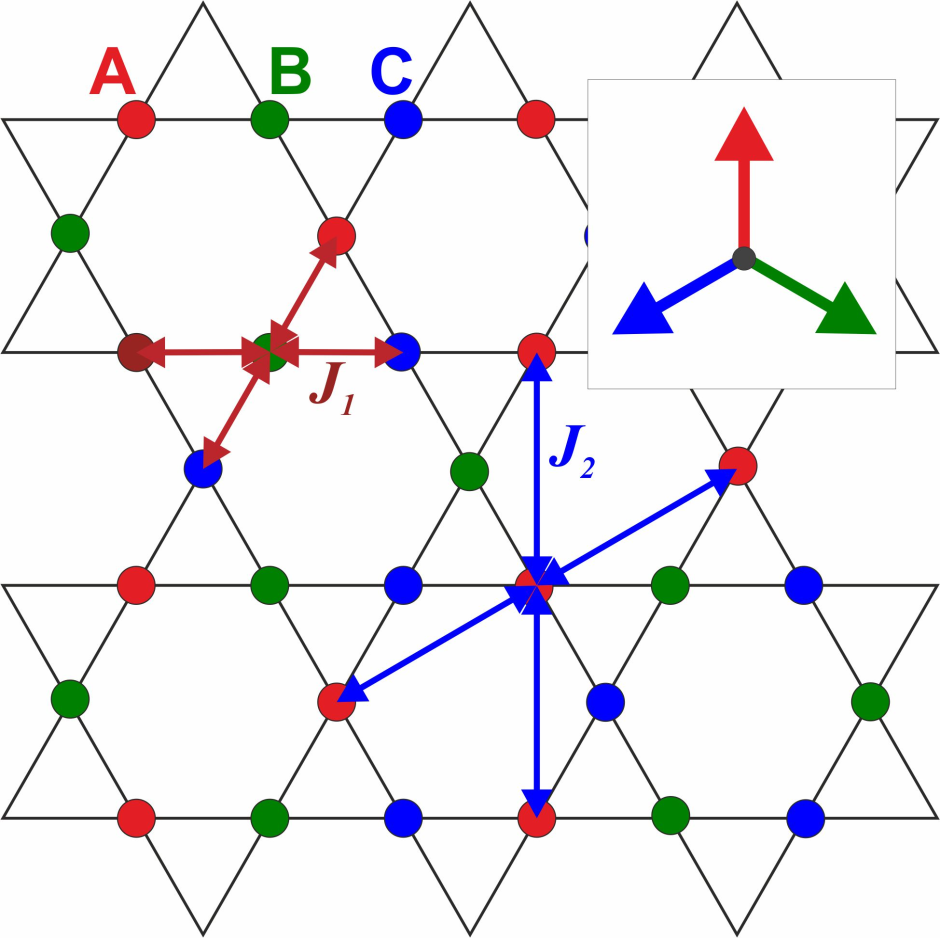
\includegraphics[width=0.4\textwidth]{mma/image2.png}
    \end{center}
    \caption{Модель Поттса с числом состояний спина $q = 3$ на решетке Кагоме.}
    \label{mma-fig-1}
\end{figure}

В данной работе значения обменных интегралов нами были приняты равными: $J_1 = 1$, а $J_2$ было принято антиферромагнитным и менялось по величине от 0 до 2. Таким образом, в исследованной нами в данной работе модели Поттса на решетке Кагоме учитывается ферромагнитное взаимодействие между ближайшими соседями спина и антиферромагнитное взаимодействие разной величины между следующими за ближайшими соседями. Для учета влияния размеров системы на термодинамические свойства исследовались системы с линейными размерами $L=12$ и $L=36$.


\section{Метод исследований}

Исследования проводились на основе алгоритма Ванга-Ландау метода Монте-Карло (МК) \cite{mma-bib-10, mma-bib-11, mma-bib-12, mma-bib-13, mma-bib-14, mma-bib-15}. Данный алгоритм является реализацией метода энтропийного моделирования и его основной особенностью является возможность расчета функции плотности состояний системы, зная которую можно легко вычислить любые интересующие нас термодинамические параметры системы.

Алгоритм Ванга-Ландау является разновидностью энтропийного моделирования и, как показывает опыт его применения в последние годы, является весьма эффективным для исследования различных дискретных спиновых систем \cite{mma-bib-14}.

Алгоритм Ванга-Ландау основан на том, что совершая случайное блуждание в пространстве энергий с вероятностями, обратно пропорциональными плотности состояний $g(E)$, мы получаем равномерное распределение по энергиям. Подобрав вероятности перехода такими, что посещение всех энергетических состояний стало бы равномерным, можно получить изначально неизвестную плотность состояний $g(E)$, зная которую можно вычислить значения необходимых термодинамических параметров при любой температуре. Так как плотность состояний $g(E)$ очень быстро растет с увеличением размеров исследуемых систем, для удобства хранения и обработки больших чисел пользуются величиной $\ln g(E)$.

Важным обстоятельством является то, что плотность состояний $g(E)$ не зависит от температуры, следовательно, рассчитав ее однократно, мы можем вычислить значения любых термодинамических параметров системы при любой ненулевой температуре.

В данной работе нами алгоритм Ванга-Ландау был использован в следующем виде \cite{mma-bib-10, mma-bib-11, mma-bib-12}:
\begin{itemize}
    \item Задается произвольная начальная конфигурация спинов. Стартовые значения плотности состояний $g(E) = 1$, гистограммы распределений по энергиям $H(E) = 0$ и начальное значение модификационного фактора $f = f_0 = e^1 \approx 2.71828$.
    \item Многократно совершаем шаги в фазовом пространстве, пока не получим относительно плоскую гистограмму $H(E)$ (т.е. пока не будут посещены примерно одинаковое количество раз все возможные энергетические состояния системы). В качестве критерия <<плоскости>> гистограммы нами принималось условие отклонения числа посещений всех возможных (с ненулевой плотностью $g(E) \neq 1$) энергетических состояний на величину не более чем на 10\% от среднего значения по системе.
    \item При этом вероятность перехода из состояния с энергией $E_1$ в состояние с энергией $E_2$ определяется по формуле $p = g(E_1)/g(E_2)$. Если переход в состояние с энергией $E_2$ состоялся, то для энергии $E_2$ проводится модификация плотности состояния $g(E_2) \to f \times g(E_2)$, и гистограммы $H(E_2) \to H(E_2) + 1$ иначе меняем параметры для энергии $E_1$ $g(E_1) \to f \times g(E_1)$, $H(E_1) \to H(E_1) + 1$.
    \item Если гистограмма стала <<плоской>> то: обнуляем гистограмму $H(E) \to 0$,  уменьшаем модификационный фактор $f \to \sqrt{f}$, и продолжаем снова и снова, пока модификационный фактор $f \geq f_{\min}$. В качестве минимального значения модификационного фактора нами принималось $f_{\min} = 1.0000000001$.
    \item Каждый раз при достижении энергетического минимума нами проводился анализ магнитной структуры основного состояния и его запись в графический файл. При этом проводилось сравнение полученной конфигурации с ранее полученными и только при обнаружении новой уникальной конфигурации производится ее сохранение в графический файл. Далее данная структура заносится в специальную базу данных для данной модели для дальнейшего сравнения. Данная процедура позволяет избежать дублирования в графических файлах многократно встречающихся состояний с одинаковой магнитной структурой.
    \item После расчета плотности состояний системы для любой интересующей нас температуры рассчитываются различные термодинамические параметры, такие как, энтропия, внутренняя энергия, свободная энергия, теплоемкость, намагниченность, восприимчивость и т.д. Некоторые формулы (\eqref{mma-eq-2}, \eqref{mma-eq-3}, \eqref{mma-eq-4}, \eqref{mma-eq-5}, \eqref{mma-eq-6}), для расчета термодинамических параметров приведены ниже.
    Более подробно алгоритм Ванга-Ландау изложен в работах \cite{mma-bib-10, mma-bib-11, mma-bib-12, mma-bib-13, mma-bib-14, mma-bib-15}.
\end{itemize}

\section{Результаты исследований}

На рисунке \ref{mma-fig-2} приведены значения энергии основного состояния системы при различных значениях взаимодействий $J_1$ и $J_2$. Как видно из графика, в данной модели при низких температурах возможно ферромагнитное упорядочение (FM) (при $J_2 > -0.5$), триплетное антиферромагнитное упорядочение (TAFM) (при $J_2 < -0.5$) или возникновение неупорядоченного фрустрированного состояния ($J_2 = -0.5$).
\begin{figure}[h]
    \begin{center}
        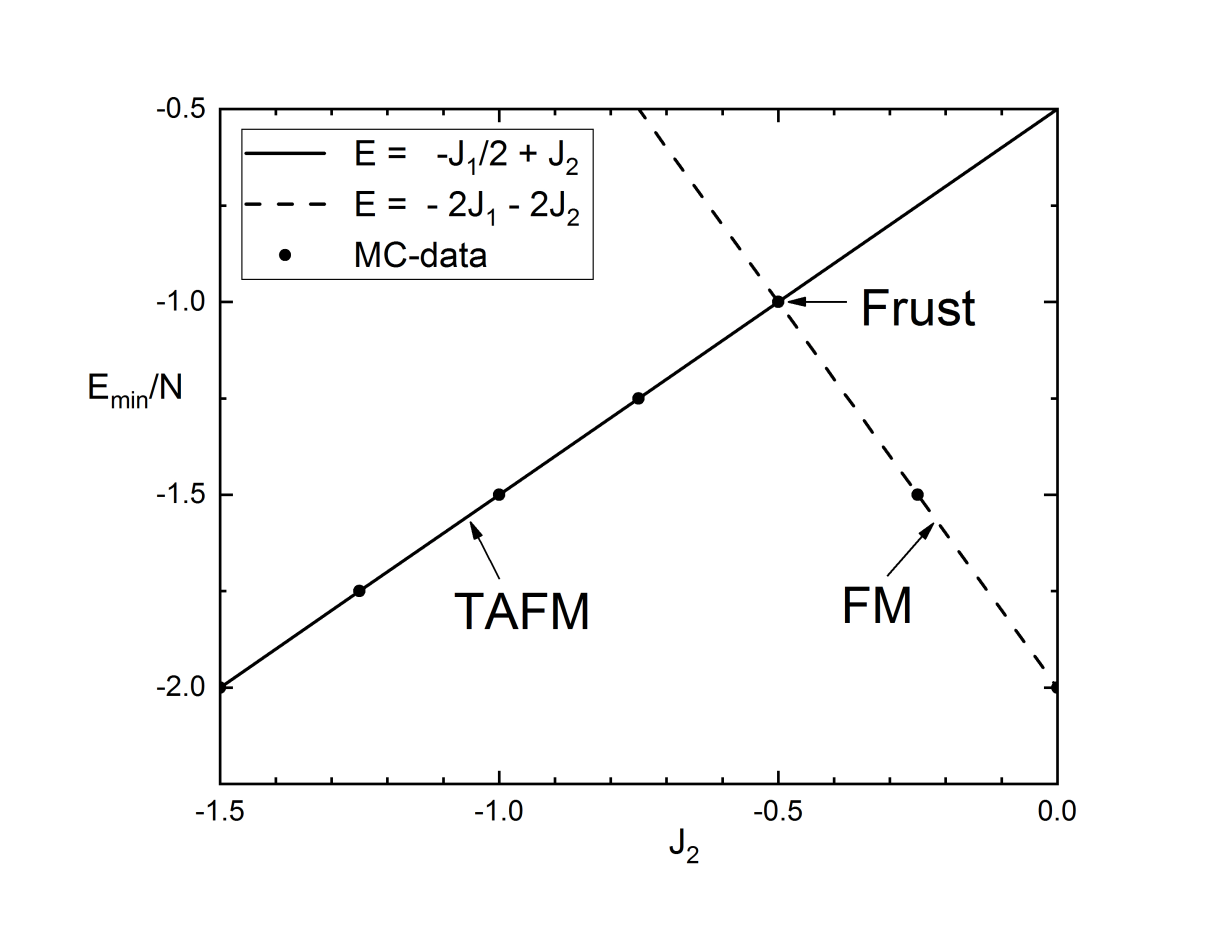
\includegraphics[width=0.5\textwidth]{mma/image19.png}
    \end{center}
    \caption{Энергия основного состояния системы.}
    \label{mma-fig-2}
\end{figure}

Плотность состояний системы $g(E)$ при различных значениях обменных взаимодействий $J_1$ и $J_2$ для систем с линейными размерами $L = 12$ и $L = 36$ приведены на рисунке \ref{mma-fig-3}. На графике приведены плотности состояний для всех трех областей, приведенных на рисунке \ref{mma-fig-2}. Как видно из рисунка, основное состояние системы при $J_2 = -0.5$ сильно вырождено, что обусловлено наличием в данном случае фрустрации в системе, а в остальных случаях вырождение не наблюдается.
\begin{figure}[h]
    \begin{center}
        \begin{subfigure}{0.45\textwidth}
            \begin{center}
                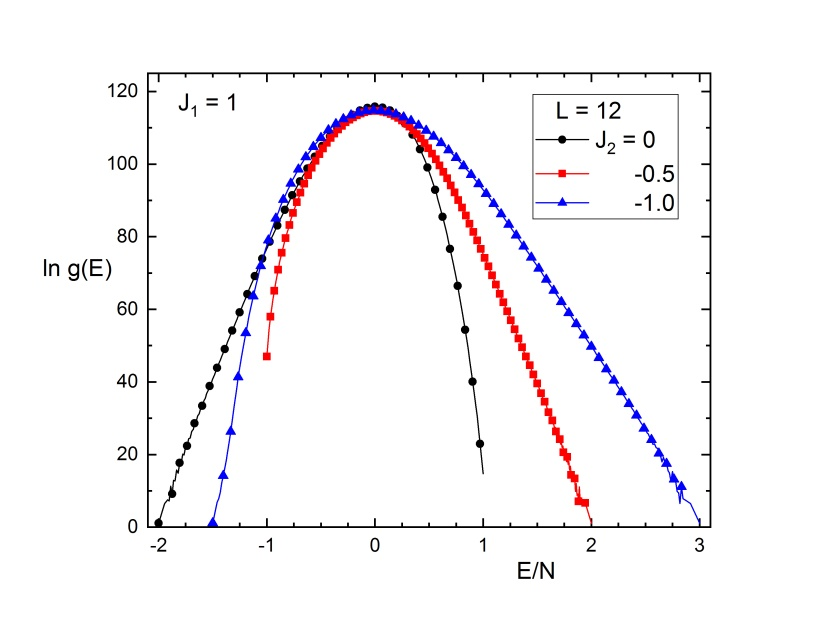
\includegraphics[width=1.0\textwidth]{mma/image20.jpeg}
            \end{center}
        \end{subfigure}
        \begin{subfigure}{0.45\textwidth}
            \begin{center}
                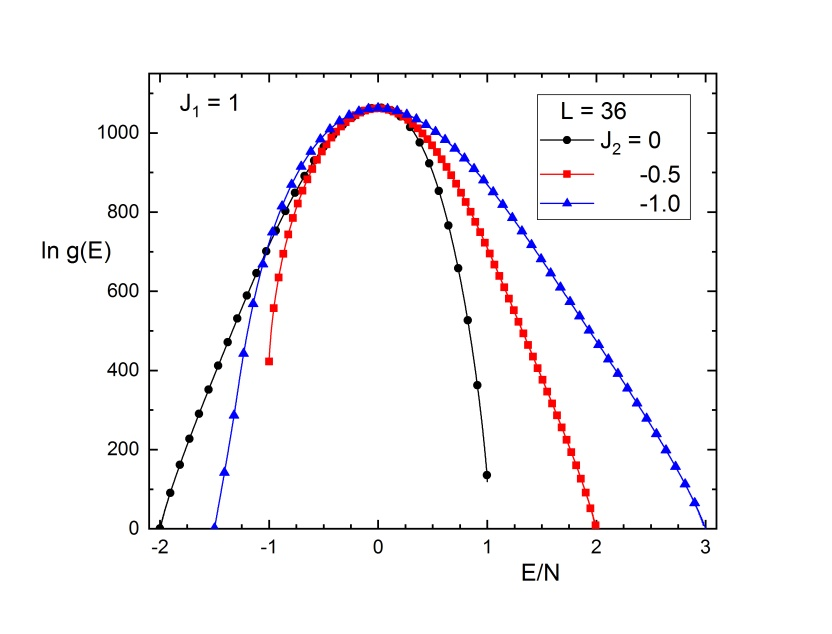
\includegraphics[width=1.0\textwidth]{mma/image21.jpeg}
            \end{center}
        \end{subfigure}
    \end{center}
    \caption{Плотность состояний $g(E)$ для трехвершинной модели Поттса на решетке Кагоме при различных значениях обменных взаимодействий $J_1$ и $J_2$.}
    \label{mma-fig-3}
\end{figure}

На рисунках \ref{mma-fig-4}, \ref{mma-fig-5}, \ref{mma-fig-6} приведены структуры основного состояния для ферромагнитной области ($J_2 > -0.5$), области фрустраций ($J_2 = -0.5$) и триплетной антиферромагнитной области ($J_2 < -0.5$).
\begin{figure}[h]
    \begin{center}
        \begin{subfigure}{0.3\textwidth}
            \begin{center}
                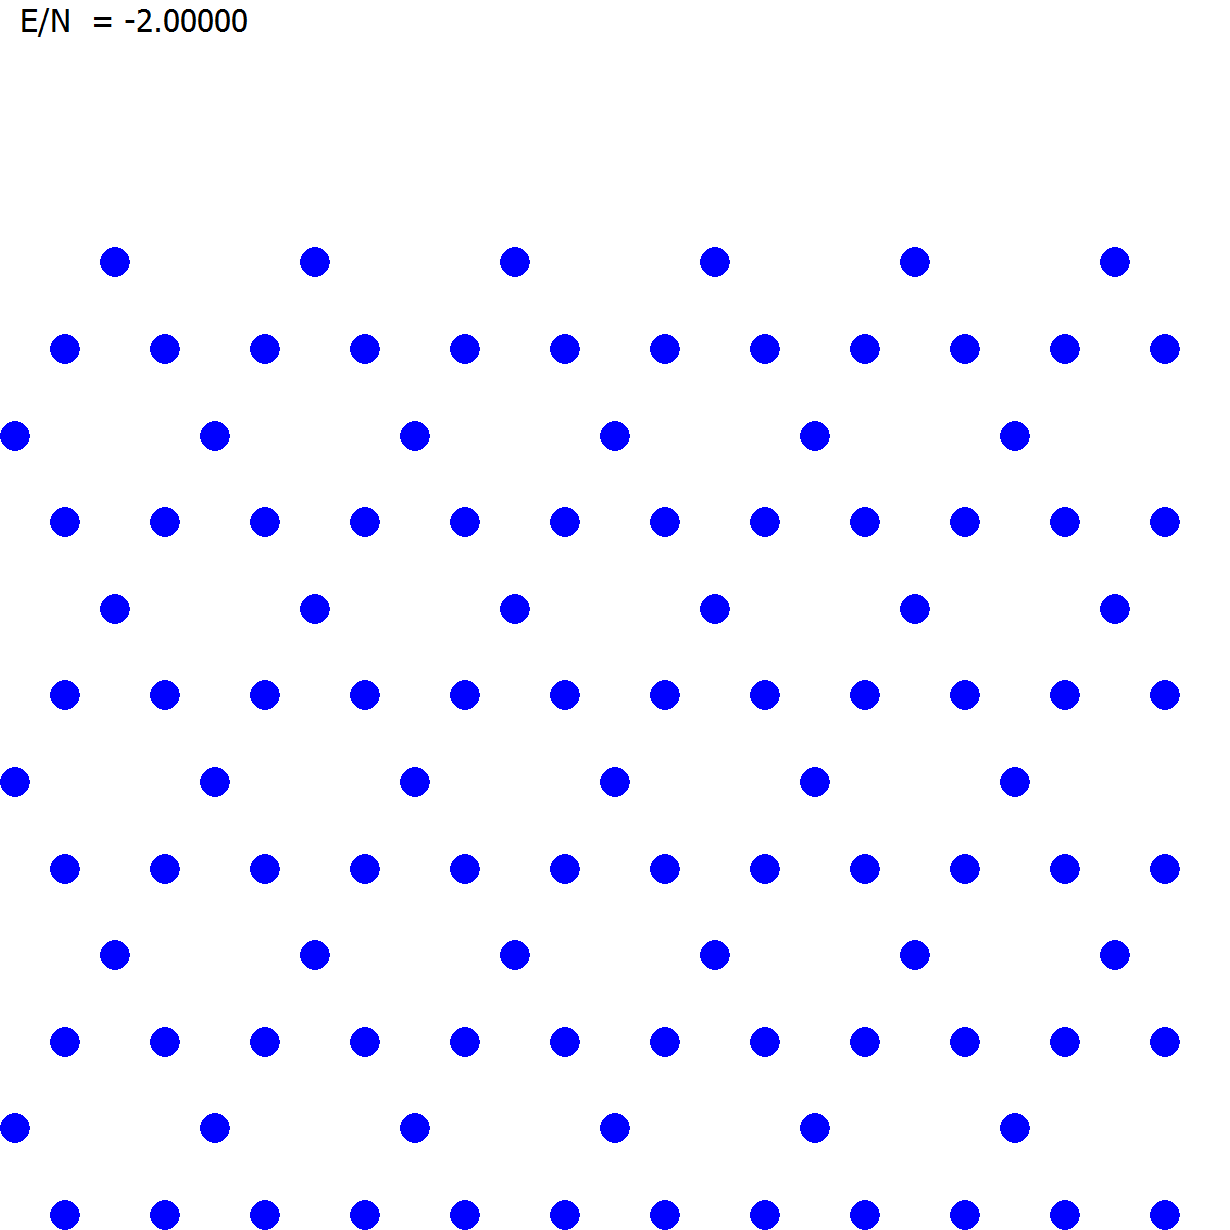
\includegraphics[width=1.0\textwidth]{mma/image24.png}
            \end{center}
            \caption{$J_2 > -0.5$.}
            \label{mma-fig-4}
        \end{subfigure}
        \begin{subfigure}{0.3\textwidth}
            \begin{center}
                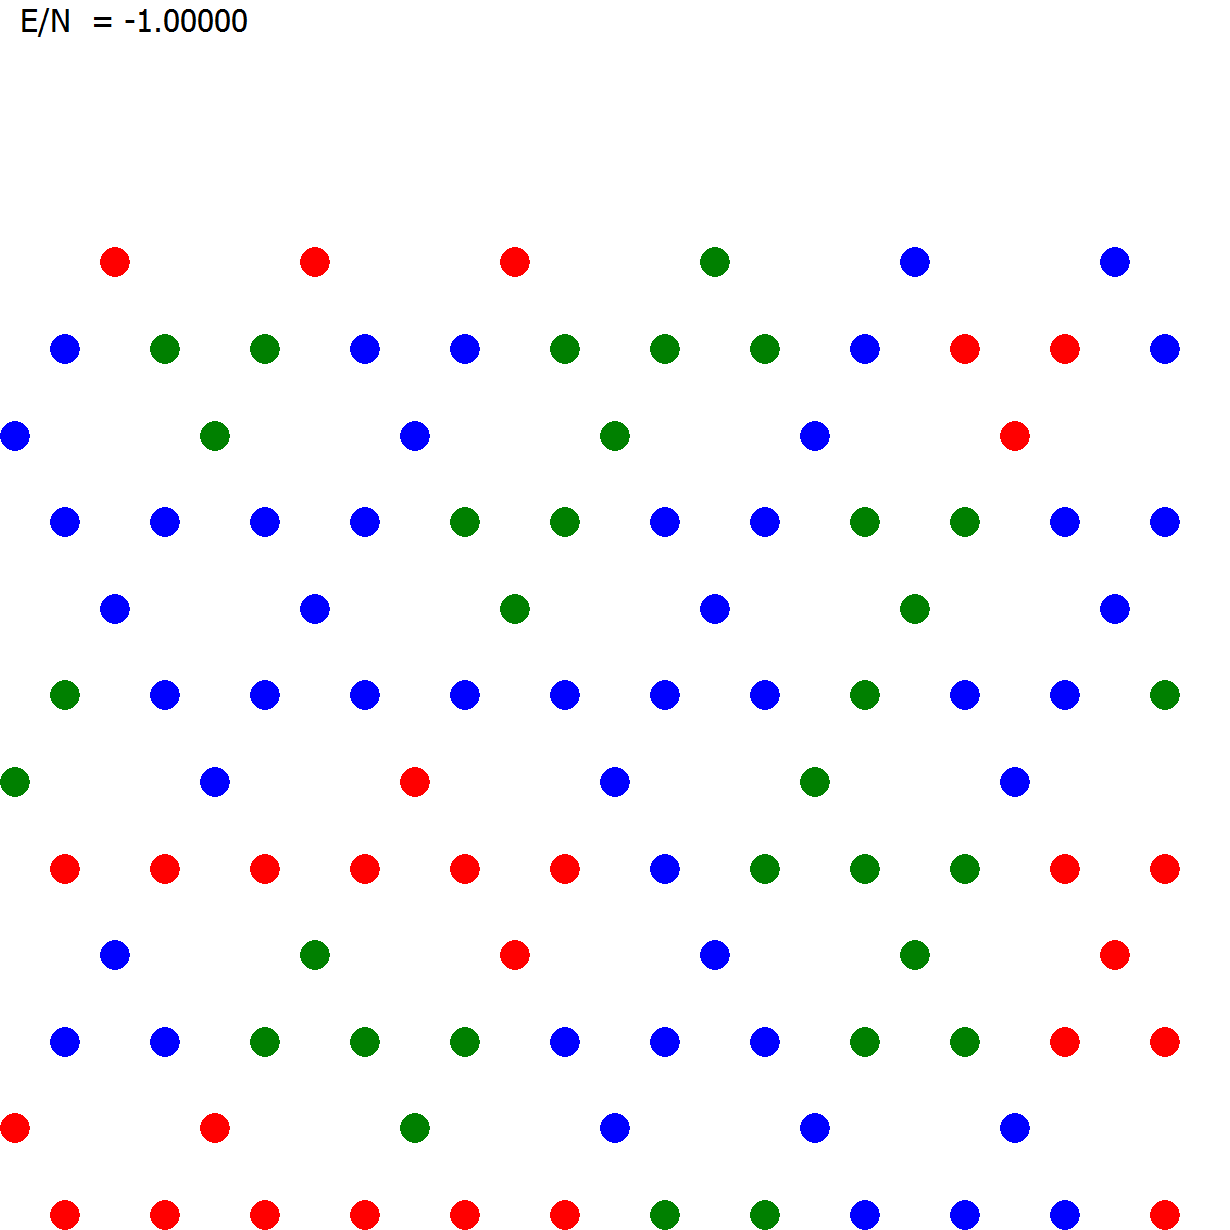
\includegraphics[width=1.0\textwidth]{mma/image25.png}
            \end{center}
            \caption{$J_2 = -0.5$.}
            \label{mma-fig-5}
        \end{subfigure}
        \begin{subfigure}{0.3\textwidth}
            \begin{center}
                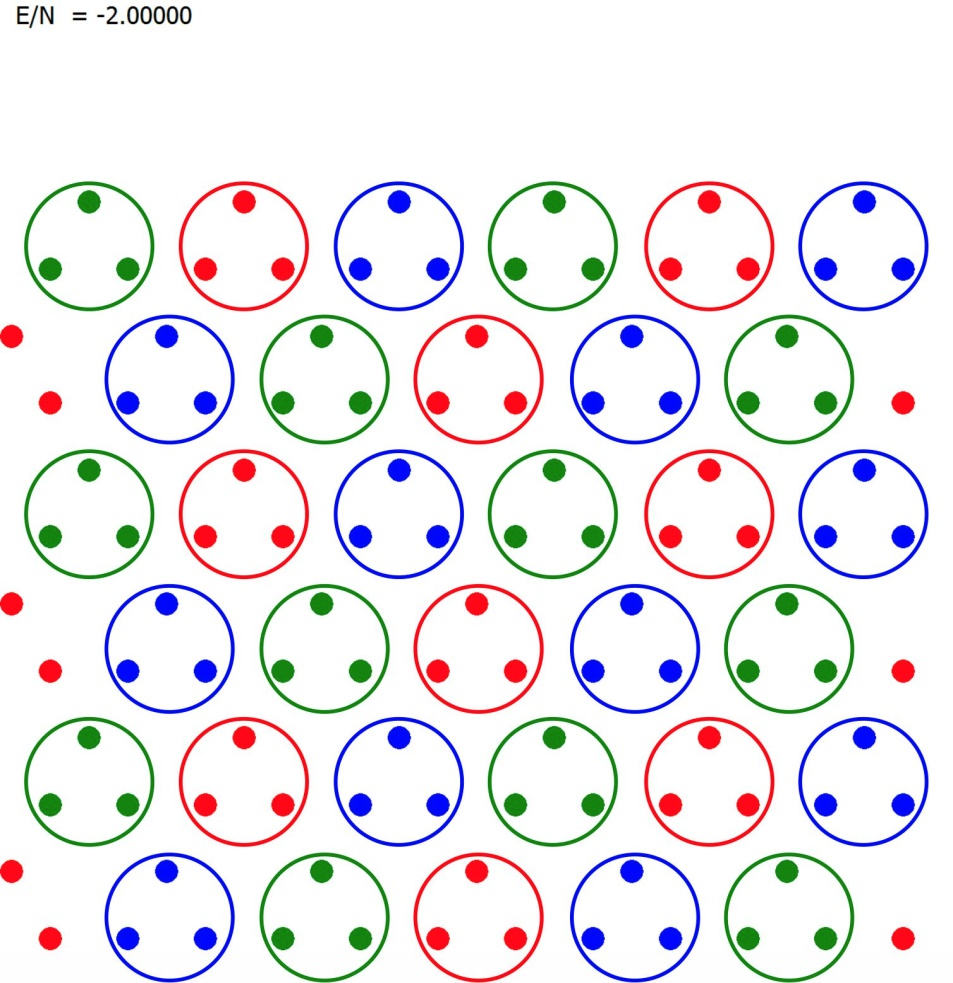
\includegraphics[width=1.0\textwidth]{mma/image26.jpeg}
            \end{center}
            \caption{$J_2 < -0.5$.}
            \label{mma-fig-6}
        \end{subfigure}
    \end{center}
    \caption{Структура основного состояния при разных значениях $J_2$.}
\end{figure}

Энергия основного состояния для ферромагнитной области задается как:
\begin{equation}
    \label{mma-eq-2}
    E_{\min} = -2J_1 - 2J_2.
\end{equation}

Энергия основного состояния для триплетной антиферромагнитной области задается как:
\begin{equation}
    \label{mma-eq-3}
    E_{\min} = - \frac{1}{2} J_1 + J_2.
\end{equation}

Вычислив единожды плотность состояний системы $g(E)$ можно легко рассчитать температурную зависимость любой интересующей нас величины. Например, внутренняя энергия $E$, свободная энергия $F$, и энтропия $S$ системы могут быть рассчитаны следующим образом \cite{mma-bib-14}:
\begin{gather}
    \label{mma-eq-4}
    E(T) = \frac{\sum_{E} Eg(E) e^{-E/k_B T}}{\sum_{E} g(E) e^{-E/k_B T}},
    \\
    \label{mma-eq-5}
    F(T) = -k_B T \ln \left( \sum_E g(E) e^{-E/k_B T} \right),
    \\
    \label{mma-eq-6}
    S(T) = \frac{E(T) - F(T)}{T},
    \\
    \label{mma-eq-7}
    C(T) = \frac{\langle E^2 \rangle - \langle E \rangle^2}{k_B T^2}.
\end{gather}

Рассчитанные из плотности состояний $g(E)$ по формулам \eqref{mma-eq-4}, \eqref{mma-eq-5}, \eqref{mma-eq-6}, \eqref{mma-eq-7} температурные зависимости внутренней энергии E и теплоемкости C при различных значениях обменных взаимодействий $J_1$ и $J_2$, для систем с линейными размерами $L=12$ и $L=36$ приведены на рисунках \ref{mma-fig-7} и \ref{mma-fig-8} соответственно. Отметим важную особенность алгоритма Ванга-Ландау: значения любых термодинамических параметров можно определить для любой температуры, с любым шагом, при этом объем необходимых вычислений, в отличие от других классических алгоритмов метода Монте-Карло, вырастает незначительно.
\begin{figure}[h]
    \begin{center}
        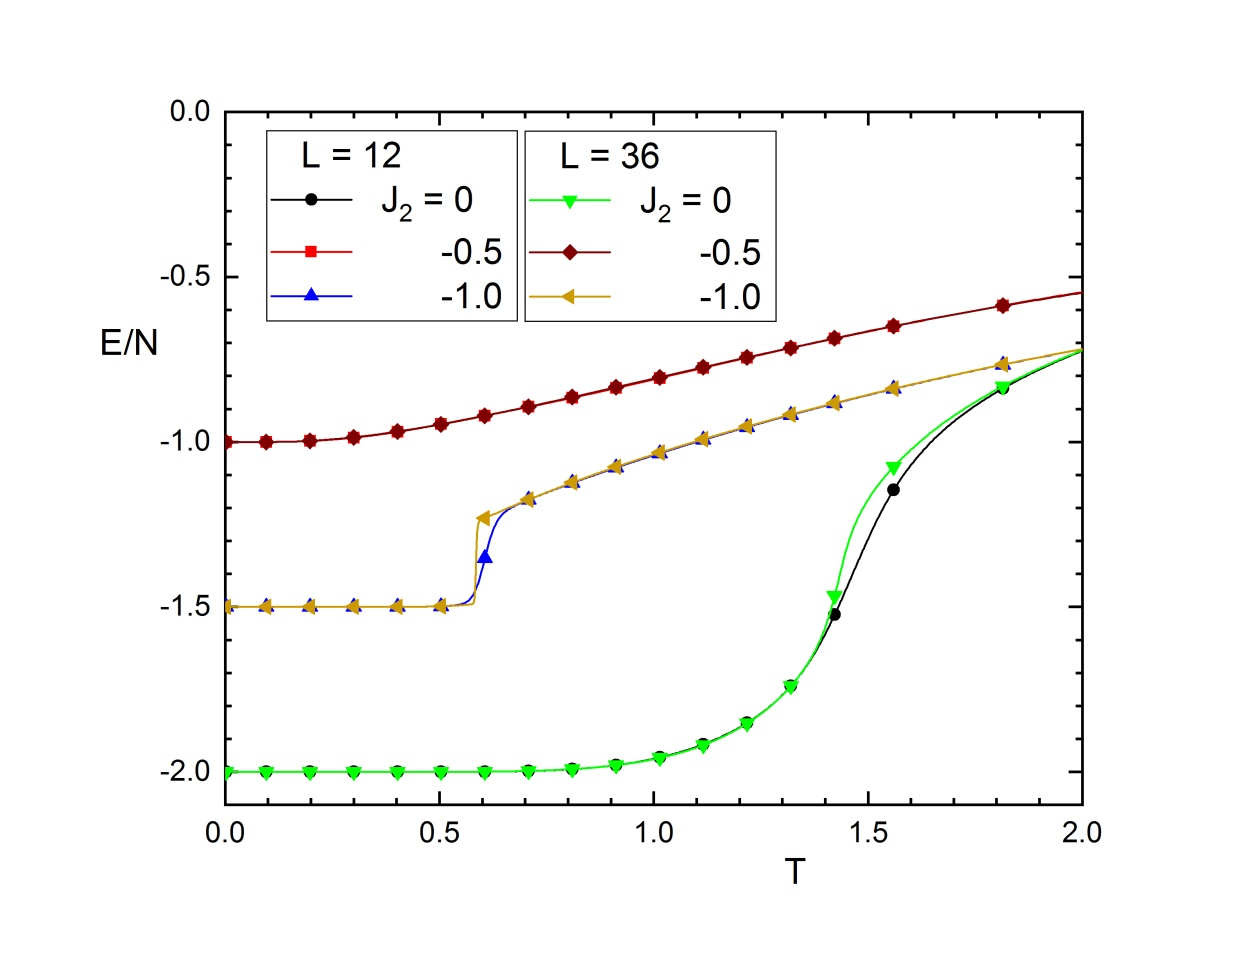
\includegraphics[width=0.5\textwidth]{mma/image31.jpeg}
    \end{center}
    \caption{Температурные зависимости внутренней энергии $E$, рассчитанные из плотности состояний $g(E)$ при различных значениях $J_1$ и $J_2$.}
    \label{mma-fig-7}
\end{figure}
\begin{figure}[h]
    \begin{center}
        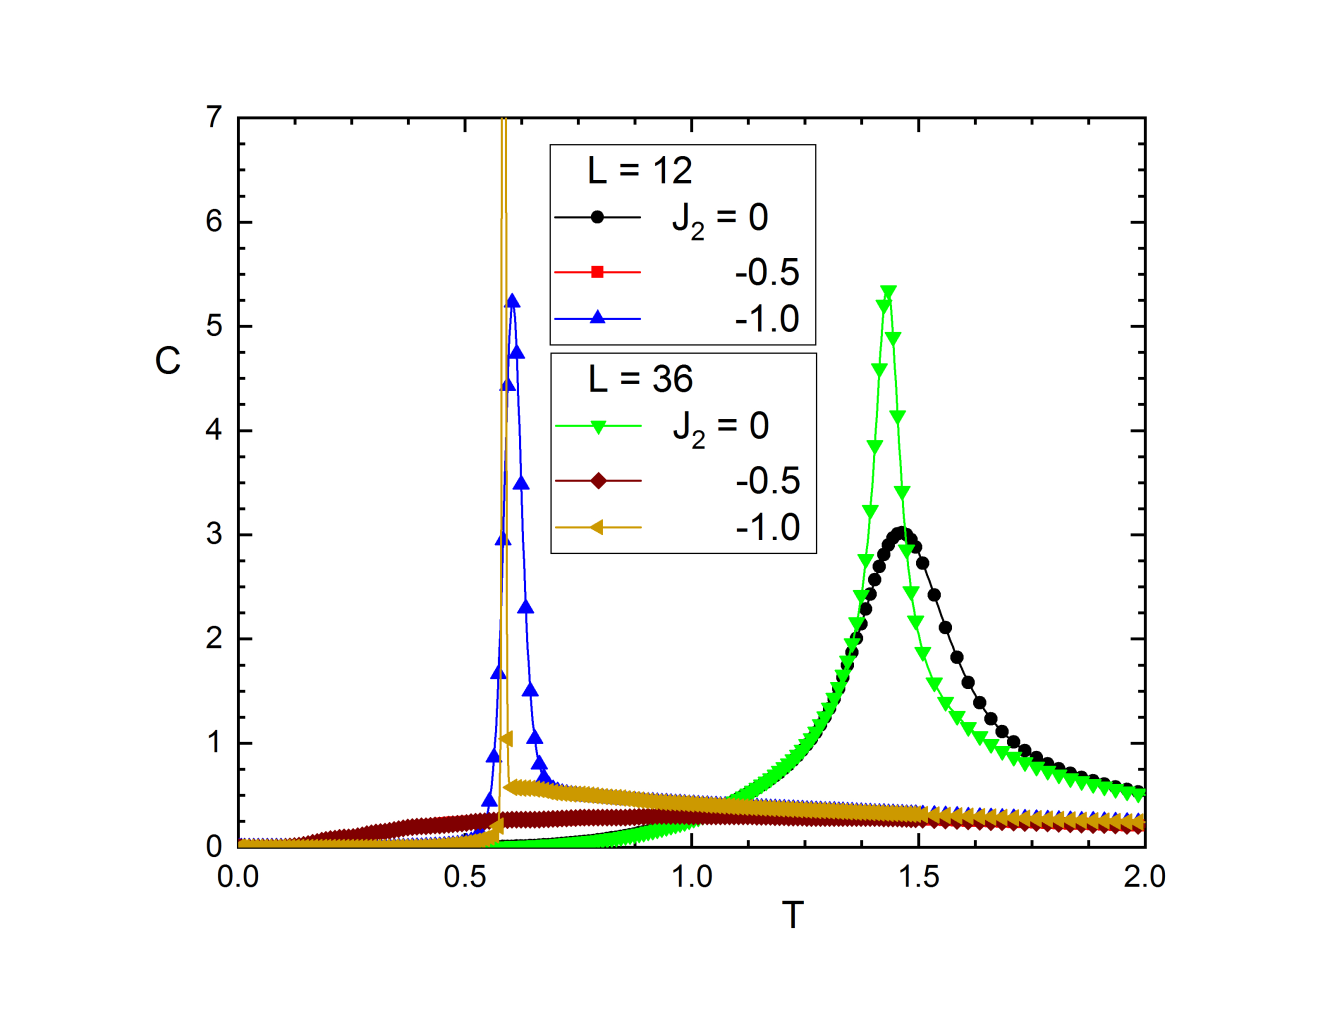
\includegraphics[width=0.5\textwidth]{mma/image32.png}
    \end{center}
    \caption{Температурные зависимости теплоемкости $C$, рассчитанные из плотности состояний $g(E)$ при различных значениях $J_1$ и $J_2$.}
    \label{mma-fig-8}
\end{figure}

Из рисунка \ref{mma-fig-7} видно, что в случае в случае $J_2=-1$ на графике наблюдается энергетический скачок, что говорит о фазовом переходе первого рода. Температурная зависимость теплоемкости, приведенная на рисунке \ref{mma-fig-8}, подтверждает эти предположения. В случае $J_2=-0.5$ скачка теплоемкости не наблюдается, в системе в данном случае не происходит фазового перехода. При $J_2=0$ происходит фазовый переход второго рода.

Для более подробного анализа фазовых переходов и определения типа перехода мы использовали гистограммный метод анализа данных.

Если рассчитать гистограмму по энергии по формуле:
\begin{equation}
    \label{mma-eq-8}
    P(E) = g(E) e^{-E/k_B T}
\end{equation}
то в области фазового перехода мы будем наблюдать два пика для фазового перехода первого рода и один максимум для фазового перехода второго рода.

На рисунке \ref{mma-fig-9} приведены гистограммы энергий в области фазового перхода при $J_2 = -1$ и $J_2 = 0$. Как видно из рисунка при $J_2 = -1$ в системе происходит фазовый переход первого рода, а при $J_2 = 0$ фазовый переход второго рода.
\begin{figure}[h]
    \begin{center}
        \begin{subfigure}{0.45\textwidth}
            \begin{center}
                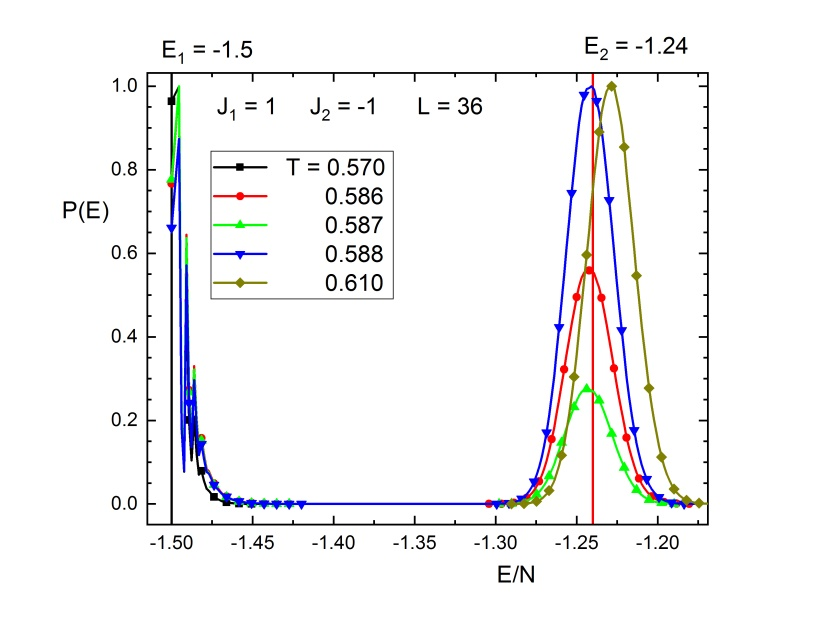
\includegraphics[width=1.0\textwidth]{mma/image34.jpeg}
            \end{center}
        \end{subfigure}
        \begin{subfigure}{0.45\textwidth}
            \begin{center}
                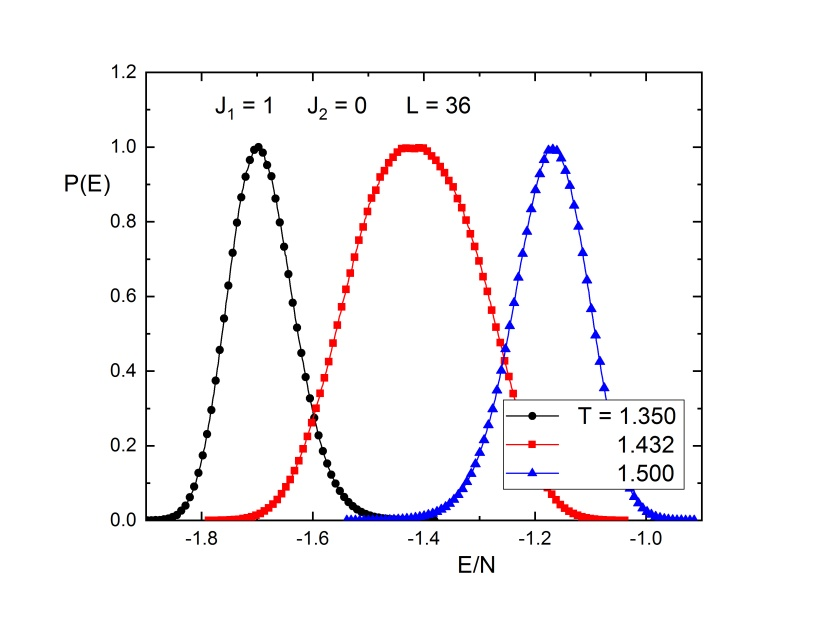
\includegraphics[width=1.0\textwidth]{mma/image35.jpeg}
            \end{center}
        \end{subfigure}
    \end{center}
    \caption{Температурные зависимости энтропии $S$, рассчитанные из плотности состояний $g(E)$ при различных значениях $J_1$ и $J_2$.}
    \label{mma-fig-9}
\end{figure}

Температурные зависимости энтропии $S$ при различных значениях обменных взаимодействий $J_1$ и $J_2$ для систем с линейными размерами $L=12$ и $L=36$ приведены на рисунке \ref{mma-fig-10}. При $J_2 = -0.5$ с понижением температуры энтропия стремится к значению $S_0/N = 0.435$, что говорит о сильном вырождении основного состояния. В остальных случаях с понижением температуры энтропия стремится к нулю. С повышением температуры для всех систем энтропия стремится к значению $\ln3 = 1.09861$.
\begin{figure}[h]
    \begin{center}
        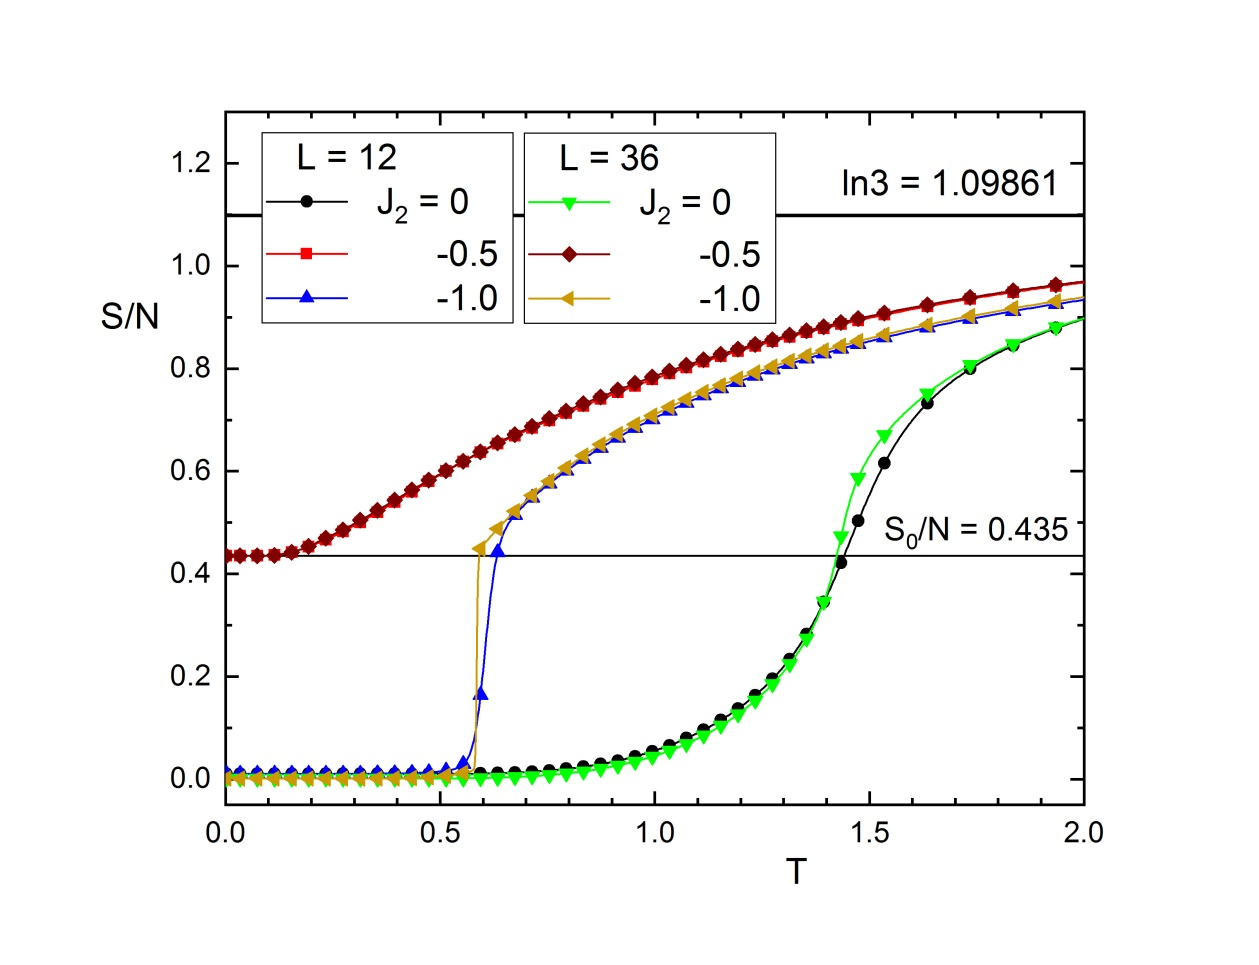
\includegraphics[width=0.5\textwidth]{mma/image36.jpeg}
    \end{center}
    \caption{Температурные зависимости энтропии $S$, рассчитанные из плотности состояний $g(E)$ при различных значениях $J_1$ и $J_2$.}
    \label{mma-fig-10}
\end{figure}

Анализ приведенных выше результатов позволило построить фазовую диаграмму, которая приведена на рисунке \ref{mma-fig-11}.
\begin{figure}[h]
    \begin{center}
        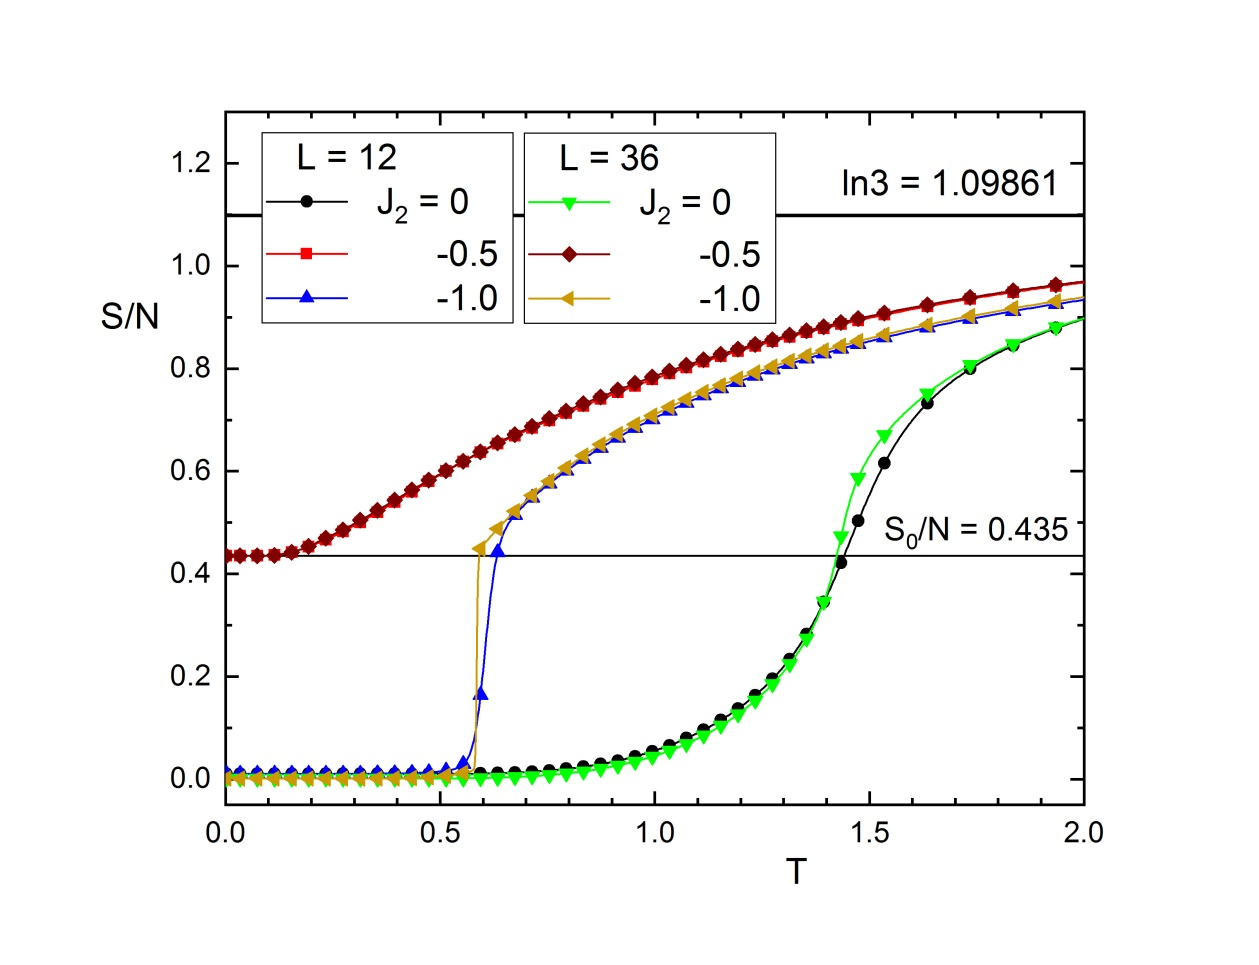
\includegraphics[width=0.5\textwidth]{mma/image36.jpeg}
    \end{center}
    \caption{Фазовая диаграмма.}
    \label{mma-fig-11}
\end{figure}


\section*{Заключение}

Исследование магнитных структур основного состояния, фазовых переходов и термодинамических свойств двумерной модели Поттса с числом состояний спина $q=3$ на решетке Кагоме с учетом взаимодействий первых и вторых ближайших соседей выполнено с использованием алгоритма Ванга-Ландау метода Монте-Карло. Получены магнитные структуры основного состояния в широком интервале значений величины взаимодействия вторых ближайших соседей. Построена фазовая диаграмма зависимости критической температуры от величины взаимодействия вторых ближайших соседей. Для значения $\left| J_2/J_1 = 0.5 \right|$ наблюдается вырождение основного состояния, и система становится фрустрированной.

Таким образом, по проделанной работе можно сделать следующие выводы:
\begin{itemize}
    \item Предложена модель Поттса с числом состояний $q=3$ на решетке Кагоме, учитывающая обменное взаимодействие между первыми и вторыми ближайшими соседями;
    \item Разработана программа для ЭВМ, основанная на новейшем алгоритме Ванга-Ландау, позволяющая исследовать модель Поттса с числом состояний $q=3$ на решетке Кагоме;
    \item Методом Ванга-Ландау вычислены плотности состояний $g(E)$ для модели Поттса с числом состояний $q=3$ на решетке Кагоме.
    \item Определены магнитные структуры основного состояния при различных значениях обменных взаимодействий и показано, что основное состояние может быть ферромагнитным (при $J_2 > -0.5$), триплетным антиферромагнитным (при $J_2 < -0.5$) или сильно вырожденным неупорядоченным фрустрированным (при $J_2 = -0.5$);
    \item Рассчитаны температурные зависимости различных термодинамических параметров, таких как свободная энергия $F$, внутренняя энергия $E$, энтропия $S$, теплоемкость $C$;
    \item Показано, что энтропия для данной модели при температурах близких к абсолютному нулю, при различных соотношениях обменных взаимодействий близка к нулю, кроме случая $J_2 = -0.5$, которое соответствует сильно вырожденному фрустрированному состоянию. С повышением температуры энтропия во всех случаях стремится к теоретически предсказанному значению $\ln 3$;
    \item Вычислены температуры фазовых переходов и определены типы фазовых переходов, происходящих в системе при различных значениях обменных взаимодействий. Построена фазовая диаграмма модели.
\end{itemize}

Результаты, полученные в ходе исследований, могут быть полезными для описания различных низкоразмерных магнитных материалов, имеющих структуру типа решетки Кагоме, таких как Гербертсметиты, Делафосситы, Капелласиты, Фольбортиты и т.д.

\chapter{Влияние магнитного поля на фазовые переходы двумерной модели Поттса с
\texorpdfstring{$q=4$}{q=4} на гексагональной решетке}\label{RMK}


%\section*{Аннотация}
%
%Методом Монте-Карло получены магнитные структуры основного состояния двумерной модели Поттса с числом состояний спина $q = 4$ на гексагональной решетке с учетом взаимодействий первых и вторых ближайших соседей во внешнем магнитном поле $h$. Установлено, что в интервалах значений магнитного поля $0 < h < 1.0$ и $2.0 \leq h \leq 3.5$ наблюдается фазовый переход первого рода, а при значении поля $h = 1.5$ --- фазовый переход второго рода. Показано, что в интервале $4.0 \leq h \leq 7.0$ магнитное поле снимает вырождение основного состояния, и фазовый переход размывается.


\section{Введение}

В течении последних десятилетий наблюдается повышенный интерес к изучению эффектов фрустрации в спиновых решеточных моделях. Конкуренция обменных взаимодействий может привести в магнитных спиновых системах к возникновению фрустрации, которые не позволяют системе одновременно минимизировать все ее локальные взаимодействия, что приводит к бесконечно вырожденному основному состоянию \cite{rmk-bib-1}. Спиновые системы с фрустрациями обладают богатой природой фазовых переходов (ФП) и имеют особенности магнитного, термодинамического и критического поведения. Особый интерес имеет изучение влияния возмущений различной природы, таких как внешнее магнитное поле, взаимодействие вторых ближайших соседей, немагнитные примеси, тепловые и квантовые флуктуации и др. на физические свойства магнитных спиновых систем с фрустрациями. Включение этих возмущающих факторов может привести к совершенно новому физическому поведению таких систем \cite{rmk-bib-2}.

В связи с этим, нами изучается влияние внешнего магнитного поля на характер ФП, магнитные и термодинамические свойства двумерной модели Поттса с фрустрациями. Для фрустрированной модели Поттса существует совсем немного надежно установленных фактов. Большинство имеющихся результатов получены для двумерной модели Поттса с числом состояний спина $q = 2$ и $q = 3$ \cite{rmk-bib-3}. Эта модель изучена достаточно хорошо и получены интересные результаты. Модель Поттса демонстрирует температурный ФП первого или второго порядка, в зависимости от числа состояний спина q, пространственной размерности и геометрии решетки. Двумерная модель Поттса с числом состояний спина $q = 4$ довольно уникальна и до сих пор малоизучена. Результаты исследований двумерной ферромагнитной модели Поттса с числом состояний спина $q = 4$ на треугольной, гексагональной решетках и на решетке Кагоме, полученные методом Монте-Карло (МК) показывают, что в данной модели наблюдается ФП первого рода.

Интерес к модели Поттса обусловлен еще и тем, что эта модель служит основой теоретического описания широкого круга физических свойств и явлений в физике конденсированных сред. К их числу относятся некоторые классы адсорбированных газов на графите, сложные анизотропные ферромагнетики кубической структуры, спиновые стекла, многокомпонентные сплавы и жидкие смеси. На основе модели Поттса с различным числом состояний спина могут быть описаны структурные ФП во многих материалах.

Работ, посвященных изучению влияния внешнего магнитного поля, как возмущающего фактора, на ФП, магнитные и термодинамические свойства модели Поттса с числом состояний спина $q = 4$ практически нет, и этот вопрос все еще остается открытым и малоизученным. В связи с этим, в данной работе нами основе метода МК изучено влияние внешнего магнитного поля на ФП, магнитные и термодинамические свойства двумерной модели Поттса с числом состояний спина $q = 4$ на гексагональной решетке с учетом обменных взаимодействий первых и вторых ближайших соседей. Исследования проводятся на основе современных методов и идей, что позволит получить ответ на ряд вопросов, связанных с характером и природой ФП фрустрированных спиновых систем.


\section{Результат исследования}

Получена фазовая диаграмма зависимости параметра порядка $m$ от величины магнитного поля $h$ в низкотемпературной области (рис. \ref{rmk-fig-1}). На рисунке мы наблюдаем ступенчатую зависимость параметра порядка. Наблюдаются четыре ступеньки: I, II, III и IV. Ступенька I соответствует магнитному упорядочению, при котором только одно состояние спина совпадает с направлением внешнего поля. При увеличении внешнего магнитного поля ($h = 1.5$) еще одно состояние спина выстраивается вдоль внешнего поля. В системе возникает частичный порядок. Это приводит к возникновению ступеньки II на графике. При дальнейшем увеличении поля ($h = 3.0)$, вдоль внешнего поля выстраивается еще одно состояние спина (третье). Этим обусловлено возникновение ступеньки III на графике. При значении поля $h = 4.5$, вдоль внешнего поля выстраивается следующее состояние спина (четвертое). С этим связано возникновение ступеньки IV на графике \cite{rmk-bib-4}.
\begin{figure}[h]
    \begin{center}
        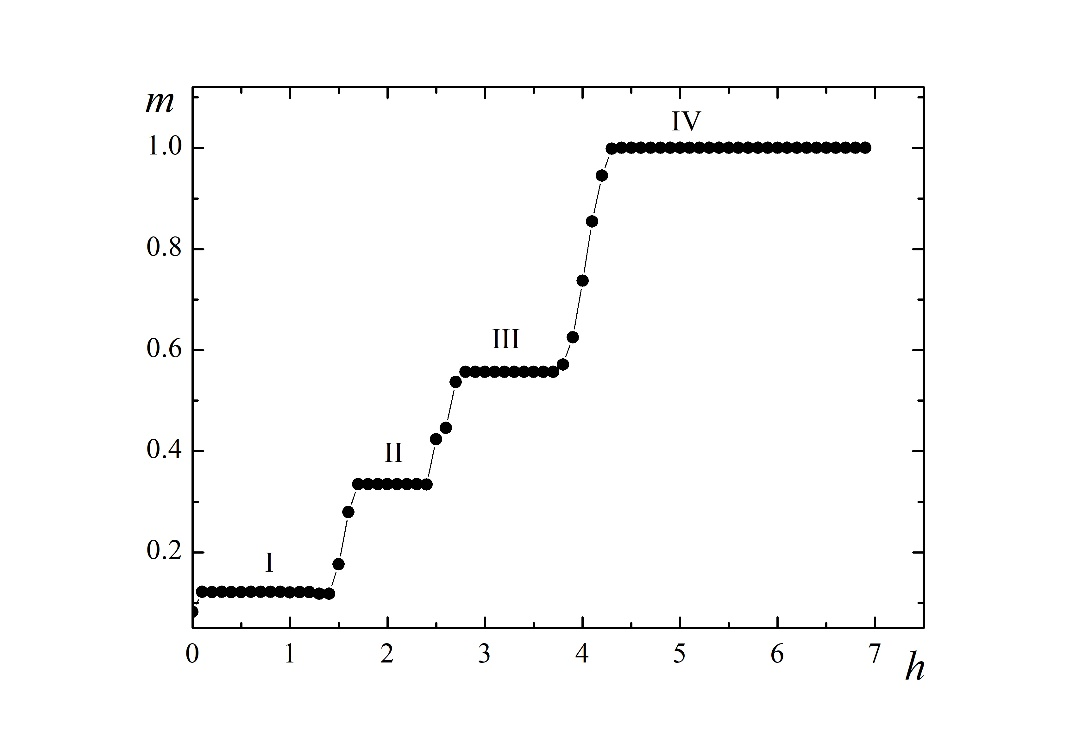
\includegraphics[width=0.75\textwidth]{rmk/image1.jpeg}
    \end{center}
    \caption{Фазовая диаграмма зависимости параметра порядка $m$ от магнитного поля.}
    \label{rmk-fig-1}
\end{figure}

Анализируя рис. \ref{rmk-fig-1} можно предположить, что поля $h = 1.5$; $2.5$ и $4.0$ являются для данной модели фрустрирующими полями. Это также подтверждается поведением температурной зависимости теплоемкости. Теплоемкость в этих полях пологая и значительно ниже, чем в остальных (нефрустрирующих) полях \cite{rmk-bib-4, rmk-bib-5}.


\section*{Заключение}

Исследование влияния магнитного поля на фазовые переходы, магнитные структуры основного состояния и термодинамические свойства двумерной модели Поттса с числом состояний спина $q = 4$ на гексагональной решетке с взаимодействиями вторых ближайших соседей выполнено с использованием репличного обменного алгоритма метода Монте-Карло. На основе гистограммного метода проведен анализ характера фазовых переходов. Получены магнитные структуры основного состояния в широком интервале значений поля. Построена фазовая диаграмма зависимости параметра порядка от величины магнитного поля. Показано, что в интервале значений магнитного поля $0.0 \leq h \leq 3.5$, кроме значения $h = 1.5$ наблюдается фазовый переход первого рода. Для поля $h = 1.5$ наблюдается фазовый переход второго рода. Обнаружено, что при сильных полях $h \geq 4.0$ магнитное поле снимается вырождение основного состояния и фазовый переход в системе размывается.

\chapter{Отчет ведущего научного сотрудника ОМИ ДНЦ РАН 0.5 ст. д.ф.-м.н., проф. Магомедова А.М. за 2022 г.}


%\section*{Аннотация}
%
%Направления работы в 2022 году:
%
%\begin{enumerate}
%    \item Прикладное программирование.
%    \item Проблемы перечислительной комбинаторики.
%    \item Разработка методического, алгоритмического и программного обеспечения.
%\end{enumerate}


\section{Прикладное программирование}

Разработаны или существенно улучшены более двадцати программ прикладного программирования; издана монография и подготовлен черновой вариант  учебного пособия по системе компьютерной математики <<Mathematica>>.


\subsection{Построение алгоритмов. Издание монографии}

Подготовлена и издана монография \cite{akm-bib-m1}, все 20 разделов которой посвящены нестандартным проблемам прикладного программирования (первый рецензент -- Шарапудинов Т.И.).
Основное внимание уделено разработке алгоритмов и обсуждению подходов к решению, не ограничиваясь при решении конкретной задачи одним-единственным алгоритмом; для ряда задач предложены два-три различных алгоритма, воплощенные в одной программе для удобства сравнения по быстродействию; характерной особенностью является многоязычие --- в некоторых программах используется взаимодействие средств двух языков высокого уровня; к некоторым задачам предложены по две программы, написанные на разных языках.
Основное внимание уделено разработке алгоритмов.


\subsection{Разработка программного обеспечения}

Приоритетным направлением явилась разработка программного обеспечения, призванного: а) осуществлять поддержку теоретических исследований по дискретной математике (\cite{akm-bib-m9, akm-bib-m10, akm-bib-m14, akm-bib-m15}); б) решить нестандартные задачи прикладного характера.


\section{Проблемы перечислительной комбинаторики}

Продолжены исследования по вычислительным аспектам димерных чисел. Найдено простое доказательство существования прямого рекуррентного соотношения для последовательности димерных чисел прямоугольной полосы при произвольно фиксированной ширине полосы. Усовершенствован алгоритм проверки существования интервальной раскраски у двудольного графа заданного порядка (известная NP-полная задача).


\subsection{Димерные числа}

В 2022 г. одним из основных направлений нир явилось продолжение исследования проблемы димерных чисел, другими словами, -- задачи вычисления числа $T(m,n)$ совершенных паросочетаний в решёточном графе заданных размеров $m\times n$. Известно, что $T(m,n)$ равно числу всевозможных разбиений прямоугольной полосы $m\times n$ на плитки $1\times 2$. При фиксированной ширине $m$ принято обозначать $T(m,n)$ через $a_n$. Все известные из литературы прямые рекуррентные соотношения для $a_n$ (т.е. представление $a_n$ в виде линейной комбинации $a_0, a_1,..., a_{n-1}$ с целыми постоянными коэффициентами) получены исходя из того, что факт существования таких прямых рекуррентных соотношений априори известно.

В 2022 г. найдено непосредственное и краткое доказательство данного факта. Это основной результат за 2022 г.

Отметим второй результат в данном направлении. Все полученные ранее рекуррентные соотношения для
$a_n$ (при фиксированном $m$) выводились с использованием двухступенчатой схемы: сначала формировалась система взаимно рекуррентных формула (с.в.р.ф.) для $a_n, b_n, c_n, \dots$ (где $b_n, c_n, ...$  --- димерные числа для фигур, полученных из исходного прямоугольника удалением некоторых клеток верхней строки), затем из с.в.р.ф. методом исключения находили $a_n$ (см., например, \cite{akm-bib-m3}). В текущем году удалось получить рекуррентное соотношение для $a_n$ без использования двухступенчатой схемы (однако распространить результат на $m>4$ не удалось).

\underline {Прикладное значение}. Изучение ряда свойств химического соединения можно эффективно проводить, исследуя топологическую модель молекулы, т. е. представляя молекулу в виде неориентированного графа, в котором вершины соответствуют атомам, а ребра — химическим связям;
некоторые классы химических соединений успешно синтезируются только тогда, когда графы соединений имеют совершенное паросочетание;
компоненты некоторых семейств соединений тем стабильнее, чем больше совершенных паросочетаний в их графах.
	
Задача возникает и при исследовании адсорбции двухатомных молекул на поверхности: требуется найти число способов объединения атомов в двухатомные молекулы (димеры), так чтобы при этом покрывалась дважды периодическая решётка с шагом, равным длине димера, причём каждый димер покрывал бы две смежные точки решётки и не оставалось бы ни одной непокрытой точки.


\subsection{Интервальная раскраска двудольных графов}

Разработанный ранее для проверки существования у двудольного графа  интервальной раскраски алгоритм усилен фрагментом, названным
<<Методом $c$-увеличивающего пути>>. Приведем его краткое описание, где через $LC[v_k]$ обозначен интервал цветов, представленных в вершине $v_k$, через $C[i_k]$ -- цвет ребра с номером $i_k$.

Вершинно-непересекающийся путь из чередующихся ребер (не окрашено -- окрашено в цвет $c$, не окрашено --- окрашено в цвет $c$ -…-  не окрашено):
$$v_1-v_2-v_3-\dots-v_d$$
будем называть <<c-увеличивающим>>, если цвет $с$ является граничным для интервалов $LC[v_1]$ и $LC[v_d] $ и входит в интервалы цветов всех внутренних вершин пути: $v_2,v_3, \dots, v_{d-1}$.
Номера последовательных ребер c-увеличивающего пути обозначим $i_1, i_2, \dots, i_{d-1}$ и выполним действия, увеличивающие число окрашенных ребер пути с сохранением цветов всех ребер, не принадлежащих данному пути:

окрасим ребро $(v_1,v_2)$ в цвет $c$ и удалим цвет ребра $(v_2,v_3)$, окрасим ребро $(v_3,v_4)$ в цвет $c$ и т.д.:

$C[i_1 ]=c, LC[v_1].Add(c);$

$C[i_2]=-1; C[i_3]=c; C[i_4 ]=-1; C[i_5 ]=c; \dots ,C[i_{d-2}]=-1;$

$C[i_{d-1}]=c; LC[d].Add(c)$.

Усиленный описанным методом алгоритм (в реализации \cite{akm-bib-m14, akm-bib-m15}) легко справился с задачей нахождения интервальной раскраски у графа на рис.~\ref{akm-fig-1}. На рисунке вторые метки ребер --- номера цветов.
\begin{figure}[h]
    \begin{center}
        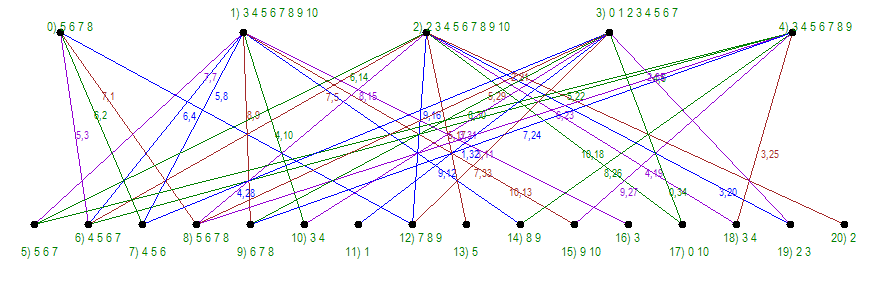
\includegraphics[width=1.0\textwidth]{akm/int.png}
    \end{center}
    \caption{Интервальная раскраска двудольного графа порядка 21, найденная программой. Первая метка ребра -- его номер, вторая метка -- номер цвета ребра. Около каждой вершины 0), 1), ..., 20)  указан список цветов, представленных в данной вершине.}
    \label{akm-fig-1}
\end{figure}

\underline{Прикладное значение.} Интервальная раскраска двудольного графа $(X,Y,E)$ является графической интерпретацией беспростойного расписания мультипроцессорной системы,  где $X$ -- процессоры, $Y$ -- задания, $(x,y) \in E$ если и только если процессору $x$ предписано обработать задание $y$.


\subsection{Симплициальные комплексы заданного типа}

Ранее в соавторстве с Лавренченко C. А.  была опубликована статья, где вводится новый перечислительный многочлен для абстрактных комплексов заданного типа, например, деревьев с фиксированным числом вершин или триангуляции тора с фиксированным графом.
Дальнейшее развитие идей статьи (в направлении исследования свойств вычислительного многочлена) опубликовано в качестве главы 8 в монографии \cite{akm-bib-m3}.


\section{Разработка методического, алгоритмического и программного обеспечения}

Разработаны (в некоторых случаях значительно доработаны частично разработанные ранее программы) и зарегистрированы в гос.реестре программы для ЭВМ, предназначенные для решения перечислительных проблем дискретной математики, компьютерной графики и создания демонстрационного материала по дисциплинам компьютерных наук.


\subsection{Поиск с масштабируемым контекстом в произведениях на языке народа Дагестана (на примере аварского языка)}
\begin{figure}[h]
    \begin{center}
        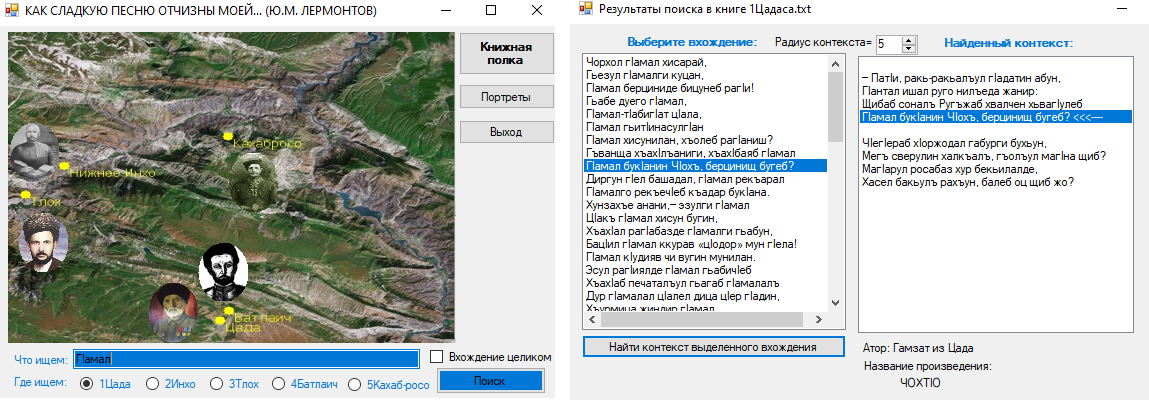
\includegraphics[width=1.0\textwidth]{akm/lit.png}
    \end{center}
    \caption{Поиск с масштабируемым контекстом.}
\end{figure}

Функциональность: а) выбор и отображение литературного произведения для гипертекстового просмотра в окне из трех фреймов: в верхнем - список авторов, в левом фрейме - список ссылок - названий произведений выбранного автора, в правом фрейме выводится текст соответствующего произведения;
б) устойчивый к нечеткости набора поиск наименования произведения и фамилии автора по заданному фрагменту текста.


\subsection{Визуальное восприятие дискретных серий сигналов}

Разработана C\#-программа с существенным повышением надежности разработанного ранее программного обеспечения (на Delphi) для оцифровки серий дискретных звуковых сигналов.

Перспективы: а) анализ программной оцифровки изображения в окне редактора звуков;
б) разработка программы для отображения на экране буквы выполнением 2-серийной дискретной последовательности движений глазами; в) усиление функциональности программы до вывода на экран текста в результате выполнения серий дискретных движений глазами.

\underline{Ожидаемое применение.}
Для общения с обездвиженным пациентом;  в ежедневном быту лиц со слабым слухом.
\begin{figure}[h]
    \begin{center}
        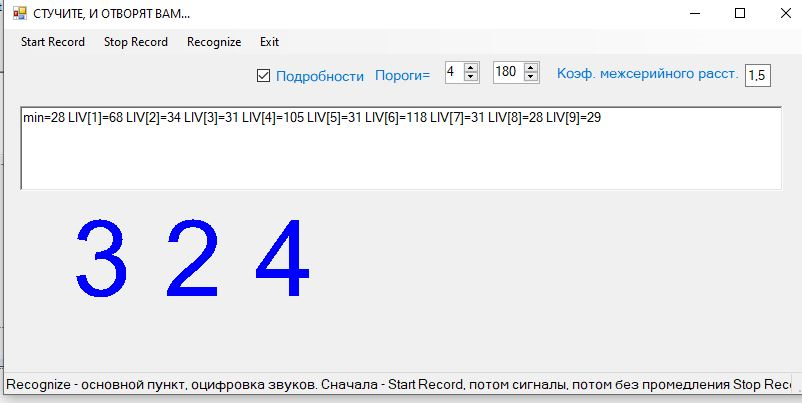
\includegraphics[width=1.0\textwidth]{akm/audio.png}
    \end{center}
    \caption*{Визуальное восприятие дискретных серий сигналов.}
\end{figure}


\subsection{Создание карты Республики Дагестан}

Цели проекта: - разработка 2-мерной муниципальной карты РД с масштабированием и детализацией актуальной местности; поиском населенных пунктов; границ районов; маршрутов; подробной текстовой и графической информацией о выбранном районе или населенном пункте; - частичное решение задачи разработки 3-мерной физической карты РД.
\begin{figure}[h]
    \begin{center}
        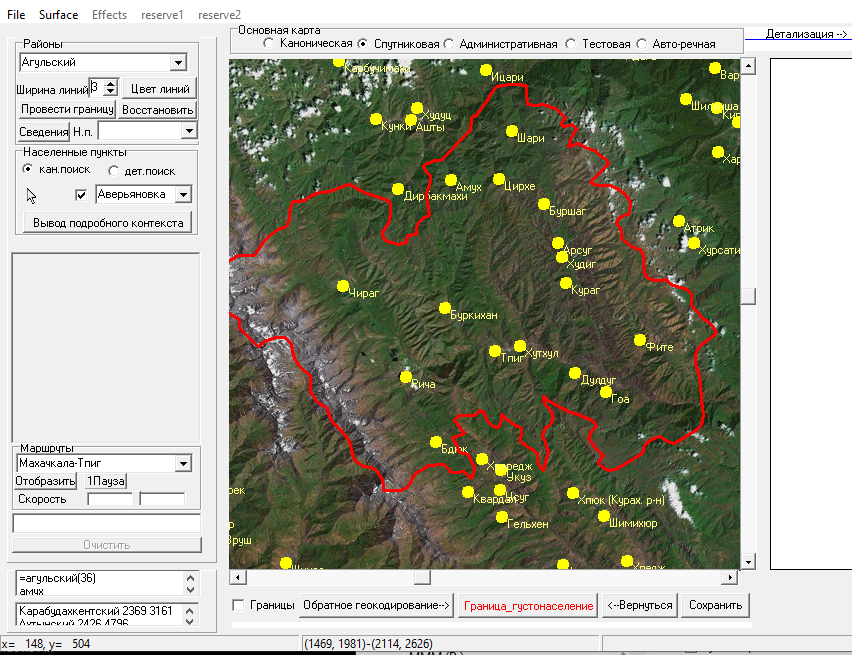
\includegraphics[width=1.0\textwidth]{akm/RDmap.png}
    \end{center}
    \caption*{Создание карты Республики Дагестан.}
\end{figure}
\underline{Примеры пунктов, завершенных к настоящему времени}: <<бесшовное>> склеивание электронной карты РД из отсканированных фрагментов,
просмотр карты значительных размеров путем прорисовки в окне просмотра лишь востребованного в текущий момент фрагмента малых размеров $(512\times 512)$; способы указания в интерактивном режиме выбранного населенного пункта (н.п.): из локального списка названий н.п. текущего района и/или из глобального списка, вводом названия в редактируемое поле или визуальным указанием на карте.


\subsection{Реставрация рукописи}

Программа предназначена для распознавания точек на изображении рукописи: а) фона и б) текста. Цель и задачи программы: замена зашумленного фона рукописного текста однородным или выбранным пользователем фоном, изменение толщины и цвета текста.
Программу рекомендуется использовать для реставрации старых рукописей.

\begin{figure}[h]
    \begin{center}
        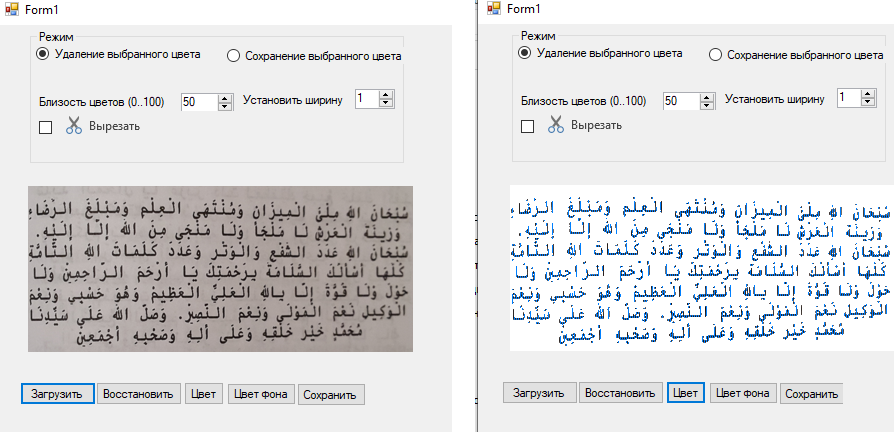
\includegraphics[width=1.0\textwidth]{akm/arab.png}
    \end{center}
    \caption*{Реставрация рукописи. Слева -- исходный рисунок, справа -- результат работы программы.}
\end{figure}


%\section{Заключение}
%
%За 2022 г.  издана монография, опубликованы  в изданиях из списка ВАК  четыре статьи, еще две публикации в сборнике трудов Всероссийской конференции, получены восемь свидетельств о государственной регистрации в Реестре программ для ЭВМ, а также опубликована глава в монографии зарубежных авторов. В 13 из 16 публикаций (а также приравненных к ним) указано, что они выполнены благодаря поддержке ОМИ ДФИЦ РАН.

\chapter{Тема основной части отчета сотрудника}


%\section*{Аннотация}
%
%Была предпринята попытка ослабить условия базисности системы полиномов Лежандра в пространствах Лебега с переменным показателем. Были получены оценки и представления для ядра, играющего важную роль при изучении вопроса базисности данной системы.


%\section*{Введение}
%
%Интерес к пространствам Лебега с переменным показателем $L^{p(\cdot)}$ возрос с 1990-х годов ввиду
%их использования в различных приложениях. Прежде всего, это математические
%моделирование электрореологических жидкостей. Эти пространства также использовались для моделирования поведения других физических явлений, а также для изучения процессов обработки изображений и т. д. Эти задачи, в свою очередь, приводят к поиску систем, образующих базисы в этих пространствах. В работах И.И. Шарапудинова и его учеников \cite{tad-SHII-Haar,tad-SHII-AnalisysMath,tad-SHII-Leg,tad-MMG-Haar,tad-SHII-Jacob,tad-SHII-Ult,tad-RAM-Jacob} была показана базисность в $L^{p(\cdot)}$  тригонометрической системы, системы полиномов Якоби и системы функций Хаара при определенных условиях на показатель $p(x)$.
%
%В отчетном году была предпринята попытка ослабить эти условия на переменный показатель $p(x)$ (постоянство показателя на концах отрезка $[-1,1]$) в случае системы полиномов Лежандра. При исследовании этой задачи возникла необходимость изучения свойств ядра $K(x,y)$, связанного с ядром Кристоффеля -- Дарбу для системы полиномов Лежандра. А именно для $K(x,y)$ получены  представления и оценки, в зависимости от расположения $x,y$ на квадрате $[-1,1]\times[-1,1]$.


\section{О базисности системы полиномов Лежандра в пространствах Лебега с переменным показателем}

Исследован вопрос базисности системы полиномов Лежандра в пространствах Лебега с переменным показателем с целью устранения условия постоянства переменного показателя на концах отрезка $[-1,1]$.


\subsection{Введение}

Пусть $p(x)$ -- неотрицательная измеримая функция, $E=[-1,1]$. Множество функций $f$ таких, что
\begin{equation}\label{s2-lpx-def-1}
  \int_{E}|f(x)|^{p(x)}dx<\infty,
\end{equation}
обозначим через $L^{p(\cdot)}(E)$ и назовем пространством Лебега с переменным показателем. Положим $p_+(E)=ess\sup_{x\in E} p(x)$ и и $p_-(E)=ess\inf_{x\in E} p(x)$. При условии $1\le p_-\le p(x)\le p_+<\infty$ пространство $L^{p(\cdot)}(E)$ нормируемо \cite{tad-lpxtopology} и одну из эквивалентных норм можно задать следующим образом
\begin{equation}\label{s2-lpx-norm}
  \|f\|_{p(\cdot)}=\|f\|_{p(\cdot)}(E)=\inf\left\{\lambda>0:\int_{E}\left|\frac{f(x)}\lambda\right|^{p(x)}dx\right\}.
\end{equation}
Отметим некоторые свойства этих пространств, которые понадобятся в дальнейшем. Пусть $1\le p(x)\le q(x)\le q_+(E)<\infty$. Тогда \cite{tad-SHII-Haar} $L^{q(\cdot)}(E)\subset L^{p(\cdot)}(E)$ и для $f\in L^{q(\cdot)}$
\begin{equation}\label{LpxLqxNormIneq}
  \|f\|_{p(\cdot)}\le r_{p,q}\|f\|_{q(\cdot)},
\end{equation}
где $r_{p,q}=\frac1{\mu_-(E)}+\frac1{\mu'(E)}$ ($\mu(x)=q(x)/p(x)$, $\frac1{\mu(x)}+\frac1{\mu'(x)}=1$).
Если $p(x)>1,\, x \in A$ (не исключая и случай, когда $p_-(A)=1$), то справедливо неравенство типа Гёльдера для пространств Лебега с переменным показателем~\cite[нер-во (8)]{tad-lpxtopology}:
\begin{equation}\label{LpxHoelderIneq}
  \int\limits_A |f(x)||g(x)|dx \le
  C(p,A) \cdot \|f\|_{p(\cdot)}(A) \cdot \|g\|_{p'(\cdot)}(A),
\end{equation}
где $\frac{1}{p(x)}+\frac{1}{p'(x)}=1$, $C(p,A)\le \frac{1}{\underline{p}(A)}+\frac{1}{\underline{p}'(A)}$.
Для любых измеримых множеств $A\subset B$ справедливо неравенство
\begin{equation}\label{LpxNormSubsetIneq}
  \|f\|_{p(\cdot)}(A) \le \|f\|_{p(\cdot)}(B).
\end{equation}
Основополагающую роль в теории пространств Лебега с переменным показателем играет условие Дини -- Липшица
\begin{equation}\label{DiniLipCond}
	|p(x)-p(y)| \le \frac{C}{|\log |x-y||};\ x,y \in E.
\end{equation}


Приведем теперь некоторые сведения о полиномах Лежандра $P_n(x)$, которые нам понадобятся в дальнейшем. Эти полиномы определим при помощи формулы Родрига
\begin{equation}\label{RodrigueFormula}
  P_n(x)=\frac{(-1)^n}{2^nn!}\{(1-x^2)^n\}^{(n)}.
\end{equation}
Для полиномов Лежандра имеет место следующее соотношение ортогональности
\begin{equation}\label{LegOrthRel}
  \int_{-1}^1P_n(x)P_m(x)dx=\frac{2}{2n+1}\delta_{nm},
\end{equation}
где $\delta_{nm}$ -- символ Кронекера. Имеют место следующие свойства полиномов Лежандра
\begin{equation}\label{Leg-Prop1}
  |P_n(x)|\le1,\ x\in[-1,1],
\end{equation}
\begin{equation}\label{Leg-Prop2}
  (1-x^2)^{\frac14}n^{\frac12}|P_n(x)|\le\sqrt{\frac2\pi}.
\end{equation}
\begin{equation}\label{Leg-Prop3}
  (1-x^2)^{\frac14}(n+1)^{\frac12}|P_n(x)-P_{n+2}(x)|\le c\ x\in[-1,1],
\end{equation}
\begin{equation}\label{Leg-Prop4}
  P_n(\cos\theta)=\sqrt{\frac2{n\pi\sin\theta}}\cos\left[\left(n+\frac12\right)\theta-\frac\pi4\right]+\Phi_n(\theta),
\end{equation}
\begin{equation}\label{Leg-Prop5}
  |\Phi_n(\theta)|\le\frac c{(n\sin\theta)^\frac32},\ \theta\in(0,\pi).
\end{equation}
Для функции $f(x)$, интегрируемой на $[-1,1]$ мы можем сопоставить соответствующий ряд Фурье -- Лежандра
\begin{equation}\label{FourLegSeries}
  f\sim\sum_{k=0}^\infty f_kP_k(x),
\end{equation}
где
\begin{equation}\label{FourLegCoeffs}
  f_k=\frac{2k+1}{2}\int_{-1}^1f(t)P_k(t)dt
\end{equation}
-- коеффициенты Фурье -- Лежандра функции $f$. Частичная сумма ряда \eqref{FourLegCoeffs} имеет вид
\begin{equation}\label{FourLegPartialSum}
  S_n(f,x)=\sum_{k=0}^\infty f_kP_k(x)=\int_{-1}^{1}f(t)K_n(x,t)dt,
\end{equation}
где $K_n(x,t)$ -- ядро Кристоффеля -- Дарбу
\begin{equation}\label{KrisDarbouxFormula}
 K_n(x,t)=\sum_{k=0}^n\frac{2k+1}{2}P_k(x)P_k(t)=\frac{n+1}2\frac{P_{n+1}(x)P_n(t)-P_{n+1}(t)P_n(x)}{x-t}.
\end{equation}
В работе \cite{tad-SHII-Leg} была показана сходимость частичных сумм Фурье-Лежандра  \eqref{FourLegPartialSum} в пространствах $L^{p(\cdot)}(E)$ в случае когда переменный показатель $p(x)$ удовлетворяет условию \eqref{DiniLipCond} и дополнительному условию постоянства на отрезках $[-1,-1+\delta_1]$ и $[1-\delta_2,1]$, причем $4/3\le p(\pm1)\le4$. В отчетном году был исследован вопрос устранения условия постоянства переменного показателя у концов отрезка $[-1,1]$.
Справедлива
\begin{lemma}\label{st-Kxy-bounded}
Пусть $-1+\varepsilon < x < 1 - \varepsilon$, $0 < \varepsilon < 1$. Тогда ядро $K(x,y)$ равномерно ограничено по $y \in [-1,1]$ и по $0 < \alpha \le 1$:
\begin{equation*}
|K(x,y)| \le \frac{c}{\varepsilon}.
\end{equation*}
\end{lemma}


\subsection{Результаты}

Пусть
\begin{equation}
K(x,y)=\frac{1}{x-y}\Biggl[ \Bigl(\frac{1-y^2}{1-x^2} \Bigr)^\frac14 - 1 \Biggr].
\end{equation}
Как было показано в \cite{tad-SHII-Leg}, из ограниченности в $L^{p(\cdot)}$ операторов
\begin{equation}\label{T1T2-def}
T_1(f)=\int_{-1}^1 |K(x,y)||f(y)|dy, \quad
T_2(f)=\int_{-1}^1 |K(y,x)||f(y)|dy
\end{equation}
для $f\in L^{p(\cdot)}(E)$ вытекает сходимость $S_n(f,x)$ к $f$ по норме пространства $L^{p(\cdot)}(E)$, а следовательно и базисность системы полином Лежандра в этом пространстве. С целью ослабления условий на переменный показатель было иссследовано ядро $K(x,y)$ и получены некоторые оценки представления для него. Отметим эти свойства.

\begin{enumerate}
\item $K(-x,-y)=-K(x,y)$.

\item

$$
\Bigl|K(x,y)-\frac{x}{2(1-x^2)}\Bigr|\rightrightarrows0\ \text{при} \ y\rightarrow x.
$$

\item
При $y=\pm 1$ имеем
\begin{equation*}
K(x, 1) = \frac{1}{1-x}, \quad K(x,- 1) = -\frac{1}{1+x}, \quad -1 < x < 1.
\end{equation*}

\item $K(x,y)$ непрерывна на $[-1,1]^2 \setminus \{ (x,y): x=y \lor x=\pm 1  \}$.

\item
Если $-1 < y < 1$, $\frac{y+1}{2} \le x < 1$, то
\begin{equation*}
|K(x,y)| \le \frac{2}{1-y}\Biggl[ \Bigl(\frac{1-y^2}{1-x^2} \Bigr)^\frac14 - 1 \Biggr] \le 2\frac{(1-y^2)^\frac14}{(1-y)(1+x)^\frac14} \cdot \frac{1}{(1-x)^\frac14}.
\end{equation*}
Поскольку $\frac{y+1}{2} < x$, $\frac{1}{(1+x)^\frac14} \le \frac{2^\frac14}{(y+3)^\frac14} < 1$. Тогда
\begin{multline}\label{K-est-all-y}
|K(x,y)| \le 2\frac{(1-y^2)^\frac14}{1-y} \cdot \frac{1}{(1-x)^\frac14} \le \\
2 \frac{2^\frac14}{1-y} \Bigl( \frac{1-y}{1-x} \Bigr)^\frac14
, \quad -1 < y < 1, \frac{y+1}{2} < x < 1.
\end{multline}

\item
Пусть $0 \le y < 1$, $y \le x$. Тогда $\frac{1+y}{1+x} \le 1$, $\frac{1-y^2}{1-x^2} \ge 1$. Поэтому
\begin{equation}\label{K-est-y-less-x}
|K(x,y)| \le \frac{1}{x-y}\Bigl[\Bigl(\frac{1-y^2}{1-x^2}\Bigr)^\frac14 - 1\Bigr] \le
\frac{1}{x-y}\Bigl[\Bigl(\frac{1-y}{1-x}\Bigr)^\frac14 - 1\Bigr]
\quad
0 \le y < 1, y \le x.
\end{equation}

\item
Если $1-\varepsilon < x < 1$, $x < y$, то $\frac{1-y^2}{1-x^2}<1$. Следовательно,
\begin{equation}\label{K-est-x-less-y}
|K(x,y)|\le\frac{1}{y-x}.
\end{equation}

\item
Справедливы неравенства \cite[формула (5.20)]{tad-SHII-Leg}
\begin{equation}\label{overK-est}
\frac13 \overline{K}(x,y)\le K(x,y)\le\overline{K}(x,y),
\end{equation}
где
$$
\overline{K}(x,y)=\frac{1}{(1-x^2)^{\frac14}}\frac{|x+y|}{(1-y^2)^{\frac34}+(1-x^2)^{\frac34}}.
$$
\end{enumerate}

Ниже приведем результаты, связанные с исследованием вопроса об ограниченности операторов $T_1(f)$ и $T_2(f)$ полученные в отчетном году.
\begin{lemma}\label{st-Int1-x-p4-bounded}
Пусть $p(x)$ непрерывна на $[0,1]$ и $p(1)<1$. Тогда
\begin{equation}\label{int-of-1-x-qrtr-exp}
  \int_{\frac12}^1\Bigl(\frac1{1-x}\Bigr)^{p(x)}dx<\infty.
\end{equation}
\end{lemma}

\begin{lemma}\label{est-px-p1}
Пусть $p(x)$ удовлетворяет условию Дини -- Липшица \eqref{DiniLipCond} на $[a,b]$, $0 \le a < b \le 1$. Тогда
\begin{equation}
J=\int\limits_{a}^{b} \Bigl( \frac{1}{1-x} \Bigr)^{p(x)}dx \le
c(p) \int\limits_{a}^{b} \Bigl( \frac{1}{1-x} \Bigr)^{p(1)}dx.
\end{equation}
Если $b=1$, то справедлива и оценка снизу:
\begin{equation}
J \ge
c(p) \int\limits_{a}^{1} \Bigl( \frac{1}{1-x} \Bigr)^{p(1)}dx.
\end{equation}
\end{lemma}
\begin{definition}
Будем говорить, что $p(x)$ удовлетворяет условию Дини -- Липшица в точке $a$ слева, если для $x$ из некоторой левой окрестности точки $a$ выполняется соотношение:
\begin{equation}\label{DL-at-point}
|p(a)-p(x)| \le \frac{C_0}{-\log(a-x)}.
\end{equation}
\end{definition}

\begin{lemma}\label{st-px-p1-func}
Пусть $p(x)$ удовлетворяет условию Дини -- Липшица в точке $1$ слева. Тогда существует константа $c(p)$, зависящая только от $p(x)$, такая что для любого $y$ из некоторой левой окрестности $1$ и $x \in [y,1]$ справедливо неравенство:
\begin{equation}
f(x,y)=\Bigl(\frac{1}{1-y}\Bigr)^{p(x)} \le c(p)\Bigl(\frac{1}{1-y}\Bigr)^{p(1)}.
\end{equation}
Если $p(1)>0$, то имеет место и обратное неравенство:
\begin{equation}
f(x,y) \ge c(p)\Bigl(\frac{1}{1-y}\Bigr)^{p(1)}.
\end{equation}
\end{lemma}


%\section*{Заключение}
%
%В ходе исследования ограниченности операторов $T_i(f)$ в $L^{p(\cdot)}$ ($i=1,2$) оказалось удобным разбить интеграл на три части:
%\begin{equation*}
%\int_{-1}^1 T_i(f)(x)^{p(x)}dx=\Bigl(\int_{-1}^{-1+\varepsilon} + \int_{-1+\varepsilon}^{1-\varepsilon} + \int_{1-\varepsilon}^{1}\Bigr)T_i(f)(x)^{p(x)}dx=J_1+J_2+J_3,
%\end{equation*}
%и оценить их по отдельности. Неравенство
%$$
%J_2\le c(p),
%$$
%было показано в \cite{tad-SHII-Leg}, а чтобы показать ограниченность величин $J_1$ и $J_3$ там потребовалось наложить на показатель условие постоянства на концах $[-1,1]$. Полученные нами результаты, связанные с изучением свойств ядра $K(x,y)$, позволяют рассчитывать на устранение условия постоянства на концах отрезка $[-1,1]$.



\backmatter %% Здесь заканчивается нумерованная часть документа и начинаются заключение и ссылки

\Conclusion

В 2022 году в Отделе математики и информатики Института физики Дагестанского федерального иссле\-довательского центра РАН по теме НИР были получены следующие основные результаты.

%GRM

%Была рассмотрена задача об отклонении от функции $f$ из пространства $W^r$ частичных сумм ряда Фурье по ортогональной по Соболеву системе полиномов $\{\varphi_n(x)\}_{n=0}^\infty$, в которой $\varphi_n(x)=\frac{(x+1)^n}{n!}$ при $0\le n\le r-1$ и $\varphi_n(x)=\frac{2^r}{(n+\alpha-r)^{[r]}\sqrt{h_{n-r}^{\alpha,0}}}P_n^{\alpha-r,-r}(x)$ при $n\ge r$, где $P_n^{\alpha-r,-r}(x)$ -- полином Якоби степени $n$. Получены оценки сверху для функции типа Лебега частичных сумм ряда Фурье по системе $\{\varphi_n(x)\}_{n=0}^\infty$.

%Была исследована задача о сходимости ряда Фурье по полиномам, ортогональным по Соболеву и порожденным полиномами Мейкснера. Кроме того, были исследованы аппроксимативные свойства частичных сумм Фурье по указанным полиномам. В частности, получены оценки для функции Лебега, зависящие от расположения переменной $x$ на полуоси $[r\delta, \infty)$.


Продолжено исследование задачи об отклонении от функции $f\in W^r$ на $(-1,1)$ ряда Фурье по системе полиномов Якоби -- Соболева $\{P_n^{\alpha-r,-r}(x)\}$, начатое в \cite{mmg-Shii-matzam2017}. В частности были получены оценки для функций типа Лебега частичных сумм ряда Фурье по системе полиномов $\{P_n^{\alpha-r,-r}(x)\}$ (см. теоремы \ref{Ram-theo1}--\ref{Ram-theo3}).

Была рассмотрена система полиномов $\{m_{n,N}^{\alpha,r}(x)\}$, ортонормированная по Соболеву на сетке $\Omega_\delta=\{0, \delta, 2\delta, \ldots\}$ и порожденная системой модифицированных полиномов Мейкснера $\{m_{n,N}^{\alpha}(x)\}$. Показано, что ряд Фурье по этой системе сходится к $f\in W^r_{l^p_{\rho_N}(\Omega_\delta)}$ поточечно на сетке $\Omega_\delta$ при $p\ge2$. А в случае, когда $1\le p<2$ показано, что существуют функция и сетка $\Omega_\delta$, ряд Фурье которой расходится в некоторой точке $x_0\in\Omega_\delta$. Кроме того, исследованы аппроксимативные свойства частичных сумм ряда Фурье по системе $\{m_{n,N}^{0,r}(x)\}$.

%MMG

Для функций из $W^r_{L^1_\rho(\alpha,\beta)}$, $-1 <\alpha, \beta  \le 0$, исследована равномерная сходимость рядов Фурье по системам полиномов, ортогональных в смысле Соболева и порожденных системами полиномов Якоби с показателями $\alpha, \beta$.

Получены необходимые и достаточные условия сходимости в пространстве $W^r_{L^p_\rho(A,B)}$, ($p > 1$, $A, B \in \mathbb{R}$) рядов Фурье по соболевской системе полиномов, порожденной полиномами Якоби с показателями $\alpha, \beta  > -1$. Показано также, что при дополнительном условии на $A, B$ и $p$ указанные ряды сходятся равномерно на отрезке $[-1,1]$.

%ARK

Представлен новый метод динамического решения в виде рациональных
сплайн-функций интегрального уравнения Вольтерры второго рода.

Найдены условия, при выполнении которых интегральное уравнение
Фредгольма второго рода допускает приближенное решение в виде
коллокационных рациональных сплайн-функций.

Как для уравнения Вольтерры, так и для уравнения Фредгольма
представлены точные по порядку оценки скорости сходимости
приближенных решений к точному решению интегрального уравнения.

Применяемый метод поиска приближенного решения в виде
коллокационных рациональных сплайн-функций в силу
сравнительной простоты их структуры
может находить эффективные применения
при решении различных задач математической
физики и других задач численных методов.

%ШЭТН

При изучении вопроса базисности системы Лежандра в пространствах Лебега с переменным показателем важную роль играет ограниченность операторов $T_i(f)$ в $L^{p(\cdot)}$ ($i=1,2$). В ходе исследования ограниченности  этих операторов  оказалось удобным разбить интеграл на три части:
\begin{equation*}
\int_{-1}^1 T_i(f)(x)^{p(x)}dx=\Bigl(\int_{-1}^{-1+\varepsilon} + \int_{-1+\varepsilon}^{1-\varepsilon} + \int_{1-\varepsilon}^{1}\Bigr)T_i(f)(x)^{p(x)}dx=J_1+J_2+J_3,
\end{equation*}
и оценить их по отдельности. Неравенство
$$
J_2\le c(p),
$$
было показано в \cite{tad-SHII-Leg}, а чтобы показать ограниченность величин $J_1$ и $J_3$ там потребовалось наложить на показатель условие постоянства на концах $[-1,1]$. Полученные нами результаты, связанные с изучением свойств ядра $K(x,y)$, позволяют рассчитывать на устранение условия постоянства на концах отрезка $[-1,1]$.

%КРИ
За отчетный период развит метод регуляризации для анализа различных видов устойчивости  для  стохастических систем с запаздыванием, содержащий одновременно компоненты с непрерывным и дискретным временем. Получены  достаточные условия моментной устойчивости решений как в терминах положительной обратимости матриц, построенных по параметрам этих систем, так и в терминах коэффициентов. Проверяется выполнимость этих условий для конкретных систем уравнений.

%СММ
Задачи рассмотренные нами возникают при изучении плоско-парал\-лельных физических процессов в сильно неоднородных
 средах периодической или локально-периодической структуры.
Получены результаты по оценке погрешности усреднения задачи Римана -- Гильберта для обобщенного уравнения Бельтрами
 с локально-периодическими коэффициентами.


%Меджидов

Решена задача обращения $V$-преобразования, или обобщенного преобразования Радона на плоскости. $V$-образные ломаные, по которым берутся интегралы, имеют вершину внутри области восстановления. Полученная формула обобщает известные формулы на случай весовой степенной функции.  Решена также задача обращения интегрального преобразования на семействе ломаных, входящие в круг нормально к окружности и преломляющихся внутри круга.
Методы решения приведенных задач могут быть применены при обращении $V$-преобразований векторных и тензорных полей.


%АКМ

Было разботано методическое, алгоритмическое и программное обеспечение. Всего было выполнено около 20 проектов для целей компьютерного сопровождения монографии в.н.с. ОМИ Магомедова А.М., изданной в этом году. По результатам обсуждения на заседаниях семинара ОМИ выяснилось, что некоторые из них имеют перспективы, которые сложно было распознать и обозначить в исходной формулировке задачи. Так, например, проект, рассчитанный на визуализацию дискретных звуковых сигналов для помощи лицам с ограниченными возможностями, представляется естественным продолжить включением функций для общения с обездвиженными больными с сохранением движений глаз.

%Физики

Получены магнитные структуры
основного состояния в широком интервале значений величины взаимодействия вторых
ближайших соседей. Построена фазовая диаграмма зависимости критической температуры от
величины взаимодействия вторых ближайших соседей.
Результаты, полученные в ходе исследований, могут быть полезными для описания
различных низкоразмерных магнитных материалов, имеющих структуру типа решетки Кагоме,
таких как Гербертсметиты, Делафосситы, Капелласиты, Фольбортиты и т.д.% заключение к отчёту
\begin{thebibliography}{111}

  % Ниже указаны примеры форматирования литературы

  \bibitem{mmg-MarcellanXu2015}
  Marcellán F., Xu Y. On Sobolev orthogonal polynomials // Expositiones Math. --- 2015. --- Vol 33. P. 308---352.

  \bibitem{mmg-mmg-walsh-Shii-UMN}
  Шарапудинов И.И. Ортогональные по Соболеву системы функций и некоторые их приложения // УМН. --- 2019. --- Т. 74, \No 4(448). --- С. 87---164.

  \bibitem{ark-bib-2}
  Стечкин С.Б., Субботин Ю.Н.
  Сплайны в вычислительной математике.
  --- М.: Наука,
  1976. --- 248~с.

  \bibitem{ark-bib-3}
  Завьялов Ю.С., Квасов Б.И., Мирошниченко В.Л.
  Методы сплайн-функций.
  --- М.: Наука,
  1980.
  --- 352 c.

\end{thebibliography} 
\chapter{ПРИЛОЖЕНИЕ А. Cписок работ, опубликованных \texorpdfstring{\\ }{} по теме НИР в 2022 г.}

% Ниже представлены примеры опубликованных работ

\section*{Список опубликованных научных статей}

\begin{enumerate}[1]
    % \item
    % Ramazanov A.-R.K., Magomedova V.G. Approximate Solution of Nonlinear Differential Equations with the Help of Rational Spline Functions // Computational Mathematics and Mathematical Physics. --- 2021. --- Vol. 61. No. 8. P.~1252---1259.

    % \item
    % Sultanakhmedov, M.S. Approximation of Functions by Discrete Fourier Sums in Polynomials Orthogonal on a Nonuniform Grid with Jacobi Weight. // Math Notes. --- 2021. --- Vol. 110. P.~418---431.

    % \item
    % Gadzhimirzaev, R.M., Shakh-Emirov, T.N. Approximation Properties of the Vallée-Poussin Means of Partial Sums of a Special Series in Laguerre Polynomials. // Math Notes. --- 2021. --- Vol. 110. P.~475---488.


    % KRI

    \item
    Кадиев Р.И., Поносов А.В.
    Глобальная устойчивость систем нелинейных дифференциальных уравнений Ито с последействием и W-метод Н.В. Азбелева
    //
    Изв. Вузов. Матем.
    --- 2022.
    --- №1.
    --- С. 38---56.

    \item
    Кадиев Р.И., Поносов А.В.
    Исследование устойчивости решений непрерывно-дискретных стохастических систем с последействием методом регуляризации
    //
    Дифф. Урав.
    --- 2022.
    --- Т. 58, № 4.
    --- С. 435---455

    \item
    Kadiev R., Ponosov A.
    Positive invertibility of matrices and exponential stability of linear stochastic systems with delay
    //
    International Journal of Differential Equations.
    --- 2022.
    --- V. 2022.
    Article ID 5549693, 13 pages.

    \item
    Кадиев Р.И., Шахбанова З.И.
    Экспоненциальная устойчивость решений одной непрерывно-дискретной линейной системы Ито с ограниченными запаздываниями
    //
    Вестник ДГУ, Серия 1. Естественные науки.
    --- 2022.
    --- Т. 37, вып. 3.
    --- С. 7---17.


    % GRM

    \item
    Гаджимирзаев Р.М.
    Аппроксимативные свойства средних типа Валле-Пуссена частичных сумм ряда Фурье по полиномам Лагерра – Соболева
    //
    Сиб. Матем. Журн.
    --- 2022.
    --- Т. 63, № 3.
    --- С. 545---561.

    \item
    Гаджимирзаев Р.М.
    Об аппроксимативных свойствах рядов Фурье по полиномам Якоби $Pn \alpha - r$, $-r(x)$, ортогональным по Соболеву
    //
    Матем. Заметки.
    --- 2022.
    --- Т. 111, № 6.
    --- С. 803---818.


    % MMG

    \item
    Магомед-Касумов М.Г., Шах-Эмиров Т.Н.
    О представлении соболевских систем, ортогональных относительно скалярного произведения с одной дискретной точкой
    //
    Матем. Заметки.
    --- 2022.
    --- Т. 111, № 4.
    --- С. 561---570.
    Англоязычная версия:
    Mathematical Notes.
    --- 2022.
    --- V. 111, \No 4.
    --- P. 561---570.

    \item
    Magomed-Kasumov M.G.
    Existence and uniqueness theorems for a differential equation with a discontinuous right-hand side.
    //
    Vladikavkaz Mathematical Journal.
    --- 2022.
    --- V. 24, iss. 1.
    --- P. 54---64.


    % ARK

    \item
    Рамазанов А.-Р.К., Рамазанов А.К., Магомедова В.Г.
    О динамическом решении интегрального уравнения Вольтерры в виде рациональных сплайн-функций
    //
    Матем. Заметки.
    --- 2022.
    --- Т. 111, № 4.
    --- С. 581---591.

    \item
    Рамазанов А.-Р.К., Алиева Р.Ш.
    О гладкой интерполяции локальными полиномиальными сплайнами
    //
    Вестник ДГУ. Серия1. Естественные науки.
    --- 2022.
    --- Т. 37, вып. 1.
    --- С. 32---39.

    \item
    Рамазанов А.-Р.К., Магомедова В.Г.
    О приближенном решении интегральных уравнений Фредгольма методом коллокационных рациональных сплайн-функций
    //
    Дагестанские Электронные Математические Известия.
    --- 2022.
    --- № 17.
    --- С. 20---31.


    % SMM

    \item
    Сиражудинов М.М., Джамалудинова. С.П.
    Оценки локально-периодического усреднения задачи Римана – Гильберта для обобщённого уравнения Бельтрами
    //
    Дифф. Урав.
    --- 2022.
    --- Т. 58, № 6.
    --- С. 777---794.

    \item
    Сиражудинов М.М., Ибрагимов М.Г., Магомедова М.Г.
    Оценки погрешности локально-периодического усреднения периодической задачи для уравнения Бельтрами
    //
    Вестник ДГУ. Серия1: Естественные науки
    --- 2022.
    --- № 1.
    --- С. 24---31.


    % MZG

    \item
    Меджидов З.Г.
    Обращение V-преобразования Радона со степенным весом на плоскости
    //
    Даг. Элект. Матем. Известия.
    --- 2022.
    --- № 17.
    --- С. 32---43.


    % AKM

    \item
    Магомедов А.М., Раджабова Н.Ш.
    Замощение клетчатой полосы шириной 4.
    //
    Информатика в школе.
    --- 2022.
    --- \No 1.
    --- P. 81---84.

    \item
    Магомедов А.М., Лавренченко С.А.
    Некоторые свойства прямых рекуррентных соотношений для последовательностей димерных чисел
    //
    Вестник ДГУ. Серия 1. Естественные науки.
    --- 2022.
    --- Т. 37, вып. №1.
    --- С. 51---62.

    \item
    Магомедов А.М.
    "Компьютерное" решение и обобщение классической арифметической задачи
    //
    Вестник ДГУ. Серия 1. Естественные науки.
    --- 2022.
    --- Т. 37, вып. №3.
    --- С. 25---29.

    \item
    Магомедов А.М., Якубов Р.А.
    Некоторые подходы к определению четности числа разбиений прямоугольной полосы
    //
    Вестник ДГУ. Серия 1. Естественные науки.
    --- 2022.
    --- Т. 37, вып. №3.
    --- С. 30---33.
    

    % MMA

    \item
    Ramazanov M.K., Murtazaev A.K., Magomedov M.A.
    Phase transitions in the frustrated Potts model in the magnetic field
    //
    Physica E: Low-dimensional Systems and Nanostructures.
    --- 2022.
    --- V. 140.
    --- P. 115226-1-115226-6. DOI: 10.1016/j.physe.2022.115226.

    \item
    Рамазанов М.К., Муртазаев А.К., Магомедов М.А., Курбанова Д.Р., Рамазанов К.М., Хизриев М.С.
    Энергетический анализ магнитных структур основного состояния модели Поттса
    //
    Дагестанские электронные математические известия.
    --- 2022.
    --- Вып. 17.
    --- С. 44---52.

    \item
    Магомедов М.А., Муртазаев А.К., Исаева М.М.
    Фазовая диаграмма и структура основного состояния трехвершинной модели Поттса на решетке Кагоме
    //
    Дагестанские электронные математические известия.
    --- 2022.
    --- Вып.17.
    --- С. 53---66.

    \item
    Рамазанов М.К., Муртазаев А.К., Магомедов М.А.
    Фрустрированная модель Поттса с числом состояний спина $q = 4$ в магнитном поле
    //
    ЖЭТФ.
    --- 2022.
    --- Т. 161, вып. 6.
    --- С. 816---824. DOI: 10.31857/S0044451022060049.

    \item
    Рамазанов М.К., Муртазаев А.К., Магомедов М.А., Мазагаева М.К., Джамалудинов М.Р.
    Исследование влияния слабых магнитных полей на термодинамические свойства модели Поттса с числом состояний спина $q = 4$ на гексагональной решетке
    //
    Физика твердого тела.
    --- 2022.
    --- Т. 64, вып. 2.
    --- С. 237---240. DOI: 10.21883/FTT.2022.02.51935.226


    % BAB

    \item
    Муртазаев А.К., Бабаев А.Б.
    Фазовые переходы в двумерных моделях Поттса на гексагональной решетке
    //
    Журнал экспериментальной и теоретической физики.
    --- 2022.
    --- Т. 161, вып. 6.
    --- С. 847---852.

    \item
    Муртазаев А.К., Бабаев А.Б.
    Компьютерное моделирование фазовых переходов в трехмерных слабо разбавленных спиновых системах
    //
    Поверхность. Рентгеновские, синхротронные и нейтронные исследования.
    --- 2022.
    --- №5.
    --- С. 37---41.

\end{enumerate}

% \section*{Список зарегистрированных программ для ЭВМ}

% \begin{enumerate}[1]    
    
%     \item
%     [Авторы] Свидетельство №[номер свидетельства] о государственной регистрации программы для ЭВМ <<[название программы]>>. Заявка №2022686705, дата поступления 30 декабря 2022 г. Дата государственной регистрации в Реестре программ для ЭВМ [дата гос. регистрации]. Правообладатель: ДФИЦ РАН.
    
%     \item
%     [Авторы] Свидетельство №[номер свидетельства] о государственной регистрации программы для ЭВМ <<[название программы]>>. Заявка №2022686715, дата поступления 30 декабря 2022 г. Дата государственной регистрации в Реестре программ для ЭВМ [дата гос. регистрации]. Правообладатель: ДФИЦ РАН.
    
%     \item
%     [Авторы] Свидетельство №[номер свидетельства] о государственной регистрации программы для ЭВМ <<[название программы]>>. Заявка №2022686781, дата поступления 30 декабря 2022 г. Дата государственной регистрации в Реестре программ для ЭВМ [дата гос. регистрации]. Правообладатель: ДФИЦ РАН.
    
%     \item
%     [Авторы] Свидетельство №[номер свидетельства] о государственной регистрации программы для ЭВМ <<[название программы]>>. Заявка №2022686205, дата поступления 30 декабря 2022 г. Дата государственной регистрации в Реестре программ для ЭВМ [дата гос. регистрации]. Правообладатель: ДФИЦ РАН.
% \end{enumerate}


\end{document}
